%&preformat-disser
\RequirePackage[l2tabu,orthodox]{nag} % Раскомментировав, можно в логе получать рекомендации относительно правильного использования пакетов и предупреждения об устаревших и нерекомендуемых пакетах
% Формат А4, 14pt (ГОСТ Р 7.0.11-2011, 5.3.6)
\documentclass[a4paper,14pt,oneside,openany]{memoir}

%%%%%%%%%%%%%%%%%%%%%%%%%%%%%%%%%%%%%%%%%%%%%%%%%%%%%%%%%%%%%%%%%%%%%%%%%%%%%%%%
%%%% Файл упрощённых настроек шаблона, общих для диссертации и автореферата %%%%
%%%%%%%%%%%%%%%%%%%%%%%%%%%%%%%%%%%%%%%%%%%%%%%%%%%%%%%%%%%%%%%%%%%%%%%%%%%%%%%%

%%% Режим черновика %%%
\makeatletter
\@ifundefined{c@draft}{
  \newcounter{draft}
  \setcounter{draft}{0}  % 0 --- чистовик (максимальное соблюдение ГОСТ)
                         % 1 --- черновик (отклонения от ГОСТ, но быстрая
                         %       сборка итоговых PDF)
}{}
\makeatother

%%% Пометки в тексте %%%
\makeatletter
\@ifundefined{c@showmarkup}{
  \newcounter{showmarkup}
  \setcounter{showmarkup}{0}  % 0 --- скрыть пометки
                              % 1 --- показывать пометки
}{}
\makeatother

%%% Использование в pdflatex шрифтов не по-умолчанию %%%
\makeatletter
\@ifundefined{c@usealtfont}{
  \newcounter{usealtfont}
  \setcounter{usealtfont}{1}    % 0 --- шрифты на базе Computer Modern
                                % 1 --- использовать пакет pscyr, при его
                                %       наличии
                                % 2 --- использовать пакет XCharter, при наличии
                                %       подходящей версии
}{}
\makeatother

%%% Использование в xelatex и lualatex семейств шрифтов %%%
\makeatletter
\@ifundefined{c@fontfamily}{
  \newcounter{fontfamily}
  \setcounter{fontfamily}{1}  % 0 --- CMU семейство. Используется как fallback;
                              % 1 --- Шрифты от MS (Times New Roman и компания)
                              % 2 --- Семейство Liberation
}{}
\makeatother

%%% Библиография %%%
\makeatletter
\@ifundefined{c@bibliosel}{
  \newcounter{bibliosel}
  \setcounter{bibliosel}{0}   % 0 --- встроенная реализация с загрузкой файла
                              %       через движок bibtex8;
                              % 1 --- реализация пакетом biblatex через движок//////////////
                              %       biber
}{}
\makeatother

%%% Вывод типов ссылок в библиографии %%%
\makeatletter
\@ifundefined{c@mediadisplay}{
  \newcounter{mediadisplay}
  \setcounter{mediadisplay}{1}   % 0 --- не делать ничего; надписи [Текст] и
                                 %       [Эл. ресурс] будут выводиться только в ссылках с
                                 %       заполненным полем `media`;
                                 % 1 --- автоматически добавлять надпись [Текст] к ссылкам с
                                 %       незаполненным полем `media`; таким образом, у всех
                                 %       источников будет указан тип, что соответствует
                                 %       требованиям ГОСТ
                                 % 2 --- автоматически удалять надписи [Текст], [Эл. Ресурс] и др.;
                                 %       не соответствует ГОСТ
                                 % 3 --- автоматически удалять надпись [Текст];
                                 %       не соответствует ГОСТ
                                 % 4 --- автоматически удалять надпись [Эл. Ресурс];
                                 %       не соответствует ГОСТ
}{}
\makeatother

%%% Предкомпиляция tikz рисунков для ускорения работы %%%
\makeatletter
\@ifundefined{c@imgprecompile}{
  \newcounter{imgprecompile}
  \setcounter{imgprecompile}{0}   % 0 --- без предкомпиляции;
                                  % 1 --- пользоваться предварительно
                                  %       скомпилированными pdf вместо генерации
                                  %       заново из tikz
}{}
\makeatother
            % общие настройки шаблона
\input{common/packages}         % Пакеты общие для диссертации и автореферата
\synopsisfalse                      % Этот документ --- не автореферат
\input{Dissertation/dispackages}    % Пакеты для диссертации
\input{Dissertation/userpackages}   % Пакеты для специфических пользовательских задач

%%%%%%%%%%%%%%%%%%%%%%%%%%%%%%%%%%%%%%%%%%%%%%%%%%%%%%%%%%%%%%%%%%%%%%%%%%%%%%%%
%%%% Файл упрощённых настроек шаблона, общих для диссертации и автореферата %%%%
%%%%%%%%%%%%%%%%%%%%%%%%%%%%%%%%%%%%%%%%%%%%%%%%%%%%%%%%%%%%%%%%%%%%%%%%%%%%%%%%

%%% Режим черновика %%%
\makeatletter
\@ifundefined{c@draft}{
  \newcounter{draft}
  \setcounter{draft}{0}  % 0 --- чистовик (максимальное соблюдение ГОСТ)
                         % 1 --- черновик (отклонения от ГОСТ, но быстрая
                         %       сборка итоговых PDF)
}{}
\makeatother

%%% Пометки в тексте %%%
\makeatletter
\@ifundefined{c@showmarkup}{
  \newcounter{showmarkup}
  \setcounter{showmarkup}{0}  % 0 --- скрыть пометки
                              % 1 --- показывать пометки
}{}
\makeatother

%%% Использование в pdflatex шрифтов не по-умолчанию %%%
\makeatletter
\@ifundefined{c@usealtfont}{
  \newcounter{usealtfont}
  \setcounter{usealtfont}{1}    % 0 --- шрифты на базе Computer Modern
                                % 1 --- использовать пакет pscyr, при его
                                %       наличии
                                % 2 --- использовать пакет XCharter, при наличии
                                %       подходящей версии
}{}
\makeatother

%%% Использование в xelatex и lualatex семейств шрифтов %%%
\makeatletter
\@ifundefined{c@fontfamily}{
  \newcounter{fontfamily}
  \setcounter{fontfamily}{1}  % 0 --- CMU семейство. Используется как fallback;
                              % 1 --- Шрифты от MS (Times New Roman и компания)
                              % 2 --- Семейство Liberation
}{}
\makeatother

%%% Библиография %%%
\makeatletter
\@ifundefined{c@bibliosel}{
  \newcounter{bibliosel}
  \setcounter{bibliosel}{0}   % 0 --- встроенная реализация с загрузкой файла
                              %       через движок bibtex8;
                              % 1 --- реализация пакетом biblatex через движок//////////////
                              %       biber
}{}
\makeatother

%%% Вывод типов ссылок в библиографии %%%
\makeatletter
\@ifundefined{c@mediadisplay}{
  \newcounter{mediadisplay}
  \setcounter{mediadisplay}{1}   % 0 --- не делать ничего; надписи [Текст] и
                                 %       [Эл. ресурс] будут выводиться только в ссылках с
                                 %       заполненным полем `media`;
                                 % 1 --- автоматически добавлять надпись [Текст] к ссылкам с
                                 %       незаполненным полем `media`; таким образом, у всех
                                 %       источников будет указан тип, что соответствует
                                 %       требованиям ГОСТ
                                 % 2 --- автоматически удалять надписи [Текст], [Эл. Ресурс] и др.;
                                 %       не соответствует ГОСТ
                                 % 3 --- автоматически удалять надпись [Текст];
                                 %       не соответствует ГОСТ
                                 % 4 --- автоматически удалять надпись [Эл. Ресурс];
                                 %       не соответствует ГОСТ
}{}
\makeatother

%%% Предкомпиляция tikz рисунков для ускорения работы %%%
\makeatletter
\@ifundefined{c@imgprecompile}{
  \newcounter{imgprecompile}
  \setcounter{imgprecompile}{0}   % 0 --- без предкомпиляции;
                                  % 1 --- пользоваться предварительно
                                  %       скомпилированными pdf вместо генерации
                                  %       заново из tikz
}{}
\makeatother
      % Упрощённые настройки шаблона

\input{common/newnames}         % Новые переменные, для всего проекта

%%% Основные сведения %%%
\newcommand{\thesisAuthorLastName}{\fixme{Фоменко}}
\newcommand{\thesisAuthorOtherNames}{\fixme{Елизавета Ивановна}}
\newcommand{\thesisAuthorInitials}{\fixme{Е.\,И.}}
\newcommand{\thesisAuthor}             % Диссертация, ФИО автора
{%
    \texorpdfstring{% \texorpdfstring takes two arguments and uses the first for (La)TeX and the second for pdf
        \thesisAuthorLastName~\thesisAuthorOtherNames% так будет отображаться на титульном листе или в тексте, где будет использоваться переменная
    }{%
        \thesisAuthorLastName, \thesisAuthorOtherNames% эта запись для свойств pdf-файла. В таком виде, если pdf будет обработан программами для сбора библиографических сведений, будет правильно представлена фамилия.
    }
}
\newcommand{\thesisAuthorShort}        % Диссертация, ФИО автора инициалами
{\thesisAuthorInitials~\thesisAuthorLastName}
%\newcommand{\thesisUdk}                % Диссертация, УДК
%{\fixme{xxx.xxx}}
\newcommand{\thesisTitle}              % Диссертация, название
{\fixme{Длинное название диссертационной работы, состоящее из~достаточно большого
количества слов, совсем длинное длинное длинное длинное название, из~которого
простому обывателю знакомы, в~лучшем случае, лишь отдельные слова}}
\newcommand{\thesisSpecialtyNumber}    % Диссертация, специальность, номер
%{\fixme{XX.XX.XX}}
{\fixme{1.2.2}}
\newcommand{\thesisSpecialtyTitle}     % Диссертация, специальность, название (название взято с сайта ВАК для примера)
{\fixme{Математическое моделирование, численные методы и комплексы программ. Математические модели естественных наук}}
%% \newcommand{\thesisSpecialtyTwoNumber} % Диссертация, вторая специальность, номер
%% {\fixme{XX.XX.XX}}
%% \newcommand{\thesisSpecialtyTwoTitle}  % Диссертация, вторая специальность, название
%% {\fixme{Теория и~методика физического воспитания, спортивной тренировки,
%% оздоровительной и~адаптивной физической культуры}}
\newcommand{\thesisDegree}             % Диссертация, ученая степень
{\fixme{кандидата физико-математических наук}}
\newcommand{\thesisDegreeShort}        % Диссертация, ученая степень, краткая запись
{\fixme{канд. физ.-мат. наук}}
\newcommand{\thesisCity}               % Диссертация, город написания диссертации
{\fixme{Ростов-на-Дону}}
\newcommand{\thesisYear}               % Диссертация, год написания диссертации
{\the\year}
\newcommand{\thesisOrganization}       % Диссертация, организация
{\fixme{Федеральное государственное автономное образовательное учреждение высшего
образования <<Южный федеральный университет <<ЮФУ>>}}
\newcommand{\thesisOrganizationShort}  % Диссертация, краткое название организации для доклада
{\fixme{НазУчДисРаб}}

\newcommand{\thesisInOrganization}     % Диссертация, организация в предложном падеже: Работа выполнена в ...
{\fixme{учреждении с~длинным длинным длинным длинным названием, в~котором
выполнялась данная диссертационная работа}}

%% \newcommand{\supervisorDead}{}           % Рисовать рамку вокруг фамилии
\newcommand{\supervisorFio}              % Научный руководитель, ФИО
{\fixme{Оганесян Павел Артурович}}
\newcommand{\supervisorRegalia}          % Научный руководитель, регалии
{\fixme{уч. степень, уч. звание}}
\newcommand{\supervisorFioShort}         % Научный руководитель, ФИО
{\fixme{П.\,А.~Оганесян}}
\newcommand{\supervisorRegaliaShort}     % Научный руководитель, регалии
{\fixme{уч.~ст.,~уч.~зв.}}

%% \newcommand{\supervisorTwoDead}{}        % Рисовать рамку вокруг фамилии
%% \newcommand{\supervisorTwoFio}           % Второй научный руководитель, ФИО
%% {\fixme{Фамилия Имя Отчество}}
%% \newcommand{\supervisorTwoRegalia}       % Второй научный руководитель, регалии
%% {\fixme{уч. степень, уч. звание}}
%% \newcommand{\supervisorTwoFioShort}      % Второй научный руководитель, ФИО
%% {\fixme{И.\,О.~Фамилия}}
%% \newcommand{\supervisorTwoRegaliaShort}  % Второй научный руководитель, регалии
%% {\fixme{уч.~ст.,~уч.~зв.}}

\newcommand{\opponentOneFio}           % Оппонент 1, ФИО
{\fixme{Фамилия Имя Отчество}}
\newcommand{\opponentOneRegalia}       % Оппонент 1, регалии
{\fixme{доктор физико-математических наук, профессор}}
\newcommand{\opponentOneJobPlace}      % Оппонент 1, место работы
{\fixme{Не очень длинное название для места работы}}
\newcommand{\opponentOneJobPost}       % Оппонент 1, должность
{\fixme{старший научный сотрудник}}

\newcommand{\opponentTwoFio}           % Оппонент 2, ФИО
{\fixme{Фамилия Имя Отчество}}
\newcommand{\opponentTwoRegalia}       % Оппонент 2, регалии
{\fixme{кандидат физико-математических наук}}
\newcommand{\opponentTwoJobPlace}      % Оппонент 2, место работы
{\fixme{Основное место работы c длинным длинным длинным длинным названием}}
\newcommand{\opponentTwoJobPost}       % Оппонент 2, должность
{\fixme{старший научный сотрудник}}

%% \newcommand{\opponentThreeFio}         % Оппонент 3, ФИО
%% {\fixme{Фамилия Имя Отчество}}
%% \newcommand{\opponentThreeRegalia}     % Оппонент 3, регалии
%% {\fixme{кандидат физико-математических наук}}
%% \newcommand{\opponentThreeJobPlace}    % Оппонент 3, место работы
%% {\fixme{Основное место работы c длинным длинным длинным длинным названием}}
%% \newcommand{\opponentThreeJobPost}     % Оппонент 3, должность
%% {\fixme{старший научный сотрудник}}

\newcommand{\leadingOrganizationTitle} % Ведущая организация, дополнительные строки. Удалить, чтобы не отображать в автореферате
{\fixme{Федеральное государственное бюджетное образовательное учреждение высшего
профессионального образования с~длинным длинным длинным длинным названием}}

\newcommand{\defenseDate}              % Защита, дата
{\fixme{DD mmmmmmmm YYYY~г.~в~XX часов}}
\newcommand{\defenseCouncilNumber}     % Защита, номер диссертационного совета
{\fixme{Д\,123.456.78}}
\newcommand{\defenseCouncilTitle}      % Защита, учреждение диссертационного совета
{\fixme{Название учреждения}}
\newcommand{\defenseCouncilAddress}    % Защита, адрес учреждение диссертационного совета
{\fixme{Адрес}}
\newcommand{\defenseCouncilPhone}      % Телефон для справок
{\fixme{+7~(0000)~00-00-00}}

\newcommand{\defenseSecretaryFio}      % Секретарь диссертационного совета, ФИО
{\fixme{Фамилия Имя Отчество}}
\newcommand{\defenseSecretaryRegalia}  % Секретарь диссертационного совета, регалии
{\fixme{д-р~физ.-мат. наук}}            % Для сокращений есть ГОСТы, например: ГОСТ Р 7.0.12-2011 + http://base.garant.ru/179724/#block_30000

\newcommand{\synopsisLibrary}          % Автореферат, название библиотеки
{\fixme{Название библиотеки}}
\newcommand{\synopsisDate}             % Автореферат, дата рассылки
{\fixme{DD mmmmmmmm}\the\year~года}

% To avoid conflict with beamer class use \providecommand
\providecommand{\keywords}%            % Ключевые слова для метаданных PDF диссертации и автореферата
{}
             % Основные сведения
\input{common/fonts}            % Определение шрифтов (частичное)
\input{common/styles}           % Стили общие для диссертации и автореферата
\input{Dissertation/disstyles}  % Стили для диссертации
\input{Dissertation/userstyles} % Стили для специфических пользовательских задач

%%% Библиография. Выбор движка для реализации %%%
% Здесь только проверка установленного ключа. Сама настройка выбора движка
% размещена в common/setup.tex
\ifnumequal{\value{bibliosel}}{0}{%
    \input{biblio/predefined}   % Встроенная реализация с загрузкой файла через движок bibtex8
}{
    \input{biblio/biblatex}     % Реализация пакетом biblatex через движок biber
}

% Вывести информацию о выбранных опциях в лог сборки
\typeout{Selected options:}
\typeout{Draft mode: \arabic{draft}}
\typeout{Font: \arabic{fontfamily}}
\typeout{AltFont: \arabic{usealtfont}}
\typeout{Bibliography backend: \arabic{bibliosel}}
\typeout{Precompile images: \arabic{imgprecompile}}
% Вывести информацию о версиях используемых библиотек в лог сборки
\listfiles

%%% Управление компиляцией отдельных частей диссертации %%%
% Необходимо сначала иметь полностью скомпилированный документ, чтобы все
% промежуточные файлы были в наличии
% Затем, для вывода отдельных частей можно воспользоваться командой \includeonly
% Ниже примеры использования команды:
%
%\includeonly{Dissertation/part2}
%\includeonly{Dissertation/contents,Dissertation/appendix,Dissertation/conclusion}
%
% Если все команды закомментированы, то документ будет выведен в PDF файл полностью

\begin{document}
%%% Переопределение именований типовых разделов
% https://tex.stackexchange.com/a/156050
\gappto\captionsrussian{\input{common/renames}} % for polyglossia and babel
\input{common/renames}
\gappto\captionsrussian{\input{Dissertation/renames}} % for polyglossia and babel
\input{Dissertation/renames}

%%% Структура диссертации (ГОСТ Р 7.0.11-2011, 4)
\include{Dissertation/title}           % Титульный лист
\include{Dissertation/contents}        % Оглавление
\ifnumequal{\value{contnumfig}}{1}{}{\counterwithout{figure}{chapter}}
\ifnumequal{\value{contnumtab}}{1}{}{\counterwithout{table}{chapter}}
\include{Dissertation/introduction}    % Введение
\ifnumequal{\value{contnumfig}}{1}{\counterwithout{figure}{chapter}
}{\counterwithin{figure}{chapter}}
\ifnumequal{\value{contnumtab}}{1}{\counterwithout{table}{chapter}
}{\counterwithin{table}{chapter}}
\chapter{Обзор литературы}\label{ch:ch1}

\section{Исследование композитных материалов}\label{sec:ch1/sec1}

Пьезоэлектрические устройства используются для преобразования механической энергии в электрическую и наоборот. Такие устройства применяются в технологиях для получения и накопления энергии, в различных медицинских приборах, при разработке систем, работающих в жидких и акустических средах. Рабочим элементом пьезопреобразователя является пьезокерамический элемент определенной формы. Форма и тип деформации этого элемента определяют пьезомодули, которые характеризуют преобразование механической энергии деформации в электрическую. Так пьезомодуль $d33$ связан с растяжением-сжатием вдоль оси поляризации, $d31$~--- с такой же деформацией в поперечном направлении к этой оси, $d15$~--- со сдвигом. Использование пористой керамики позволяет создавать более эффективные пьезопреобразователи. Очевидным преимуществом является уменьшение веса, но также необходимо учитывать жесткость и, что самое важное, выходной потенциал. В случае пористой керамики модули упругости с ростом пористости убывают значительно сильнее, чем пьезомодули, то есть при одной и той же механической нагрузке амплитуда деформации у пористой керамики будет больше, а следовательно и выходной электрический потенциал тоже  растет. 

Задача поиска оптимального дизайна таких устройств требует учета как геометрических характеристик отдельных частей устройства, так и подбора материалов со свойствами, подходящими для определенных режимов колебаний.

Актуальность исследований в данной области подтверждается интересом различных групп исследователей к задачам оптимизации пьезоэлектрических устройств. В работе~\cite{Yu2016} решается задача оценки эффективности электромеханической связи в режиме сдвига-изгиба для пьезоэлектрической пластины кольцевой формы. В соответствии с классической теорией упругих пластин малого изгиба и пьезоэлектрическими определяющими соотношениями получено аналитическое решение для изгибной деформации преобразователя под действием электрического поля и концентрированной или равномерно распределенной механической нагрузки. Определено оптимальное соотношение внутреннего и внешнего радиусов. В работе~\cite{Gao2018} рассмотрен многослойный цилиндрический пьезопреобразователь~(MCPSA), работающий в режиме сдвига~$d_{15}$. Устройство состоит из пьезокерамических колец, концентрически собранных вместе с попеременной положительной и отрицательной поляризацией в осевом направлении. Проведены эксперименты, исследованы характеристики смещения устройства при приложенном напряжении и механической нагрузке. Статья~\cite{Yan2018} посвящена исследованию многослойных пьезоэлектрические преобразователей с акцентом на высокую выходную мощность. Целью исследования является создание повышение плотности мощности устройства. В работе~\cite{Yang2019} рассматривается процесс создания дизайн нового пьезоэлектрического метаматериала. На основе этого материала разработаны многослойные структуры, работающие в сдвиговом режиме.

Сдвиговые колебания устройств из пьезокерамики широко используются в прикладной технике. Сбор энергии - один из основных способов использования таких материалов~\cite{Mohanty2019, Elahi2018, Almanza2023}, поскольку он позволяет собирать <<зеленую>> энергию с низкой стоимостью. Известны ограничения этого подхода, включая деградацию керамики после некоторого времени использования или ограниченное напряжение, но новые пьезоматериалы позволяют создавать не только традиционные крупномасштабные сборщики энергии, но и небольшие носимые устройства. Такие материалы также актуальны при нанообработке~\cite{Xue2022}.

Поведение упругих и электроупругих тел описывается следующими уравнениями и определяющими соотношениями:
\begin{equation} \label{eq_solid:1}  
\begin{aligned} 
	\begin{array}{ll} 
		\rho_{j} \omega^2 \boldsymbol{\ddot u}+\alpha_{dj}\rho_j\boldsymbol{\dot u}-\nabla \cdot \boldsymbol{\sigma} =\boldsymbol{f_{j}}; & \nabla \cdot \boldsymbol{D}={0};\\ 
		\boldsymbol{\sigma} =\boldsymbol{c_{j}^{E}} \cdot \cdot (\boldsymbol{\varepsilon}+\beta_{dj}\boldsymbol{\dot \varepsilon})-\boldsymbol{e_{j}^{T}} \cdot \boldsymbol{E}; & \boldsymbol{E}=-\nabla \varphi;\\
		\boldsymbol{D}+\varsigma_{dj}\boldsymbol{\dot {D}} =\boldsymbol{e_{j}} \cdot \cdot  \boldsymbol{\varepsilon}+\boldsymbol{k_{j}} \cdot \boldsymbol{E}; & \boldsymbol{\varepsilon} =(\nabla \boldsymbol{u}+\nabla \boldsymbol{u}^{T} )/2\\
	\end{array} 
\end{aligned}
\end{equation}
где
$\boldsymbol{\sigma}$~--- тензор напряжений,
$\rho$~--- плотность, 
$\boldsymbol{\varepsilon}$~--- тензор деформаций,
$\boldsymbol{u}$~--- вектор перемещений,
$\boldsymbol{D}$~--- вектор электрической индукции,
$\boldsymbol{E}$~--- вектор напряженности электрического поля,
$f$~--- вектор массовых сил,
$\varphi$~--- электрический потенциал,
$\boldsymbol{c}^{E}$~--- тензор упругих констант,
$\boldsymbol{e}^{T}$~--- тензор пьезомодулей,
$\boldsymbol{k}$~--- тензор диэлектрических проницаемостей,
$\omega$~--- круговая частота,
$\alpha_d, \beta_d, \varsigma_d$~--- коэффициенты демпфирования,
$j$~--- номер тела в моделе.

На основе первых уравнений (\ref{eq_solid:1}) конечно-элементную модель в векторной форме записывается следующим образом:
\begin{equation}\label{eq:2}
\begin{aligned}  
	\boldsymbol{u}(\boldsymbol{x},t)=\boldsymbol{N}_{u}^{T}(\boldsymbol{x}) \cdot \boldsymbol{U}(t);\\
	\varphi(\boldsymbol{x},t)=\boldsymbol{N}_{\varphi }^{T}(\boldsymbol{x})\cdot \boldsymbol{\Phi}(t)
\end{aligned} 
\end{equation}
где $\boldsymbol{N}_{u}$-- матрица функций формы для поля перемещений, $\boldsymbol{N}_{\varphi }^{} $-вектор функций формы для электрического потенциала. $\boldsymbol{U}\left(t\right),\, \, \boldsymbol{\Phi} \left(t\right)$-- глобальные векторы соответствующих узловых степеней свободы.


\subsection{Идентификация материала}

Для пьезоэлектрических композитов известно несколько постановок задач гомогенизации, направленных на определение эффективных модулей материалов. Все эти методы являются обобщением известных подходов, используемых для диэлектрических и упругих композитных сред. В случае пьезокомпозитов эти методы существенно усложняются из-за связи механических и электрических полей, вызванной пьезоэффектом, что обуславливает большое количество определяемых эффективных модулей. Различные популярные аналитические, численно-аналитические и численные подходы к задачам гомогенизации для пьезоэлектрических композитных сред описаны в работах Кастильеро~\cite{Castillero2001, Castillero1997}.

Поскольку реальные пористые пьезоматериалы имеют сложную нерегулярную структуру пористости, при постановке и решении задачи гомогенизации предпочтительнее учитывать внутреннюю структуру пористого материала, включая типы связности, размеры пор и разброс их значений, а также различные локальные эффекты. Это можно сделать, построив элемент представительного  объема (RVE) соответствующего типа, а затем численно решив задачу гомогенизации в этом объеме с помощью метода конечных элементов. Тогда постановку задачи гомогенизации можно осуществить методом эффективных модулей~\cite{Gerasimenko2019, Kurbatova2017}.

В основе этого метода~\cite{Do2023} лежит идея вычисления средних свойств материала для представительных объемов. После того как все свойства известны, модель материала может быть сведена к общему анизотропному электроупругому материалу.

%Метод эффективных модулей реализованный в пакете ACELAN--COMPOS позволяет полностью учесть внутреннюю структуру пористого пьезоэлектрического композиционного материала, включая типы связности, размеры пор и различные локальные эффекты. 

Для определения свойств материала в представительном объеме $V$ решается статическая задача электроупругости со специальными граничными условиями.
Система уравнений в объеме получается из~(\ref{eq_solid:1}) для функций $u$ и $\phi$, которые зависят только от пространственной координаты~$x$. Тогда уравнения~(\ref{eq_solid:1}) можно записать в виде:

\begin{equation} \label{eq_solid:2}  
	\begin{aligned}
	\begin{array}{ll} 
		\nabla \cdot \boldsymbol{\sigma} =0; & \nabla \cdot \boldsymbol{D}={0};\\ 
		\boldsymbol{\sigma} =\boldsymbol{c}^{E} \cdot \cdot \boldsymbol{\varepsilon}-\boldsymbol{e}^{T} \cdot \boldsymbol{E}; & \boldsymbol{E}=-\nabla \varphi;\\
		\boldsymbol{D} =\boldsymbol{e} \cdot \cdot  \boldsymbol{\varepsilon}+\boldsymbol{k} \cdot \boldsymbol{E} & \boldsymbol{\varepsilon} =(\nabla \boldsymbol{u}+\nabla \boldsymbol{u}^{T} )/2.\\
	\end{array} 
\end{aligned} 
\end{equation}

Граничные условия в задаче усреднения  пористого пьезокомпозитного материала~\cite{Mawassy2021} используются:  

\begin{equation}\label{eq_solid:3} 
	\begin{aligned}
	\boldsymbol{u}=\boldsymbol{x} \cdot \boldsymbol{\varepsilon}_0, \quad \phi=-\boldsymbol{x} \cdot \boldsymbol{E}_0, \quad \boldsymbol{x} \in \Gamma=\partial V,
\end{aligned} 
\end{equation}
где $\boldsymbol{\varepsilon_0}=\boldsymbol{\varepsilon_0^T}$~--- симметричный тензор постоянных деформаций второго ранга, $\boldsymbol{E_0}$~--- постоянный вектор электрического поля.

Для однородной среды решением краевой задачи~(\ref{eq_solid:2}), (\ref{eq_solid:3}) является $\boldsymbol{u}=\boldsymbol{x} \cdot \boldsymbol{\varepsilon}_0$, $\phi=-\boldsymbol{x} \cdot \boldsymbol{E}_0$ с постоянными эффективными модулями.

Для решения краевой задачи~(\ref{eq_solid:2}), (\ref{eq_solid:3}) в неоднородродном объеме $V$:

\begin{equation}\label{eq2:1} 
	\begin{aligned}
	<\boldsymbol{\varepsilon}>=\boldsymbol{\varepsilon}_0^T, \quad <\boldsymbol{E}>=\boldsymbol{E}_0,
\end{aligned} 
\end{equation}
где $<\bullet>=\frac1{|V|}\int_V(\bullet)dV$~--- усредненные по объему значения.

Условиями определения эффективных модулей являются соотношения $<\boldsymbol{\sigma}>=\boldsymbol{\sigma}_0$, $<\boldsymbol{D}>=\boldsymbol{D}_0$. Эти равенства позволяют получить полный набор эффективных модулей пьезокомпозиционного материала из решения серии краевых задач~(\ref{eq_solid:2}), (\ref{eq_solid:3}) с различными ненулевыми компонентами в $\boldsymbol{\varepsilon}_0$ и $\boldsymbol{E}_0$.

Для определения полного набора констант для пьезокомпозитного материала необходимо решить~9 краевых задач~(\ref{eq_solid:2}) с граничными условиями~(\ref{eq_solid:3}): 6 задач, если 

\[
\begin{aligned}
\boldsymbol{\varepsilon}_0=S_0(\boldsymbol e_k \boldsymbol e_m+ \boldsymbol e_m \boldsymbol e_k)/2, \quad \boldsymbol{E}_0=0,
\end{aligned} 
\]
и 3 задачи, если
\[
\begin{aligned}
\boldsymbol{\varepsilon}_0=0, \quad \boldsymbol{E}_0=E_0\boldsymbol e_k,
\end{aligned} 
\]
где $k,m=(1,2,3)$~--- зафиксированные индексы, $\boldsymbol e_k$, $\boldsymbol e_m$~--- единичные векторы декартова базиса, $S_0=const$, $E_0=const$.

Получаются следующие эффективные модули:
\[
\begin{aligned}
c_{ijkm}^{E,eff}=<\sigma_{ij}>/S_0, \quad
e_{jkm}^{eff}=<D_j>/S_0,
\end{aligned} 
\]
\[
\begin{aligned}
e_{kij}^{eff}=-<\sigma_{ij}>/E_0, \quad
\kappa_{jk}^{S,eff}=<D_j>/E_0.
\end{aligned} 
\]

Для записи свойств материала используется матричная нотация Фойгта:

\[ 
\begin{aligned}
\boldsymbol{c}^E=
\begin{bmatrix}
	c_{11}^E & c_{12}^E & c_{13}^E & 0 & 0 & 0 \\ 
	c_{12}^E & c_{11}^E & c_{13}^E & 0 & 0 & 0 \\ 
	c_{13}^E & c_{13}^E & c_{33}^E & 0 & 0 & 0 \\ 
	0 & 0 & 0 & c_{44}^E & 0 & 0 \\
	0 & 0 & 0 & 0 & c_{55}^E & 0 \\
	0 & 0 & 0 & 0 & 0 & c_{66}^E\\
\end{bmatrix}, \quad
\boldsymbol{e}^T=
\begin{bmatrix}
	0 & 0 & e_{31} \\
	0 & 0 & e_{31} \\
	0 & 0 & e_{33} \\
	0 & e_{15} & 0 \\
	e_{15} & 0 & 0 \\
	0 & 0 & 0 \\
\end{bmatrix}, 
\end{aligned} 
\]

% \[
% \bm{D}=
% \begin{bmatrix}
	% 0 & 0 & 0 & 0 & d_{15} & 0 \\
	% 0 & 0 & 0 & d_{15} & 0 & 0\\
	% d_{31} & d_{31} & d_{33} & 0 & 0 & 0 \\
	% \end{bmatrix}, 
% \]


\[
\begin{aligned}
\boldsymbol{k}^S=
\begin{bmatrix}
	k^S_{11} & 0 & 0 \\
	0 & k^S_{11} & 0 \\
	0 & 0 & k^S_{33} \\
\end{bmatrix}, 
\end{aligned} 
\]
где $c_{66}^E=(c_{11}^E-c_{12}^E)/2$.
Значения тензоров переводятся в значения матриц по следующему правилу: $\alpha, \beta =1 \dots 6$, $i,j,k,m = 1,2,3$, $c^E_{\alpha \beta}=c^E_{ijkm}$, $\alpha \leftrightarrow (ij)$, $\beta \leftrightarrow (km)$, 
$1 \leftrightarrow (11)$, 
$2 \leftrightarrow (22)$, 
$3 \leftrightarrow (33)$, 
$4 \leftrightarrow (23)$,
$5 \leftrightarrow (13)$,
$6 \leftrightarrow (12)$.



\section{Пакет ACELAN--COMPOS}\label{sec:ch1/sec3}

Пакет ACELAN--COMPOS представляет собой программный пакет конечных элементов, предназначенный для решения задач со связанными полями, такими как электроупругие задачи.


В пакете реализована индентификация свойств композитных материалов методом эффективных модулей. Идентификция может проводиться для материалов с разными типами связности 3--3, 3--1, 3--0.
Для определениея эффективных свойств необходимо иметь представительный объем материала. 
Необходимый тип связности обеспчивается применением теории графов для построения структуры материала.



Полученные в пакете ACELAN--COMPOS эффективные модули для пьезокомпозитной керамики с типом связности~3-0~\cite{Nasedkin2020} представлены в таблице~\ref{t:1}.
\begin{table}    \centering
	\caption{Material properties}\label{t:1}
	\begin{tabular}{|l|c|c|c|c|c|c|c|c|c|}
		\hline
		Porosity, \% &  0  & 10 & 20 & 30 & 40 & 50 &  60  & 70 & 80 \\ \hline
		$\rho$, $kg/m^3$ &  7500  & 6750 & 6000 & 5250 & 4500 & 3750 & 3000 & 2250 & 1500 \\ \hline
		$c_{11}^{E,eff}$, $10^{10}$,  & 13.9 & 11.56 & 9.25 & 6.85 & 5.05 & 3.34 & 2.07 & 1.26 & 0.68 \\ 
		$N/m^2$ &  &  &  &  &  &  &  &  &  \\ \hline
		$c_{12}^{E,eff}$, $10^{10}$, & 7.78 & 6.15 & 4.66 & 3.14 & 2.10 & 1.16 & 0.62 & 0.28 & 0.13 \\ 
		$N/m^2$ &  &  &  &  &  &  &  &  &  \\ \hline
		$c_{13}^{E,eff}$, $10^{10}$, & 7.43 & 5.82 & 4.25 & 2.82 & 1.87 & 1.06 & 0.52 & 0.24 & 0.1 \\ 
		$N/m^2$ &  &  &  &  &  &  &  &  &  \\ \hline
		$c_{33}^{E,eff}$, $10^{10}$, & 11.5 & 9.53 & 7.23 & 5.42 & 3.91 & 2.72 & 1.63 & 0.91 & 0.47 \\ 
		$N/m^2$ &  &  &  &  &  &  &  &  &  \\ \hline
		$c_{44}^{E,eff}$, $10^{10}$, & 2.56 & 2.23 & 1.83 & 1.44 & 1.10 & 0.74 & 0.44 & 0.23 & 0.1 \\ 
		$N/m^2$ &  &  &  &  &  &  &  &  &  \\ \hline
		$e_{33}^{eff}$, $C/m^2$ & 15.1 & 13.38 & 11.37 & 9.59 & 7.68 & 5.93 & 3.93 & 2.30 & 1.25 \\ \hline
		$e_{31}^{eff}$, $C/m^2$ & -5.2 & -4.23 & -3.14 & -2.07 & -1.32 & -0.75 & -0.43 & -0.21 & -0.1 \\ \hline
		$e_{51}^{eff}$, $C/m^2$ & 12.7 & 10.96 & 8.96 & 6.91 & 5.00 & 3.30 & 1.95 & 1.00 & 0.44 \\ \hline
		$k_{11}^{S,eff}/\varepsilon_0$ & 730 & 663 & 582 & 509 & 439 & 349 & 263 & 191 & 122 \\ \hline
		$k_{33}^{S,eff}/\varepsilon_0$ & 635 & 567 & 492 & 413 & 345 & 270 & 199 & 130 & 75 \\ \hline
	\end{tabular}
\end{table}


\section{Методы топологической оптимизации}\label{sec:ch1/sec4}

Оптимизация конструкций представляет собой относительно новую, но активно развивающуюся область исследования, охватывающую широкий спектр задач, направленных на повышение функциональности и экономичности проектируемых объектов. В рамках данного направления выделяют три ключевых типа задач: оптимизацию размеров, формы и топологии, которая является наиболее сложной и фундаментальной задачей.

%Топологическая оптимизация использует алгоритмы для поиска наилучшего распределения материала в заданной области проектирования. Этот процесс основывается на предварительно установленных граничных условиях и наборе ограничений, таких как нагрузки, механические свойства материалов или допустимые деформации. Итоговый результат обычно имеет целью максимизацию производительности системы или минимизацию затрат при одновременном сохранении или улучшении функциональных характеристик~\cite{Bendsoe2003}. 

Топологическая оптимизация использует алгоритмы для поиска наилучшего распределения материала в заданной области проектирования. 
Этот процесс основывается на предварительно установленных граничных условиях и наборе ограничений, таких как нагрузки, механические свойства материалов или допустимые деформации. 
Итоговый результат обычно имеет целью максимизацию производительности системы или минимизацию затрат при одновременном сохранении или улучшении функциональных характеристик~\cite{Bendsoe2003}. 

Общей задачей оптимизации топологии является поиск распределения материала, которое минимизирует целевую функцию $F$, с учетом ограничения на объем $G_0 \leqslant 0$ и, возможно, $M$ других ограничений $G_i \leq 0$, $i=1$.
Распределение материала описывается переменной плотности $\rho(x)$, которая может принимать значение~0~(пустота) или~1~(твердый материал) в любой точке области проектирования~$\Omega$~\cite{Sigmund2013}. Эта задача оптимизации может быть записана как

\begin{equation}\label{eq:opt} 
	\begin{aligned}
	\left.
	\begin{array}{rl}
		\min\limits_{\rho} & : F = F(\mathbf{u}(\rho), \rho) = \int_{\Omega} f(\mathbf{u}(\rho), \rho) \, dV \\
		\text{s.t.} & : G_0(\rho) = \int_{\Omega} \rho(\mathbf{x}) \, dV - V_0 \leq 0 \\
		& : G_j(\mathbf{u}(\rho), \rho) \leq 0, \; j = 1, \ldots, M \\
		& : \rho(\mathbf{x}) = 0 \text{ or } 1, \; \forall \; \mathbf{x} \in \Omega
	\end{array} \right\},
	\end{aligned} 
\end{equation}
где поле состояния $u$ удовлетворяет линейному или нелинейному уравнению состояния.
Для простоты последующих обозначений предполагается, что целевая функция может быть вычислена как интеграл по локальной функции~$f(\mathbf{u}(\rho),\rho)$.

Задача оптимизации топологии обычно решается с помощью метода конечных элементов и распределение плотности описывается с помощью $N$ элементных или узловых переменных дизайна. В этом случае~\ref{eq:opt} можно переписать как
\begin{equation}\label{eq:opt1}
	\begin{aligned} 
	\left.
	\begin{array}{rl}
		\min\limits_{\rho\rho} & : F(\mathbf{u}(\boldsymbol{\rho}), \boldsymbol{\rho}) = \sum_{i} \int_{\Omega_{i}} f(\mathbf{u}(\rho_{i}), \rho_{i}) \, dV \\
		\text{s.t.} & : G_0(\rho) = \int_{\Omega} \rho(\mathbf{x}) \, dV - V_0 \leq 0 \\
		& : G_{j}(\mathbf{u}(\boldsymbol{\rho}), \boldsymbol{\rho}) \leq 0, \ j = 1, \ldots, M \\
		& : \rho_{i} = 0 \text{ or } 1, \ i = 1, \ldots, N
	\end{array} \right\},
\end{aligned} 
\end{equation}
где~$\boldsymbol{\rho}$ обозначает вектор проектных переменных длины~$N$. Эта дискретизированная формулировка составляет основу для большей части подходов к оптимизации топологии.

В некоторых методах плотность является непрерывной величиной. В этом случае ограничение по плотности в~\ref{eq:opt1} записывается как $0 \leq \rho_{i} \leq 1, \ i=1,\ldots,N$.
Интерполяция между плотностью и свойством материала зависит от подхода, но обычно может быть записана как $f(\mathbf{u}(\boldsymbol{\rho}),\boldsymbol{\rho}) = g(\boldsymbol{\rho})f_0(\mathbf{u})$,  $g(\boldsymbol{\rho})$~--- функция интерполяции плотности, а $f_0(\mathbf{u})$~--- функция поля для твердого материала.


%Непрерывные переменные плотности позволяют использовать эффективные алгоритмы оптимизации на основе градиента, обеспечивая сходимость. Непрерывная задача оптимизации топологии может быть записана как~\cite{Sigmund2013}

%Существует несколько методов топологической оптимизации.

\subsection{Метод твёрдого изотропного материала с пенализацией (SIMP)}


%Его основная идея заключается в распределении плотности материала в проектной области, где каждому конечному элементу присваивается переменная плотности. Эти переменные непрерывно изменяются в диапазоне от~0 до~1, $x\in[0,1]$. 
%Для устранения промежуточных значений плотности используется пенализация, делающая такие значения менее выгодными с точки зрения жесткости конструкции.

%%%%%%%Sigmund2013
%В подходе~SIMP связь между расчетной переменной плотности и свойством материала задается степенным законом, например
%\begin{equation}\label{eq:simp1} 
%	\begin{aligned}
%	E(\rho_i) = g(\rho_i) E_0 = \rho_i^p E_0, \quad g(\rho_i) = \rho_i^p,
%	\end{aligned} 
%\end{equation}
%где $p$~--- параметр пенализации, а $E_0$~--- модуль Юнга твердого материала. 


Одним из распространенных подходов к топологической оптимизации является метод плотности SIMP
Он был предложен М.\,Ф.~Бендсое в 1989~году~\cite{Bendsoe1989}.
%%%%%%%Bendsoe2003 C.5-6
Его основная идея заключается в замене целочисленных переменных непрерывными, а затем введении некоторой формы штрафа, который направляет решение к дискретным значениям~0 или~1. 
Задача проектирования для фиксированной области формулируется как задача определения размеров путем модификации матрицы жесткости таким образом, чтобы она непрерывно зависела от функции, которая интерпретируется как плотность материала и является переменной дизайна.
В результате оптимизации должны получаться конструкции, состоящие почти полностью из областей материала или без него.  
Одним из эффетивных вариантов является модель пропорциональной жесткости с пенализацией~\cite{Bendsoe2003}: 
\begin{equation}\label{eq:simp2} 
	\begin{aligned}
	E_{ijkl}(x) = \rho(x)^p E^0_{ijkl}, \quad p > 1,\\
	\int_{\Omega} \rho(x) \, d\Omega \leq V; \quad 0 \leq \rho(x) \leq 1, \quad x \in \Omega.
	\end{aligned} 
\end{equation}
Здесь функция плотности~$\rho(x)$ является расчетной, а $E_{ijkl}^0$ представляет собой материальные свойства данного изотропного материала, $p$~--- параметр пенализации. В этом случае, если $\rho$~--- плотность материала, то объем конструкции оценивается как $\int_{\Omega} \rho(x) \, d\Omega$.  Плотность интерполируется между~0 и свойствами материала~$E^0_{ijkl}$: 
\begin{equation}\label{eq:simp3} 
 	\begin{aligned}
 		E_{ijkl}(\rho=0) = 0, \quad E_{ijkl}(\rho=1) = E^0_{ijkl}.
 	\end{aligned} 
\end{equation}
Это означает, что если конечная конструкция имеет плотность ноль или единицу во всех точках, то это черно-белая конструкция~(рисунок~\cref{fig:grey_fig}), для которой характеристики были оценены с помощью корректной физической модели. 
В SIMP лучше использовать $p > 1$. В этом случае промежуточные плотности в оптимальной конструкции станут неээфективными. 
При выборе достаточно большого $p$~($p > 3$) для задач в которых действует ограничение на объем, процесс оптимизация приводит к конструкциям без промежуточных плотностей.
Таким образом, оптимальная конструкция достигается без использования явной схемы пенализации. 

\begin{figure}[ht]
	\centering 
	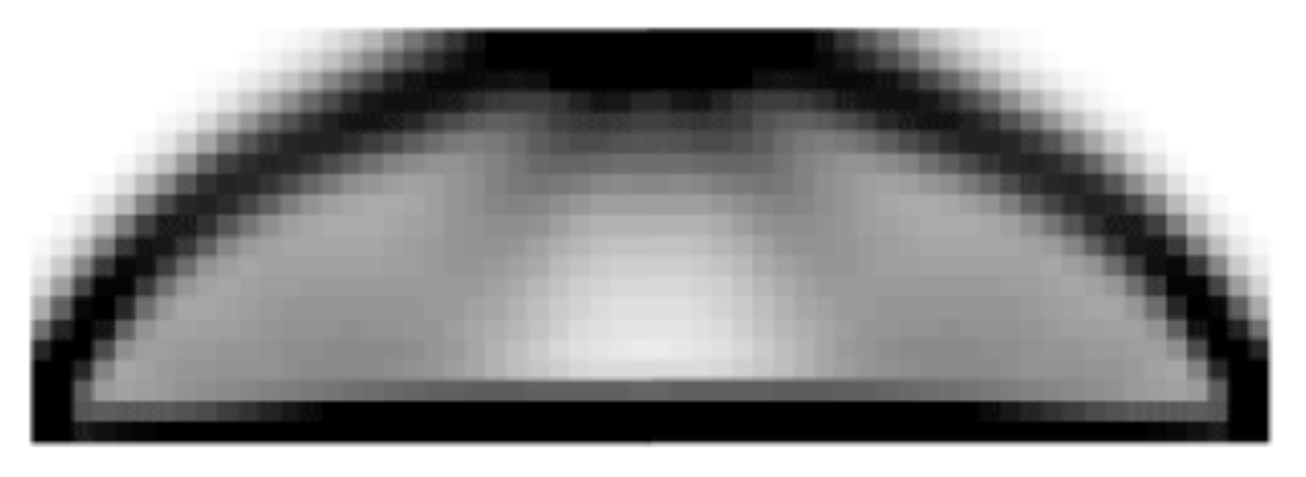
\includegraphics[scale=0.25]{Dissertation/images/grey_fig} 
	
\includegraphics[scale=0.2]{Dissertation/images/black_fig} 
	\caption{Пример серой и черно-белой конструкций}\label{fig:grey_fig}
\end{figure}

%В SIMP лучше использовать $p > 1$, чтобы промежуточные плотности были неблагоприятны в том смысле, что полученная жесткость мала по сравнению с объемом материала. 
%Для задач, в которых действует ограничение на объем, оптимизация действительно приводит к искренним конструкциям <<0-1>>, если выбрать p достаточно большим~($p > 3$). 

%В дальнейшем метод был расширен для задач с несколькими материалами. О.~Зигмунд и С.~Торквато усовершенствовали схему интерполяции материала по закону мощности~\cite{Sigmund1997}. Д.~Стегман и Е.~Лунд адаптировали SIMP для дискретной оптимизации анизотропных материалов~(DMO)~\cite{Stegmann2005, Lund2006}. Эти усовершенствования сделали метод более универсальным и подходящим для оптимизации конструкций из нескольких материалов.

%Метод SIMP имеет ряд недостатков связанных с непрерывностью значения плотности. Чтобы избежать этих проблем, необходимо выбирать подходящий коэффициент пенализации.

%Метод SIMP отличается простотой реализации и широким применением в различных областях проектирования, таких как механика, аэродинамика и энергетика. 
%Тем не менее, для минимизации нежелательных эффектов, таких как промежуточные плотности, ключевую роль играет выбор коэффициента пенализации и параметров сетки.

%Метод SIMP стал базовым инструментом топологической оптимизации благодаря своей интуитивной понятности и гибкости. Он продолжает совершенствоваться, оставаясь актуальным инструментом для решения сложных инженерных задач.

\subsection{Методы эволюционной структурной оптимизации (ESO)}

Метод эволюционной структурной оптимизации~(Evolutionary Structural Optimization) был предложен Й.\,М.~Кси и Г.\,Ф.~Стивеном в начале~1990-х годов~\cite{Xie1993,Xie1997} и представляет собой один из наиболее активно развивающихся подходов в топологической оптимизации. 
Этот метод предполагает постепенное удаление малонагруженных элементов конструкции, что позволяет оставлять только области, подверженные максимальным напряжениям. 
В отличие от метода SIMP, где используются непрерывные значения плотности, метод ESO основан на бинарных значениях плотности~$x\in\{0,1\}$.

Основная идея заключается в том, чтобы привести конструкцию к состоянию, в котором напряжение во всех оставшихся элементах будет близко к допустимому пределу.           
%Изначально метод использовал уровень напряжения в качестве индикатора для удаления неэффективного материала, ожидая, что в результате эволюции структура достигнет своей оптимальной топологии. 
%Но в целом подход позволяет применять и другие показатели чувствительности для управления процессом эволюции. На каждой итерации удаляются элементы с минимальным вкладом в общую производительность конструкции, причем объем удаляемого материала регулируется параметром отношения удаления.

%Метод Evolutionary Structural Optimization (ESO) заключается в удалении лишнего материала из конструкции. Индикатором неэффективного использования материала является низкий уровень напряжений (или деформаций) в этой части. Предпочтительным является такое распределение материала, при котором уровень напряжений в конструкции близок к предельному, но безопасному значению, и распределен равномерно. Отсюда следует принцип удаления материала, согласно которому недостаточно нагруженный материал может быть удален. Для того, чтобы избежать перестроения конечноэлементной сетки, удаление материала производится путем присвоения удаляемому элементу эффективных свойств псевдоматериала, имитирующего пустоту. 

Развитие метода ESO привело к появлению его модификаций. 
Обратный метод AESO~(Additive Evolutionary Structural Optimization)~\cite{Querin2000} основан на добавлении материала в наиболее нагруженные области конструкции. 
ESO и AESO являются однонаправленными методами, что ограничивает их применение в сложных задачах, где важно учитывать возможность возвращения ранее удаленного материала. Для преодоления этих ограничений был разработан двунаправленный метод BESO~(Bi-directional Evolutionary Structural Optimization){\cite{Querin1998, Yang1999}}. Метод BESO сочетает принципы ESO и AESO, позволяя как удалять материал, так и возвращать его обратно. В этом методе удаленные элементы с наибольшими значениями чувствительности возвращаются в систему, а заполненные элементы с минимальными значениями чувствительности~--- удаляются. 

Число удаляемых и добавляемых элементов на каждой итерации определено двумя независимыми друг от друга параметрами: коэффициентом удаления $c_{rr}$ и коэффициентом включения $c_{rr}$. 

При дискретизации непрерывной структуры на конечные элементы функция чувствительности может терпеть разрыв на границах элементов, что ведет к образованию топологии в виде <<шахматного поля>>~(рисунок~\cref{fig:chess_topology}).

\begin{figure}[ht]
	\centering 
	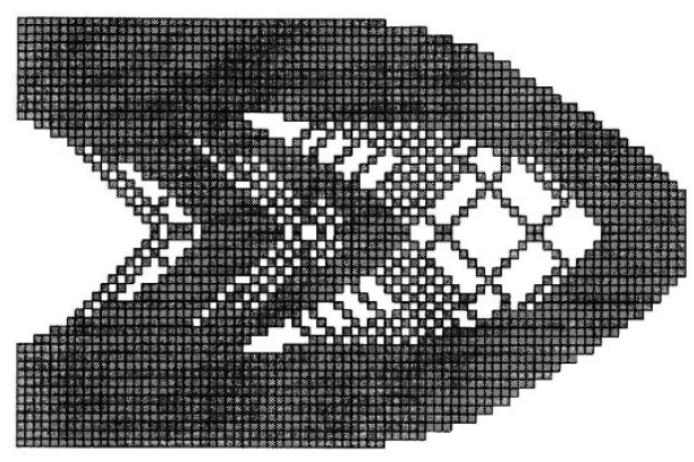
\includegraphics[scale=0.5]{Dissertation/images/chess.png} 
	\caption{Пример топологии <<шахматного поля>>}\label{fig:chess_topology}
\end{figure}

Для того чтобы избежать подобного результата используется сглаженная чувствительность элементов с фильтрацией, причем характерный размер фильтра $r_{min}$ не меняется с изменением сеточного разбиения. Величина $r_{min}$ создает круговую подобласть $\Omega_i$, центр которой совпадает с центром $i$-го элемента. Подобласть   накрывает несколько соседних элементов. Элементы, центры которых расположены внутри   создают вклад в сглаженную чувствительность $i$-го элемента согласно формуле

%\begin{equation}\label{eq:alpha}
%\begin{aligned}
%\alpha_i = \frac{\sum_{j=1}^K w(r_{ij}) \alpha_j^n}{K},
%\end{aligned}
%\end{equation}
\begin{equation}\label{eq:alpha}
	\begin{aligned}
		\alpha_i = \left(\sum_{j=1}^K w(r_{ij})) \alpha_j^n \right)/K,
	\end{aligned}
\end{equation}
где $K$~--- общее число узлов, содержащихся в подобласти $\Omega_i$, и $w(r_{ij})$~--- линейные веса, определяемые как

\begin{equation}\label{eq:w}
	\begin{aligned}
		w(r_{ij}) = \frac{r_{min}-r_{ij}}{K},
	\end{aligned}
\end{equation}

Таким образом, сглаживая значения чувствительности по всей области проектирования, схема фильтрации автоматически присваивает ненулевые значения чувствительности удаленным элементам. Для исключения значительных осцилляций минимизируемого функционала и резких изменений соответствующей топологии в итерационном процессе используется усреднение индексов чувствительности между текущим и предыдущим шагами оптимизации~\cite{Shevtsov2014}.

\begin{equation}\label{eq:w}
	\begin{aligned}
\alpha_i = \frac{\alpha_i^k - \alpha_i^{k+1}}{2},
	\end{aligned}
\end{equation}
где $k$~--- номер текущей итерации. На следующей итерации полагают $\alpha_i=\alpha_i^{k+1}$ и~т.~д. 

%Они внедрили схему фильтрации чувствительности, стабилизирующую процесс оптимизации с учетом истории изменений. Это позволило значительно расширить области применения метода, включая задачи оптимизации сложных конструкций с несколькими материалами.

Современные эволюционные методы подразделяются на две группы: подходы hard-kill и soft-kill. В hard-kill подходе материал удаляется полностью, что может вызвать проблемы со сходимостью метода. В soft-kill~\cite{Ghabraie2015}~--- удаление материала осуществляется плавно, через снижение модуля упругости элемента, что делает процесс оптимизации более стабильным и позволяет достичь высококачественных решений.

\subsubsection{soft-kill}

%Эволюционные методы продолжают активно развиваться, внедряются новые алгоритмы и расширяется их применение в различных задачах. Такие подходы остаются востребованными благодаря их гибкости, особенно при решении задач, требующих учета сложных физических ограничений и многоматериальных систем.

\subsection{Методы на основе генетических алгоритмов}


\subsection{Методы на основе нейронных сетей}

В последние несколько лет наблюдается рост числа публикаций с применением AI-фреймворков при решении задач топологической оптимизации.

Литературу по применению машинного обучения в задачах топологической оптимизации можно разделить на пять основных групп~\cite{Woldseth2022}. Эти категории определяются как прямое проектирование, акселерация, постобработка, редукция и разнообразие дизайна. 





Прямое проектирование относится к стратегии создания обучающих моделей для непосредственного прогнозирования оптимальной структуры при задании некоторых описательных характеристик проблемы, и как таковая цель состоит в том, чтобы достичь оптимальных структур без итераций.

Этот подход в настоящее время является одним из самых популярных применений ИИ в топологической оптимизации, и его цель состоит в том, чтобы напрямую достичь оптимизированной структуры для заданного определения проблемы, полностью устранив необходимость в дорогостоящих итеративных процедурах. Обычно это достигается за счет реализации архитектур нейронных сетей, популярных в сегментации изображений, таких как CNN или GAN. Представление структурного проекта обычно определяется плотностью элементов в регулярной сетке КЭ, аналогично подходу SIMP. (Zheng et al. 2021b; Hoang et al. 2022).

Входные данные модели состоят из граничных условий, приложенных сил и объемной доли, заданных в пространственном представлении последовательностью входных матриц с размерами, равными размерам рассматриваемой КЭ-сетки. Обученная сеть затем используется для сопоставления этих входных данных с некоторым окончательным структурным проектом, либо путем регрессии в виде непрерывных значений плотности элементов по шкале серого, либо путем классификации в виде двоичных черно-белых значений, указывающих на наличие материала в элементе или его отсутствие. 

Большинство моделей прямого проектирования обучаются в контролируемом (CNN) или полуконтролируемом (GAN) режиме, где большое количество оптимизированных структур используется в качестве целевых образцов для обучения. Это означает, что для каждого рассматриваемого в процессе обучения проблемного случая должен быть выполнен как минимум один полный прогон обычных ТО. Большинство моделей прямого проектирования сосредоточены на проблемах с фиксированными или очень похожими условиями опоры, изменяя только объемную долю и приложенные нагрузки, где количество и возможные размещения нагрузок обычно также имеют ограничения.

Если сетевая архитектура разработана специально для определенных размеров сетки, то размер сети увеличивается с увеличением количества элементов в сетке, что приводит к большему количеству параметров, которые необходимо определить во время обучения, и большему потреблению памяти для хранения модели. По-видимому, такая воспринимаемая сетчатая зависимость моделей прямого проектирования является ограничивающим фактором для исследований в рамках этого класса подходов. Кроме того, затраты на создание обучающих выборок с высоким разрешением и повышенная структурная сложность, связанная с КЭ-сетками с более высоким разрешением, вероятно, являются определяющими факторами, объясняющими, почему в большей части современной литературы рассматриваются только сетки с низким разрешением, обычно содержащие не менее 4 000 элементов и не более 26 000 элементов (Lei et al. 2019; Li et al. 2019; Zheng et al. 2021c).








Акселерация относится к моделям обучения, используемым в качестве дополнения к традиционным методам итерационного решения с целью снижения вычислительных затрат. Обычно это достигается путем замены конечноэлементного анализа некоторой приближенной моделью в подмножестве итераций или путем построения прямого отображения между промежуточными структурами, эффективно пропуская некоторое подмножество итераций.

Применение методов искусственного интеллекта для ускорения ТО привлекает все большее внимание, поскольку подходы направлены как на ограничение количества итераций, так и на сложные вычисления, необходимые в рамках обычной процедуры итерационной оптимизации. Стратегии в этой категории предлагают более разнообразный профиль, чем для ранее описанных моделей прямого проектирования, но есть некоторые ключевые сходства в мотивационных идеях, лежащих в основе представленных работ.

Анализ чувствительности Считается, что метод ИИ применяется к анализу чувствительности, когда цель состоит в том, чтобы заменить или уменьшить потребность в точных оценках чувствительности. Некоторые из работ (Aulig and Olhofer 2013; Olhofer et al. 2014; Aulig and Olhofer 2015), содержащиеся в этом разделе, применимы только в том смысле, что они действительно способствуют ускорению, в тех случаях, когда чувствительность трудно получить с помощью обычного анализа методом конечных элементов и совместного анализа. Утверждение о существовании таких проблем ТО часто можно услышать, но редко приводит в пример. Другие работы (Chi et al. 2021; Цянь и Е 2021; Keshavarzzadeh et al. 2021b) пытаются снизить вычислительную нагрузку или полностью исключить анализ конечных элементов, необходимый в процессе TO.

Общим для этих подходов является то, что они нацелены на обучение модели аппроксимации сложных вычислений по некоторому функциональному соотношению. С этой целью некоторая нейронная сеть с прямой связью конструируется и обучается в виде регрессионной модели с использованием контролируемого обучения. Как правило, входные данные сети состоят по крайней мере из текущей плотности элементов. В некоторых случаях также учитываются условия нагружения, а для процедур, где МКЭ все еще присутствует в той или иной форме, также подаются энергии смещения или деформации.

Один проход через сеть может применяться к одному отдельному элементу, участку элементов внутри структуры или ко всем элементам структуры одновременно. Подходы, учитывающие только подмножества элементов за раз, могут обеспечить повышенную способность к обобщению, поскольку сетчатые и проблемные зависимости потенциально уменьшаются, но, с другой стороны, важная глобальная информация может быть упущена из виду. Кроме того, КЭ-анализ отдельной структуры и истории ее плотности может предоставить больший набор обучающих выборок с различными характеристиками. Таким образом, генерация данных в большинстве случаев значительно дешевле, чем для моделей прямого проектирования, и существует потенциал для естественного захвата большего разнообразия входных данных. Рассматривая такие подструктуры, можно ожидать, что сходство между данными обучения и испытаний увеличится, даже при совершенно разных граничных условиях и загружениях.

Lee et al. (2020) предложили структуру решения, основанную на традиционном методе критериев оптимальности (OC), в котором две отдельные модели CNN обучаются для прогнозирования соответствия и объемной доли соответственно. Для соответствия это означает, что отпадает необходимость в оценке структурной целостности с помощью МКЭ, что заменяет расчеты на менее сложную функциональную аппроксимацию. Обычное вычисление объемной дроби имеет линейную сложность, которая теперь заменена некоторой нелинейной функцией, представленной соответствующей СНС. Общая идея заключается в том, что эти нейронные сети снизят вычислительную нагрузку на каждой итерации в процессе оптимизации, что приведет к значительному ускорению. Большинство представленных экспериментальных результатов сосредоточены на способности сети прогнозировать объемную долю и податливость для данной структуры, и, таким образом, интеграция модели в процесс TO, где требуется чувствительность элементов, не детализирована. В статье рассматриваются MBB-балка и консольная балка с фиксированной дискретизацией сетки и различными объемными дробями, как для обучения, так и для тестирования. Поэтому полная оценка эффективности метода затруднена из-за большого сходства между учебными и тестовыми случаями. Papadrakakis et al. (1998) и Sasaki and Igarashi (2019) аналогичным образом представили ИНС, обученные прогнозировать объективные и ограничивающие значения структуры, направленные на замену оценок пригодности в каждой итерации GA-структуры. Qiu et al. (2021) обучили сети итеративному удалению материала из полностью твердой области, аналогично эволюционной структурной оптимизации, но без использования МКЭ в реальной процедуре оптимизации.

Aulig and Olhofer (2013); Olhofer et al. (2014) и Aulig and Olhofer (2015) сосредоточились на разработке ML-моделей регрессионного типа для прогнозирования чувствительности, когда сопряженный подход недостижим (не продемонстрирован в их работе), так что конечная дифференциация является единственной альтернативой. В качестве примеров используются задачи минимизации соответствия стандартам, для которых известны формулы точной чувствительности. Входные данные модели связаны с плотностями и перемещениями элементов (вычисленными по методу конечных конечных моделей). При минимизации соответствия точный градиент элемента относительно цели является функцией тех же самых особенностей. Это означает, что можно ожидать хороших показателей с точки зрения точности чувствительности для данной конкретной постановки задачи, но нельзя делать никаких выводов о переносимости на другие формулировки. Также представлена структура для дальнейшего ограничения вычислительных затрат на конечную дифференциальную альтернативу. Здесь вычислительная нагрузка МКЭ снижается за счет адаптивной выборки элементов, необходимых для точной оценки, что снижает степени свободы в МКЭ. Однако эта стратегия не имеет отношения к ML или NS и, таким образом, выходит за рамки данного обзора.

Если желаемым эффектом модели является снижение вычислительной нагрузки МКЭ, но не обязательно полное исключение этого метода анализа из процедуры оптимизации, другим вариантом обучения модели является облегчение онлайн-обучения. Онлайн-обучение означает, что модель обучается не на предварительно собранных данных, а в процессе применения для адаптации к конкретной проблеме. Для рассматриваемой цели это означает, что модель обучается во время прогона оптимизации, где МКЭ затем завершается только в подмножестве итераций, а полученные решения используются в процедуре последовательного обучения передачи с возрастающим числом выборок данных. Chi et al. (2021), а также Zhang et al. (2021a) представили такой подход, при котором после каждого набора новых обучающих данных проводится процедура, основанная на передаче обучения, чтобы итеративно сделать модель более точной. Авторы предлагают выполнять оптимизацию в виде двухмасштабного подхода, при котором грубая сеточная версия структуры подвергается воздействию МКЭ на каждой итерации, в то время как обученная модель применяется для отображения этих результатов на более мелкую сетку, где МКЭ применяется только на подмножестве итераций. Эти подходы, как таковые, не только связаны с анализом чувствительности, но и используют многоуровневый подход TO для получения вычислительных сокращений, связанных с анализом чувствительности. Представленные результаты показывают, что перспективность и точность прогнозов чувствительности тонкой сетки, по-видимому, улучшаются с помощью этого онлайн-подхода. Подход и результирующее ускорение аналогичны методам с несколькими разрешениями (Groen et al. 2017; Nguyen et al. 2012).

Основные задачи для ИНС, направленные на снижение вычислительных затрат, затрачиваемых на МКЭ при оптимизации, имеют двоякое значение. Во-первых, некоторые подходы основываются на ошибочных предпосылках, когда традиционные альтернативы считаются менее эффективными, чем они есть на самом деле, что делает эти подходы излишними. Во-вторых, модели, разработанные для очень специфических проблемных случаев, становятся слишком ограниченными, чтобы их можно было использовать в качестве общей основы для TO. Что касается подходов к онлайн-обучению с несколькими разрешениями, они могут быть подвержены влиянию грубых сетчатых ограничений мелких элементов при проецировании на более высокое разрешение. Это явление характерно для рассмотренных двухмасштабных методов и будет рассмотрено более подробно при рассмотрении категории масштабирования в разделе 2.2.3.

Сходимость Если модель обучена сопоставлению между промежуточными структурами решения с целью уменьшения общего числа итераций в процедуре оптимизации, то говорят, что она относится к ускорению сходимости. Типичный выбор методов основан либо на модели, похожей на прямой дизайн (Ye et al. 2021; Joo et al. 2021) или прогнозирование, основанное на временных рядах (Kallioras et al. 2020). Модели прямого проектирования отображают входное изображение в оттенках серого промежуточной конструкции с почти сходящейся структурой. В качестве альтернативы, методы, основанные на временных рядах, рассматривают траектории плотностей отдельных элементов и стремятся напрямую отобразить каждый элемент от данной итерации до состояния, близкого к сходящемуся.

Первый подход наследует большинство проблем, связанных с моделями прямого проектирования. Если необходимо отобразить полное изображение сразу, построенная модель, скорее всего, будет зависеть от сетки. Обеспечение разнообразия и точности для различных характеристик задачи является сложной задачей и сопряжено с большими вычислительными затратами, связанными с генерацией выборки данных. Тем не менее, он выигрывает от того, что в качестве сетевых входных данных доступно больше описательных данных. Из выполненных итераций оптимизации, используемых для получения промежуточной структуры, известны как поле перемещения, так и история плотности элементов, которые могут быть использованы в качестве входных данных для модели.

Сосновик и Оселедец (2017) обучили CNN переводить изображение структуры в оттенках серого, полученное после k итераций SIMP, в окончательный черно-белый дизайн. Обучающий набор данных был сгенерирован путем выполнения 100 итераций SIMP по псевдослучайным формулировкам задач на сетке 40x40. В качестве входов в сеть используются плотности элементов на итерации 
и последнее изменение плотностей по сравнению с итерациями 
Для итерации K поставляются в виде двух изображений в оттенках серого. Были протестированы различные стратегии выборки k в каждой обучающей выборке, и выходной целью рассматривалось черно-белое изображение, полученное путем порогового значения оптимизированной структуры при 
. Показано, что обученная модель превосходит стандартные пороговые значения для обучающего набора данных, но при тестировании на новых задачах, проблемах теплопроводности, производительность становится аналогичной. Эксплуатационные характеристики измеряются двоичным сходством между структурами, и никаких показателей соответствия или объемной доли полученных структур не сообщается. Структурные результаты также иллюстрируются для задач, аналогичных обучающим выборкам данных на более тонких сетках (до 72x108 элементов), но эффект, по-видимому, заключается в простом сглаживании границ по сравнению с более грубыми структурами. Joo et al. (2021) предложили аналогичный подход, но вместо того, чтобы сразу отобразить всю структуру, их модель разделила структурное изображение на перекрывающиеся подмодули, которые затем по отдельности сопоставляются с оптимизированной подструктурой, а полная структура впоследствии получается путем интеграции по этим подмодулям.

Одно из преимуществ рассмотрения структурного образа как участков или целого, а не по элементам, заключается в том, что некоторая информация о взаимодействии между элементами может быть сохранена и изучена CNN. Однако в подходе, основанном на временных рядах, существует предположение о независимых траекториях плотности каждого элемента, что может быть проблематичным именно из-за того, что элементы должны иметь соответствующее взаимодействие для формирования жизнеспособной структуры. Некоторые из этих взаимодействий могут быть наблюдаемы для сети, учитывая сходство в их итеративных историях плотности до применения отображения. Преимущество этого подхода заключается в том, что обобщающая способность предложенного метода, вероятно, возрастет, поскольку в обучающих выборках отражается меньшая зависимость от сетки и проблемы. Успех этого метода, однако, зависит от схожести ожидаемых итерационных траекторий даже при разных постановках задач. Движущийся элемент конструкции приведет к траекториям колоколообразного типа, что означает, что направление траектории плотности и траектории соответствующих элементов изменится несколько раз в течение всей истории итераций. Таким образом, предполагается, что траектория плотности элемента в течение первых нескольких итераций достаточна для того, чтобы различить элементы, для которых это происходит, независимо от того, какая структурная проблема рассматривается.

Kallioras et al. (2020) предложили подход на основе временных рядов, в котором итеративные истории плотности элементов за первые 36 итераций SIMP использовались в качестве входных данных для нейронной сети, которая индивидуально сопоставляет плотности элементов с близкими к сходящимся значениям для формирования структуры, от которой SIMP продолжается до сходимости. Используемая модель представляет собой сеть глубокого убеждения (DBN), которая представляет собой тип ИНС, в которой обнаружение признаков для достижения уменьшения размерности проводится в каждом слое. Таким образом, входной вектор истории итерационной плотности элемента постепенно уменьшается до конечного значения плотности по всей сети. Сеть была обучена на выборках данных, состоящих из итерационной истории, полученной из решения версий консольных и просто опорных балок с различными масштабами длины и дискретизациями. Количество конечных элементов в этих обучающих выборках варьировалось от 1 000 до 100 000, где для каждого разрешения были решены четыре набора граничных условий для двух разных масштабов длины. При тестировании модели на задачах, отличных от обучающих случаев, достигается ускорение вычислений. Об ускорении сообщается с точки зрения количества итераций SIMP, необходимых для достижения сходимости, по сравнению с традиционным подходом. Полученные решения имеют значения соответствия, примерно соответствующие значениям полученных SIMP бенчмарков. Следует отметить, что сравнения с традиционным SIMP-подходом проводятся в серой шкале, которая, как показано на рис. 4 может быть значительно недооценена фактическая жесткость конструкции, и поэтому сравнительные результаты могут быть нерепрезентативными.

Общим для представленных приложений сходимости является то, что они предполагают, что часть итерационной истории плотности на ранних этапах процедуры оптимизации достаточна для определения характера конечного результата. Это может быть проблематичным предположением для проблемных случаев, когда элементы конструкции перемещаются во время оптимизации, вызывая большие изменения как в плотности отдельных элементов, так и в поле плотности в целом. Подход с временными рядами, основанный на индивидуальной истории плотности пикселей, особенно маловероятен, но все еще может существовать потенциал для подходов, учитывающих глобальное изменение структуры (Muñoz et al. 2022). Разумно предположить, что с учетом предыдущей истории итераций можно предсказать изменение плотности после подмножества последовательных итераций, но, исключив значительную часть итерационного поиска, вероятно, столкнется с теми же проблемами, что и при непосредственном проектировании.






Постобработка определяется как модификация структур, полученных с помощью обычной топологиесой оптимизации или гомогенизации, обычно направленной на обеспечение технологичности путем изменения формы, определения конфигураций микроструктуры, сглаживания границ или в качестве замены подходов к дегомогенизации.

Методы искусственного интеллекта рассматриваются как процедуры постобработки, когда для генерации входных данных модели используется оптимизированная структура. Таким образом, данная категория приложений относится к методам интерполяции данной структуры для более точного разрешения сетки или оптимизации формы и извлечения признаков в целях технологичности.

Оптимизация формы Когда целью сформулированной модели является изменение особенностей полученной структуры для обеспечения удовлетворения практических и экономически эффективных требований технологичности, считается, что метод выполняет постобработку путем оптимизации формы. Эстетика дизайна также может мотивировать такие приложения, когда, например, Vulimiri et al. (2021) рассматривали TO для минимального соответствия, придерживаясь при этом некоторого эталонного дизайна для структурных узоров, таких как круги или паутина.

Две работы, представленные в этой категории, Lin and Lin (2005) и Yildiz et al. (2003), предложили версии ИНС, предназначенные для классификации отверстий в структуре, оптимизированной для TO. Лин и Лин (2005) предложили двухступенчатую процедуру, в которой первая ИНС обучается распознавать основную геометрическую форму отверстия при получении входных данных в виде инвариантных моментов, описывающих геометрические характеристики отверстия в оптимизированной структуре. Второй этап состоит из нескольких ИНС, по одной для каждой группы базовой геометрии, определенной для первой ИНС, и каждая из них обучается подгонке под подробный шаблон формы для отверстия в рамках своей группы базовой геометрии. Используемый формат входных данных представляет собой набор расстояний и соотношений площадей изображения отверстия, представленного независимым от размеров способом, и сеть использует эту информацию для отображения отверстия на один из двенадцати предопределенных шаблонов геометрических форм в рассматриваемой категории форм. Yildiz et al. (2003) обучили одну ИНС, которая использует в качестве входных данных изображение структуры, оптимизированной для TO, в оттенках серого и вычисляет доверительные меры для каждой дыры в структуре, основываясь на предполагаемом сходстве с четырьмя основными шаблонами признаков. Выявленные формы отверстий затем используются для формулирования модели детали на основе элементов, которая подвергается оптимизации формы для получения желаемой окончательной структурной компоновки. Основные проблемы, связанные с представленными работами, связаны с тем, что обе они опираются на вручную определенные наборы возможных форм. Кроме того, поскольку размеры этих наборов ограничены, неясно, будет ли получено что-либо от применения моделей на основе искусственного интеллекта для выполнения задач идентификации. Yildiz et al. (2003) также обнаружили, тестируя различные архитектуры ИНС, что наилучшие результаты достигаются, когда ИНС содержит только один скрытый слой. В связи с этим возникает вопрос о том, могут ли альтернативные и более простые детерминистические методы достичь аналогичных результатов.

Hertlein et al. (2021) предложили модель GAN прямого проектирования с интегрированными производственными ограничениями для аддитивного производства и объединили ее с процедурой постобработки с использованием обычного TO. Входные данные для модели состоят из каналов, непосредственно относящихся к рассматриваемой сетке 64x64, указывающих на опоры и нагрузки, а также ориентацию рабочей плиты с учетом технологичности. Входное кодирование построено таким образом, что существование материала поощряется в элементах, где ожидается, что оптимизированная структура будет иметь материал, определяемый здесь местоположением нагрузок и строительной пластины. Выходными данными GAN является изображение в оттенках серого, представляющее оптимизированную топологию. Обучающие данные получены с помощью обычного TO (Andreassen et al. 2011) со встроенным фильтром вылета, как представлено Langelaar (2017). Также предлагается, чтобы результирующая структура подвергалась постобработке путем выполнения некоторого количества итераций этой традиционной альтернативы, чтобы еще больше устранить выступающие элементы и исправить любые неточности, связанные с соответствием.

В целом, данный вид применения AI-технологий недостаточно изучен в литературе. Это может быть связано с введением фильтров и ограничением технологичности в процессе формулировки и решения задачи TO, что снижает потребность в постобработке, или с тем, что существуют альтернативные традиционные методы постобработки с удовлетворительными характеристиками. Было бы очень полезно, если бы машинное обучение можно было использовать для извлечения CAD-геометрии из оптимизированных конструкций, поскольку многие методы производства требуют формата структурного представления, который не может быть напрямую получен из конструкций, основанных на плотности. Жизнеспособность получения такой модели, однако, не гарантируется. Существует обширная литература по методам обратного инжиниринга (Buonamici et al. 2018). Эти методы реконструируют модели САПР на основе полученных 3D-данных в виде треугольных сеток или облаков точек. Некоторые методы позволяют создавать модели конструктивной твердотельной геометрии (CSG) (Du et al. 2018). Эти методы часто основаны на обнаружении примитивных форм на входе (Li et al. 2011), в то время как Эк и Хоппе (1996) генерировали участки B-сплайна из входных данных. Такие методы могут быть использованы для постобработки TO-оптимизированных структур.

Масштабирование В работах, относящихся к категории постобработки апскейлинга, обычно рассматривается грубая сетчатая структура, оптимизированная с помощью традиционных методов, и применяется некий тип нейронной сети для перевода этой структуры в более мелкую сетку. Существуют различные подходы к форматированию входных данных для рассматриваемой модели: Wang et al. (2021a) и Yu et al. (2019) оценивали весь структурный образ плотности элементов в качестве входных данных, в то время как Napier et al. (2020) и Xue et al. (2021) разделили структуру на участки плотности элементов, которые обрабатываются индивидуально, но могут иметь некоторое перекрытие с точки зрения принадлежности элементов к каждому участку. Последний вариант, вероятно, будет наиболее выгодным с точки зрения способности к обобщению, тем более что модели могут быть более или менее независимыми от сетки. Кроме того, подход, основанный на патчах, может позволить использовать меньше оптимизированных структур с высоким разрешением для обучающих данных, и, таким образом, может быть достигнута общая значительная экономия вычислительных затрат. Однако одна из проблем заключается в том, что прикладная модель не имеет никакого понятия структуры в целом, так что получается только тонкая настройка границ и не уточнение топологии.

Каллиорас и Лагарос (2021) предложили метод (DL-шкала), который несколько отличается от этого подхода, поскольку они применяют детерминированное масштабирование, итеративно сопряженное со структурой ускорения сходимости DBN, предложенной в Kallioras et al. (2020). Таким образом, в данной работе не используется методология искусственного интеллекта для фактического масштабирования, но она упоминается здесь, поскольку представленные результаты по-прежнему отражают некоторые общие проблемы в этой категории. Несмотря на то, что они действительно наблюдают значительное ускорение для все более тонких сеток, становится очевидным, что решения, полученные с помощью модифицированного подхода, имеют меньшую способность улавливать более мелкие элементы по сравнению с соответствующими структурами, оптимизированными для SIMP. Кроме того, в некоторых из описанных случаев уровень шкалы серого кажется более высоким для структур, полученных в масштабе DL, и поскольку минимальные соответствия, сравниваемые в каждом тестовом случае, рассчитываются для изображений в оттенках серого, неясно, являются ли в действительности репрезентативными общие более высокие объективные значения, полученные с использованием шкалы DL. Отсутствие более тонких структурных компонентов при применении масштабирования является обычным явлением в литературе, и такие работы, как Wang et al. (2021a), иллюстрируют, как попытка захватить мелкие детали может привести к структурам с большой степенью размытых серых областей или даже структурных разъединения. По сути, детали в мелком масштабе ограничены грубым разрешением масштаба, которое эффективно работает как грубое ограничение длины и масштаба.

Elingaard et al. (2022) предложили СНС для сопоставления набора параметров ламинирования на грубой сетке с мелкомасштабным дизайном, способствующим очень мелким элементам. Сеть как таковая используется в качестве вычислительно эффективной замены для дегомогенизации (Pantz and Trabelsi 2008; Groen and Sigmund 2018) для преодоления существующего узкого места в экстракции мелкомасштабных отложений приводит к оптимизации топологии на основе гомогенизации. В качестве входных данных для сети используются ориентации из решения TO на основе гомогенизации. Затем сеть используется для повышения дискретизации этой информации до промежуточного поля плотности, которое обрабатывается с использованием последовательности графических шагов, выполняемых в линейном времени, для получения окончательного одномасштабного проекта с высоким разрешением. Обучение без учителя используется для того, чтобы избежать необходимости генерировать дорогостоящие мишени, а дешевая генерация входных данных для обучения обеспечивается путем выборки из суррогатного поля низкочастотных синусов. Обучение как таковое выполняется независимо от физических свойств лежащей в основе задачи структурной оптимизации, что делает метод независимым от сетки и задачи. С помощью численных экспериментов было обнаружено, что этот подход обеспечивает ускорение в 5-10 раз по сравнению с современными подходами к дегомогенизации.

Общим для представленных двухмасштабных подходов, направленных на преобразование структурной информации из грубой сетки в тонкую с использованием одних и тех же мер, в основном плотностей или чувствительности, является то, что грубая масштабная сетка накладывает ограничения по длине на тонкую сетку. Это означает, что использование ИНС для выполнения этого сопоставления позволяет получить мало информации по сравнению с традиционными методами интерполяции. Эта проблема не возникает, если ИНС применяется для дегомогенизации, поскольку в данном случае она служит инструментом для замены вычислительного процесса, который является частью ранее существовавшей схемы масштабирования, где детали конструируются из грубой масштабной информации на основе заранее определенных правил.







Редукция выполняется с целью уменьшения размера проектного пространства путем построения модели, которая описывает топологию более компактным образом. Эта повторная параметризация позволяет выполнять итеративную оптимизацию с меньшим количеством проектных переменных, что значительно ускоряет процедуру решения. Такие подходы напоминают стандартные методы уменьшения порядка моделей, но с той разницей, что природа подходов ИИ отличается, поскольку они не запрограммированы явно.%%%

Типичный подход к достижению редукции или перепараметризации проблемы с помощью методов искусственного интеллекта заключается в построении одной или нескольких взаимосвязанных нейронных сетей с целью представления структуры с использованием меньшего количества проектных переменных и, таким образом, снижения вычислительной нагрузки на процедуру оптимизации. Это может быть сделано путем обучения VAE для извлечения признаков и использования уменьшенной размерности полученного латентного пространства для проведения оптимизации на этом латентном векторе. В качестве альтернативы, сеть может быть построена в качестве прямого суррогата процесса оптимизации таким образом, чтобы обучение сети было эквивалентно решению данной задачи оптимизации, используя при этом, что параметры и смещения сети достаточны в качестве проектных переменных.

Guo et al. (2018) рассмотрели многокритериальную задачу теплопроводности, для которой VAE обучается контролируемым образом, с целью минимизации ошибки реконструкции сети энкодер-декодер. Затем модель проверяется путем интеграции в различные традиционные среды оптимизации, включая методы на основе градиента, генетические алгоритмы и гибридные версии этих двух методов. Кодируя промежуточную структуру, можно выполнять обновления дизайна в уменьшенном скрытом пространстве. Затем новый латентный вектор может быть преобразован в интерпретируемую структуру декодером, который затем подвергается физическому анализу. Таким образом, МКЭ по-прежнему необходима для всего пространства проектирования, используя ту же дискретизацию сетки, что означает, что вычислительные затраты на вычисление объектива и чувствительности остаются такими же, как и для традиционных методов. Тем не менее, может быть потенциальный выигрыш в производительности за счет сокращения количества необходимых итераций, поскольку количество МКЭ, которые, как сообщается, достигают сходимости, варьируется в зависимости от различных протестированных фреймворков решений. Тем не менее, сообщается о небольшом количестве тестовых случаев и проводится мало сравнений с современными процедурами.

Чандрасекар и Суреш (2021c) использовали ИНС для повторной параметризации функции плотности и, таким образом, в принципе сделали представление плотности независимым от сетки КЭ. При интеграции нового структурного дескриптора в традиционную структуру решения веса и смещения ИНС становятся проектными переменными, которые оптимизируются с помощью неконтролируемого обучения с функцией потерь, соответствующей взвешенной сумме структурной податливости и нарушения ограничений по объему. Это эквивалентно традиционной оптимизации нового проектного представления, что означает, что сеть не подвергается какому-либо реальному обучению. Таким образом, это пример использования ИНС без обучающего аспекта.

Позже Чандрасекар и Суреш (2021b) показали, как эта структура может быть распространена на задачу TO из нескольких материалов, где распределение двух или более материалов в структуре получается одновременно с оптимизированной топологией, а Чандрасекар и Суреш (2021a) добавили расширение ряда Фурье в ИНС, чтобы навязать управление масштабом длины. В любом случае МКЭ оценивается на одной и той же сетке КЭ, которая в каждой итерации строится путем выборки плотностей для необходимых пространственных координат с использованием ИНС. Таким образом, обычный физический анализ дискретизированной сетки по-прежнему необходим для вычисления чувствительности объекта (в данном случае также функции потерь) по отношению к плотности элементов, после чего чувствительность по отношению к параметрам сети может быть определена с помощью классического обратного распространения. Многообещающей особенностью этого приложения является то, что благодаря аналитическому представлению плотности-поля можно получить более четкие структурные границы. В настоящее время, однако, структуры проецируются на фиксированную сетку КЭ для анализа, что означает, что граница фактически размыта. Кроме того, происходит потеря мелких деталей в структурах, полученных с помощью новой процедуры решения, и детализация, по-видимому, не сильно увеличивается с более мелкими сетками. Результаты, представленные в работе Chandrasekhar and Suresh (2021a), также указывают на то, что артефакты грубой дискретизации могут вызывать нефизические структуры в увеличенных результатах. Более того, поскольку >90% времени оптимизации тратится на МКЭ, такой подход вряд ли обеспечит сколько-нибудь многообещающее ускорение, если не будут приняты дополнительные меры по сокращению усилий, необходимых для завершения этого процесса оценки.

Денг и То (2020) представили подход к репараметризации, аналогичный подходу Чандрасекара и Суреша (2021c), но с повышенным акцентом на возможность представления детализированной 3D-геометрии. Их метод называется глубоким обучением представлениям, и несколько различных тестовых случаев иллюстрируют возросшую способность к получению структур, включающих более мелкие функции. Сравнительное исследование с обычным ТО в статье не описано, но его результаты способствуют дальнейшему изучению возможностей этого метода. Кроме того, приложения, связанные с постобработкой, а точнее с извлечением моделей САПР для технологичности, потенциально могут выиграть от этого подхода.

В литературе также предпринимаются попытки использовать другие подобные варианты приложений для повторной параметризации. Чен и Шен (2021) проводят онлайн-обучение GAN для получения оптимизированной структуры. Модель обучается, во-первых, для обеспечения удовлетворения ограничений по объему и, во-вторых, минимизации значения соответствия итеративным образом. Hoyer et al. (2019) и Zhang et al. (2021b) изменили подход, чтобы напрямую применять ограничения в каждой итерации, сводя функцию потерь только к соответствию. Deng and To (2021) заменили функцию набора уровней на ИНС, Zehnder et al. (2021) объединили метод со второй ИНС, направленной на прогнозирование смещений для достижения ТО без сетки, а Greminger (2020) обеспечил технологичность в каждой итерации путем манипуляций в латентном пространстве обученной GAN. Хаяси и Осаки (2020) и Чжу и др. (2021) выполнили репараметризацию с помощью обучения с подкреплением для оптимизации структуры фермы. Поскольку большинство из этих подходов по-прежнему выполняют анализ КЭ на всей сетке в каждой итерации, наблюдаемое ускорение в основном вызвано сокращением числа итераций до сходимости. Еще одна общая тенденция для этих работ заключается в том, что результирующие структуры имеют меньше мелкомасштабных особенностей, чем соответствующие решения, полученные с помощью обычных ТО. Таким образом, можно предположить, является ли сокращение итераций результатом повторной параметризации, вызывающей воспринимаемый больший радиус фильтра или более грубую сетку.

Большинство работ, использующих ИНС для уменьшения размерности представления проекта, не полагаются на типичные методы обучения, поскольку сеть каждый раз повторно инициализируется перед оптимизацией. В этом случае архитектуры NN просто используются для повторной параметризации поля плотности, которое затем подвергается обычной процедуре оптимизации. Очевидной проблемой для таких подходов является снижение способности представления мелких объектов при использовании меньшего количества параметров, определяющих сеть.





Разнообразие конструкций связано с генерацией нескольких проектных решений для одной и той же задачи топологической оптимизации и в некоторой степени связано с нахождением фронта Парето в  многокритериальной оптимизации. Создается набор из нескольких структур-кандидатов, демонстрирующих различные желаемые характеристики, что позволяет выбрать из нескольких различных вариантов конструкции.

Генеративное проектирование — это процесс изучения различных вариантов проектирования, удовлетворяющих требованиям к структурным характеристикам, и выбора подходящего подмножества, отвечающего различным спецификациям. Хорошее подмножество структур должно представлять визуально различные кандидаты на проектирование хорошего качества, предоставляя возможность выбора окончательного проекта на основе других практических или визуальных требований, не включенных в оптимизационную модель. Такие требования могут быть личными предпочтениями дизайнера, желающего получить визуально приятную структуру, которая не может быть напрямую измерена математическими ограничениями. С этой целью ML-приложения для разнообразия дизайна направлены на максимизацию эстетического разнообразия пространства поиска на этапе исследования или на определение наилучшего подмножества на этапе выбора.

Рават и Шен (2018, 2019b); Шен и Чен (2019) и Рават и Шен (2019a) представили серию статей, рассматривающих одну и ту же парную структуру GAN-CNN. Здесь GAN обучается с использованием 3024 традиционно оптимизированных структур для генерации новых невидимых структурных вариаций, в то время как CNN обучается прогнозировать объемную долю, параметр штрафа и радиус фильтра, соответствующие этим новым решениям. Во всех работах рассматриваются одни и те же фиксированные граничные условия, но в первых трех рассматривается только 2D-формулировка, в то время как Рават и Шен (2019a) расширяют модель до 3D. Предлагаемая структура обеспечивает способ исследования параметрического пространства решений для одной задачи, требующей меньшего количества прямых оптимизаций, тем самым сокращая время вычислений. Таким образом, можно исследовать большее количество вариантов проектирования конструкции. Полученные структурные результаты для сопряжения CNN-GAN, аналогично моделям прямого проектирования, демонстрируют некоторые разъединения и зашумленные границы, что мотивирует процедуру постобработки с использованием различных фильтров для получения более гладкой конструкции. Эта процедура постобработки используется во всех вышеупомянутых работах и значительно улучшает генерируемые проекты, но не полностью устраняет все появления шума или разъединенных элементов.

Oh et al. (2019) аналогичным образом интегрировали GAN в процесс разведки для более эффективного создания новых и различных конструкций за счет замены некоторых необходимых прогонов топологической оптимизации. Сеть обучается генерировать жизнеспособные конструкции колес, которые отличаются от некоторой заданной эталонной структуры, так что она может быстрее расширять набор разнообразных конструкций. Sun and Ma (2020) и Jang et al. (2022) предложили альтернативные процессы для исследования в генеративном дизайне, используя обучение с подкреплением для максимизации разнообразия дизайна. Сан и Ма (2020) использовали различные тактики исследования, чтобы изменить траекторию поиска методов ТО, основанных на плотности, путем интеграции обучения с подкреплением в процесс ТО. Jang et al. (2022) объединили обучение с подкреплением для выбора параметров с GAN, аналогично Oh et al. (2019), для более быстрой генерации новых конструкций. Yoo et al. (2021) расширили генеративную модель из Oh et al. (2019), где ИНС также применяются как для масштабирования 2D-дизайна до 3D-дизайна CAD, так и для прогнозирования физических характеристик.

Естественным продолжением разнообразия конструкций является рассмотрение многоцелевых задач оптимизации, где исследование и выбор связаны с определением или выбором различных вариантов с точки зрения Парето. Sato et al. (2019) использовали кластеризацию и анализ ассоциативных правил для выбора выгодного подмножества структур. Основная идея состоит в том, чтобы обучить модель машинного обучения распознавать сходства и различия между структурной композицией и производительностью, чтобы сопоставимые проекты можно было сгруппировать вместе. Выбор ограниченного подмножества, содержащего конструкции, охватывающие широкий спектр структурных вариантов, может быть получен путем выборки из каждой из полученных групп.

ИНС для разнообразия дизайна, по-видимому, имеют ценность для создания визуально разных дизайнов. Как и в случае с приложениями прямого проектирования, структурной целостности вновь созданных проектов нельзя доверять, поэтому перед окончательным выбором проекта рекомендуется провести постобработку.



В литературе существует большое разнообразие различных приложений NN, и не все структурные структуры ТО были сочтены подходящими для представленной классификации. Тем не менее, некоторые из них все же заслуживают упоминания, поскольку они способствуют более полному представлению о текущем состоянии этой области.

Еще до того, как ML-подобное ТО стало самостоятельной областью, в нескольких предварительных работах рассматривалось использование NN-подобных моделей для поддержки оптимизации размера и формы. Адели и Парк (1995а); Парк и Адели (1995) и Адели и Парк (1995b) представили одну из самых ранних работ, использующих NN-модели для структурной оптимизации. Была представлена модель нейронной динамики, соответствующая ИНС с одним слоем переменных и одним слоем ограничений, что означает, что размер сети связан с количеством проектных переменных и ограничений в задаче оптимизации. Пападракакис и др. (1998) и Пападракакис и Лагарос (2002) позже предложили НС для замены структурного анализа в рамках оптимизации, основанной на стратегиях эволюции (ЭС), получив процедуру оптимизации без градиента. Оказалось, что этот подход обеспечивает значительное ускорение по сравнению со «стандартным» алгоритмом оптимизации ЭС, семейство методов, которые позже были признаны недостаточными (Зигмунд 2011). Luo et al. (2020) предложили еще одну неградиентную структуру TO, метод MFSE на основе кригинга, использующий регрессию гауссова процесса для построения суррогатной модели и представления расширения ряда материальных полей структурного дизайна. Результаты показали, что для получения сходимости требуется гораздо большее количество FE-оценок по сравнению с методами TO на основе градиента.

Lynch et al. (2019) и Jiang et al. (2020) предложили ML-стратегии для помощи в настройке параметров, используемых в TO SIMP и MMC, чтобы ограничить количество необходимых повторных оптимизаций при наличии неопределенностей в подходящем выборе параметров оптимизации. Perry et al. (2020) протестировали различные подходы к кластеризации и выборке, используемые для выбора подмножеств в рамках визуализации, направленной на иллюстрацию пространства решений для задач TO и взаимосвязи между изменениями граничных условий и оптимальными решениями. Nie et al. (2020a) представили СНС для прогнозирования распределения поля напряжений консольной конструкции с внешними нагрузками, приложенными к свободному концу различной величины и ориентации, и выбором форм областей (прямоугольные, трапециевидные и отверстия). Изотропные свойства материала, дискретизация сетки и опоры были признаны фиксированными. Для обучения было использовано 100 000 экземпляров, для каждого из которых требовался метод конечных элементов для получения целевых значений. Поскольку представленные тестовые случаи были отобраны из того же ограниченного проблемного пространства, что и обучающие данные, не было предпринято никаких усилий для обеспечения четкого разграничения между обучающими и тестовыми данными. Это означает, что точность полученных прогнозов не обязательно доказывает, что модель чему-то научилась.

Li et al. (2021) представили GAN, использующий онлайн-обучение для замены стохастических альтернатив в выборке отказов во время моделирования подмножеств для оптимизации периодических структур. Yim et al. (2021) предложили ИНС для прогнозирования топологии и местоположения конечного эффектора механизма планарной связи с учетом описания пути. Barmada et al. (2021) использовали VAE для прогнозирования распределения магнитного поля в прессе для ускорения оптимизации пресса с электромагнитом для ориентации магнитного порошка. Bonfanti et al. (2020) предложили СНС для прогнозирования деформационных свойств изображения механических актуаторов в рамках стратегии Монте-Карло/смоделированного отжига для оптимизации. Таким образом, этот подход фактически является средой для ускорения, но из-за характера подхода, связанного с изображениями, и большого количества обучающих выборок, почти одного миллиона структурных изображений, многие из тех же аргументов против заявлений о повышении производительности по сравнению с традиционными методами TO, что и для подходов прямого проектирования, таких как, например, Bielecki et al. (2021), можно сделать.

Подходы NN также стали популярными и в значительной степени используются исследователями за пределами области структурной оптимизации. Вероятно, из-за недостатка знаний или понимания ТО, отчасти из-за простого доступа к схемам НН и ГА, а отчасти из-за рецензентов, которые не осведомлены о достижениях ТО, наблюдается быстро растущая тенденция к таким статьям в журналах, ориентированных на физику. Примерами являются Abueidda et al. (2019); Чен и Гу (2020); Gu et al. (2018); Kim et al. (2021b), которые решают типичные задачи линейного TO на грубых сетках для распространения трещин, и Jiang and Fan (2019); Jiang et al. (2021), которые решают задачи нанофотонных решеток.

Abueidda et al. (2019) и Gu et al. (2018) обучили СНС прогнозировать механические свойства двухфазного (мягкого или жесткого материала) композитного материала в шахматном порядке, чтобы заменить потребность в МКЭ в рамках оптимизации ГА. Kim et al. (2021b) предложили расширенную структуру, включающую активное обучение, чтобы предиктор мог адаптироваться к конкретной рассматриваемой проблеме во время оптимизации. Дополнительные выборки данных, используемые в этом итеративном обучении переносу, получены путем валидации выбранного пула решений, полученного путем сходимости GA с использованием DNN для оценки функций, с помощью FEA. Истинные целевые значения для этих, в идеале хорошо функционирующих, композитов становятся известны и, таким образом, могут быть использованы для тонкой настройки DNN перед следующим прогоном GA.

Chen and Gu (2020) предложили универсальный подход к обратному дизайну с использованием пары предиктор-дизайнер DNN. Предиктор обучается аппроксимировать модель или сложную функцию, основанную на физике, и проектировщик использует это изученное отображение для выполнения оптимизации некоторых заданных желаемых свойств. Интегрированная петля обратной связи позволяет постоянно совершенствовать предиктор в ответ на выходные данные проектировщика. Максимизация ударной вязкости в 2-фазном композитном материале под воздействием ограничений по объему отдельного базового материала была представлена в качестве примера представленной структуры. Рассмотрена фиксированная дискретизация элементов 16x16, и для трех различных объемных долей отбирается один миллион композитных конструкций и оценивается их ударная вязкость с помощью МКЭ для формирования набора данных. 800 000 образцов для каждой объемной доли используются для обучения и 200 000 для тестирования. Благодаря активному обучению с помощью механизма петли обратной связи новые обучающие и тестовые образцы с более высокими значениями ударной вязкости оцениваются методом конечных элементов и добавляются в набор данных в ходе оптимизации.

Обратная гомогенизация и композиты Обратная гомогенизация (Зигмунд 1994) и конструирование метаматериалов — еще одна быстро растущая область применения ИИ в ТО — не только в структурных приложениях, но и, например, в оптике и нанофотонике (Jiang and Fan 2019; Jiang et al. 2021). Особенностью задач обратной гомогенизации и проектирования метаматериалов, которая может сделать их более подходящими для подходов ИИ по сравнению со структурными задачами, является ограниченное количество и независимый от положения характер загружений для таких задач. Как правило, для того, чтобы, например, определить эффективные механические свойства периодического материала, требуется всего три загружения в 2D и шесть в 3D, которые в каждом случае не зависят от конструкции и геометрии элементарных ячеек. Следовательно, потребность в обучающих данных значительно снижается. В то же время, однако, вариативность результатов также значительно снижается, что ставит вопрос о том, нужен ли вообще AI-подход для решения таких проблем. Например, нет необходимости в сложном обучении, если цель состоит в том, чтобы обеспечить максимально жесткие микроструктуры для заданных макроскопических полей напряжений. В этом случае известны аналитически оптимальные многомасштабные микроструктуры, ламинаты ранга N, которые могут быть преобразованы в более простые одномасштабные микроструктуры с небольшими усилиями и потерями, как описано, например, в Träff et al. (2019).

Аналогично приложениям искусственного интеллекта для прямого проектирования структурных ТО, Kollmann et al. (2020) обучили СНС достижению ТО без итераций путем прогнозирования оптимального расположения материала непосредственно на основе заданных параметров, определяющих проблему для задач проектирования микроструктуры в серой шкале. Wang et al. (2020) разработали пару VAE-ANN для преобразования обратной задачи проектирования для твердопустых микроструктур элементарных ячеек в последовательности простых векторных операций в латентном пространстве. Для этого VAE обучается достигать гладкого латентного пространства, способного представлять геометрическую информацию о различных микроструктурах. Sui et al. (2021) использовали обучение с подкреплением для автоматизации процесса проектирования цифровых материалов, а Garland et al. (2021) использовали CNN для прогнозирования свойств материалов решетки с твердотельными пустотами, которые должны быть включены в неградиентные структуры GA.

Поскольку задача микромасштабного проектирования предлагает меньшую свободу проектирования по сравнению со структурной TO, использование большого количества обучающих выборок для обучения прямого ML-приложения, похожего на проектирование, увеличивает вероятность наложения обучающих и тестовых данных. Таким образом, измеряемая производительность таких ИНС-фреймворков может быть поставлена под сомнение. Тем не менее, возможность извлечения геометрических семейств, как в работе Wang et al. (2020), является полезной чертой представленного подхода. Работы с использованием ИНС для устранения необходимости в МКЭ в рамках ГА утверждают об успехе, основанном на способности НС превосходить обычную ГА для задач с очень небольшим количеством проектных переменных, игнорируя большое количество используемых обучающих выборок и связанные с этим вычислительные усилия. Использование нескольких тысяч образцов для обучения нейронной сети для ускорения оптимизации сетки 7x7 элементов с требованием пренебрежимо малого времени обучения дает непропорционально большое представление о фактическом выигрыше, поскольку большая часть полного пространства решений уже будет охвачена в обучающем наборе. Таким образом, представленные результаты фактически не доказывают заявленную жизнеспособность таких фреймворков ГА. Кроме того, эти наблюдения связаны с тем, как эти работы страдают от проблем, схожих с теми, которые обсуждались для других подходов к прямому проектированию.

Guo et al. (2021) представляют более полный обзор того, как машинное обучение применяется в области дизайна материалов в целом. Эти разработки освещаются с большим оптимизмом, но авторы также отмечают общее отношение к ML-моделям как к решателям сложных задач по принципу «черного ящика». В связи с этим в обзоре также отмечается, что в этой области широко распространено рассмотрение материального дизайна как отображения изображения в изображение, аналогично прямым приложениям проектирования для структурных ТО в предыдущем разделе.

Многомасштабное ТО Многомасштабное ТО (MSTO) — это подход к получению как оптимальной структурной топологии на макроуровне, так и локального расположения материалов микроструктуры (Wu et al. 2021). На самом деле, именно такой подход использовался в оригинальных работах по топологической оптимизации Bendsøe and Kikuchi (1988) и Bendsøe (1989). В работе Bendsøe and Kikuchi (1988) были предварительно вычислены и интерполированы эффективные свойства микроструктур с прямоугольными отверстиями, близкие к оптимальным, в то время как для оптимальных так называемых микроструктур ранга n они были вычислены аналитически в Bendsøe (1989). В последнее время в нескольких работах ИИ использовался для изучения эффективных свойств различных микроархитектур, эффективно заменяя интерполяции или аналитические выражения из оригинальных работ (Kim et al. 2021a; White et al. 2019; Yilin et al. 2021; Zheng et al. 2021a; Wang et al. 2022; Elingaard et al. 2022; Чандрасекар и Суреш 2021b; Chan et al. 2021; Wang et al. 2021d). С помощью таких автономных вычислений, аналитических, интерполированных или обученных, можно построить очень эффективные алгоритмы MSTO. Проблема обеспечения связности между локальными микроструктурами решается путем наложения периодичности, что приводит к простой геометрии, но возможно ухудшению характеристик (Wu et al. 2021), с помощью методов картирования (Kim et al. 2021a; Chan et al. 2021; Wang et al. 2021d) или с помощью специальных параметризаций микроструктур, которые по своей конструкции удовлетворяют связности (Zheng et al. 2021a; Wang et al. 2022; White et al. 2019; Yilin et al. 2021), но не обязательно соответствуют теоретическим границам.

Kim et al. (2021a) и Chan et al. (2021) использовали ИНС для моделирования свойств материала для функционально градиентных композитных структур. White et al. (2019) использовали ИНС для моделирования упругой реакции микромасштабного материала в рамках градиентной структуры MSTO, где параметры, описывающие локальные микроструктуры, использовались в качестве проектных переменных. Yilin et al. (2021) аналогичным образом предложили CNN для прогнозирования эффективного тензора упругости и его градиентов для непараметрических микроструктур на основе вокселов, а Zheng et al. (2021a) для микроструктур спинодиода. Wang et al. (2022) предложили основанный на данных подход к многомасштабному проектированию ячеек для оптимизации естественных частот, включая несколько вариантов для классов микроструктур. Определив конечный набор различных вариантов материалов, Чандрасекар и Суреш (2021b) интегрировали схему смешивания нескольких материалов в предыдущий подход к репараметризации ИНС для ТО (Чандрасекар и Суреш 2021c). Da et al. (2022) использовали процедуру отбора проб, вдохновленную ML, для создания базы данных микроструктурных элементарных ячеек, интегрированных в подход к созданию связанных микроструктур для косвенного контроля сопротивления разрушению. Wang et al. (2021d) обучили ИНС в качестве суррогата для моделирования соотношения геометрия и свойство для параметризованных микроструктур, чтобы избежать анализа гомогенизации во время оптимизации, в то время как Elingaard et al. (2022) использовали СНС в качестве суррогата для обычных процедур дегомогенизации.

Идея использования подходов ИИ для обеспечения эффективных свойств для многомасштабных подходов кажется многообещающей, особенно для более сложных нелинейных задач, где моделирование микроструктуры, зависящей от траектории с большим использованием процессора, сделало бы полноценный многомасштабный подход чрезвычайно дорогостоящим. В этом случае дорогостоящее обучение в автономном режиме на уровне микроструктуры будет компенсировано в виде гораздо более эффективных процедур общего моделирования и оптимизации.





%https://link.springer.com/article/10.1007/s00158-022-03347-1#citeas
%%%%%%%%%%%%%%%%%%%%%%%%%%%%%%%%%%%%%%%%%%%%%%%%%%%%%%%%%%%%%%%%%%%%%%%%%%%%%%%%%%%%%%%%%

\section{Ссылки}\label{sec:ch1/sec2}

Мы можем сделать \textbf{жирный текст} и \textit{курсив}.

Сошлёмся на библиографию.
Одна ссылка: \cite[с.~54]{Sokolov}\cite[с.~36]{Gaidaenko}.
Две ссылки: \cite{Sokolov,Gaidaenko}.
Ссылка на собственные работы: \cite{vakbib1, confbib2}.
Много ссылок: %\cite[с.~54]{Lermontov,Management,Borozda} % такой «фокус»
%вызывает biblatex warning относительно опции sortcites, потому что неясно, к
%какому источнику относится уточнение о страницах, а bibtex об этой проблеме
%даже не предупреждает
\cite{Lermontov, Management, Borozda, Marketing, Constitution, FamilyCode,
    Gost.7.0.53, Razumovski, Lagkueva, Pokrovski, Methodology, Berestova,
    Kriger}%
\ifnumequal{\value{bibliosel}}{0}{% Примеры для bibtex8
    \cite{Sirotko, Lukina, Encyclopedia, Nasirova}%
}{% Примеры для biblatex через движок biber
    \cite{Sirotko2, Lukina2, Encyclopedia2, Nasirova2}%
}%
.
И~ещё немного ссылок:~\cite{Article,Book,Booklet,Conference,Inbook,Incollection,Manual,Mastersthesis,
    Misc,Phdthesis,Proceedings,Techreport,Unpublished}
% Следует обратить внимание, что пробел после запятой внутри \cite{}
% обрабатывается ожидаемо, а пробел перед запятой, может вызывать проблемы при
% обработке ссылок.
\cite{medvedev2006jelektronnye, CEAT:CEAT581, doi:10.1080/01932691.2010.513279,
    Gosele1999161,Li2007StressAnalysis, Shoji199895, test:eisner-sample,
    test:eisner-sample-shorted, AB_patent_Pomerantz_1968, iofis_patent1960}%
\ifnumequal{\value{bibliosel}}{0}{% Примеры для bibtex8
}{% Примеры для biblatex через движок biber
    \cite{patent2h, patent3h, patent2}%
}%
.

\ifnumequal{\value{bibliosel}}{0}{% Примеры для bibtex8
Попытка реализовать несколько ссылок на конкретные страницы
для \texttt{bibtex} реализации библиографии:
[\citenum{Sokolov}, с.~54; \citenum{Gaidaenko}, с.~36].
}{% Примеры для biblatex через движок biber
Несколько источников (мультицитата):
% Тут специально написано по-разному тире, для демонстрации, что
% применение специальных тире в настоящий момент в biblatex приводит к непоказу
% "с.".
\cites[vii--x, 5, 7]{Sokolov}[v"--~x, 25, 526]{Gaidaenko}[vii--x, 5, 7]{Techreport},
работает только в \texttt{biblatex} реализации библиографии.
}%

Ссылки на собственные работы:~\cite{vakbib1, confbib1}.

Сошлёмся на приложения: Приложение~\cref{app:A}, Приложение~\cref{app:B2}.

Сошлёмся на формулу: формула~\cref{eq:equation1}.

Сошлёмся на изображение: рисунок~\cref{fig:knuth}.

Стандартной практикой является добавление к ссылкам префикса, характеризующего тип элемента.
Это не является строгим требованием, но~позволяет лучше ориентироваться в документах большого размера.
Например, для ссылок на~рисунки используется префикс \textit{fig},
для ссылки на~таблицу "--- \textit{tab}.

В таблице \cref{tab:tab_pref} приложения~\cref{app:B4} приведён список рекомендуемых
к использованию стандартных префиксов.

В некоторых ситуациях возникает необходимость отойти от требований ГОСТ по оформлению ссылок на
литературу.
В таком случае можно воспользоваться дополнительными опциями пакета \verb+biblatex+.

Например, в ссылке на книгу~\cite{sobenin_kdv} использование опции \verb+maxnames=4+ позволяет
вывести имена всех четырёх авторов.
По ГОСТ имена последних трёх авторов опускаются.

Кроме того, часто возникают проблемы с транслитерованными инициалами. Некоторые буквы русского
алфавита по правилам транслитерации записываются двумя буквами латинского алфавита (ю-yu, ё-yo и
т.д.).
Такие инициалы \verb+biblatex+ будет сокращать до одной буквы, что неверно.
Поправить его работу можно использовав опцию \verb+giveninits=false+.
Пример использования этой опции можно видеть в ссылке~\cite{initials}.

\section{Формулы}\label{sec:ch1/sec6}

Благодаря пакету \textit{icomma}, \LaTeX~одинаково хорошо воспринимает
в~качестве десятичного разделителя и запятую (\(3,1415\)), и точку (\(3.1415\)).

\subsection{Ненумерованные одиночные формулы}\label{subsec:ch1/sec3/sub1}

Вот так может выглядеть формула, которую необходимо вставить в~строку
по~тексту: \(x \approx \sin x\) при \(x \to 0\).

А вот так выглядит ненумерованная отдельностоящая формула c подстрочными
и надстрочными индексами:
\[
    (x_1+x_2)^2 = x_1^2 + 2 x_1 x_2 + x_2^2
\]

Формула с неопределенным интегралом:
\[
    \int f(\alpha+x)=\sum\beta
\]

При использовании дробей формулы могут получаться очень высокие:
\[
    \frac{1}{\sqrt{2}+
        \displaystyle\frac{1}{\sqrt{2}+
            \displaystyle\frac{1}{\sqrt{2}+\cdots}}}
\]

В формулах можно использовать греческие буквы:
%Все \original... команды заранее, ради этого примера, определены в Dissertation\userstyles.tex
\[
    \alpha\beta\gamma\delta\originalepsilon\epsilon\zeta\eta\theta%
    \vartheta\iota\kappa\varkappa\lambda\mu\nu\xi\pi\varpi\rho\varrho%
    \sigma\varsigma\tau\upsilon\originalphi\phi\chi\psi\omega\Gamma\Delta%
    \Theta\Lambda\Xi\Pi\Sigma\Upsilon\Phi\Psi\Omega
\]
\[%https://texfaq.org/FAQ-boldgreek
    \boldsymbol{\alpha\beta\gamma\delta\originalepsilon\epsilon\zeta\eta%
        \theta\vartheta\iota\kappa\varkappa\lambda\mu\nu\xi\pi\varpi\rho%
        \varrho\sigma\varsigma\tau\upsilon\originalphi\phi\chi\psi\omega\Gamma%
        \Delta\Theta\Lambda\Xi\Pi\Sigma\Upsilon\Phi\Psi\Omega}
\]

Для добавления формул можно использовать пары \verb+$+\dots\verb+$+ и \verb+$$+\dots\verb+$$+,
но~они считаются устаревшими.
Лучше использовать их функциональные аналоги \verb+\(+\dots\verb+\)+ и \verb+\[+\dots\verb+\]+.

\subsection{Ненумерованные многострочные формулы}\label{subsec:ch1/sec3/sub2}

Вот так можно написать две формулы, не нумеруя их, чтобы знаки <<равно>> были
строго друг под другом:
\begin{align}
    f_W & =  \min \left( 1, \max \left( 0, \frac{W_{soil} / W_{max}}{W_{crit}} \right)  \right), \nonumber \\
    f_T & =  \min \left( 1, \max \left( 0, \frac{T_s / T_{melt}}{T_{crit}} \right)  \right), \nonumber
\end{align}

Выровнять систему ещё и по переменной \( x \) можно, используя окружение
\verb|alignedat| из пакета \verb|amsmath|. Вот так:
\[
|x| = \left\{
\begin{alignedat}{2}
     &   & x, \quad & \text{eсли } x\geqslant 0 \\
     & - & x, \quad & \text{eсли } x<0
\end{alignedat}
\right.
\]
Здесь первый амперсанд (в исходном \LaTeX\ описании формулы) означает
выравнивание по~левому краю, второй "--- по~\( x \), а~третий "--- по~слову
<<если>>. Команда \verb|\quad| делает большой горизонтальный пробел.



Кроме того, для  нумерованных формул \verb|alignedat| делает вертикальное
выравнивание номера формулы по центру формулы. Например, выравнивание
компонент вектора:
\begin{equation}
    \label{eq:2p3}
    \begin{alignedat}{2}
        {\mathbf{N}}_{o1n}^{(j)} = \,{\sin} \phi\,n\!\left(n+1\right)
        {\sin}\theta\,
        \pi_n\!\left({\cos} \theta\right)
        \frac{
        z_n^{(j)}\!\left( \rho \right)
        }{\rho}\,
         & {\boldsymbol{\hat{\mathrm e}}}_{r}\,+      \\
        +\,
        {\sin} \phi\,
        \tau_n\!\left({\cos} \theta\right)
        \frac{
        \left[\rho z_n^{(j)}\!\left( \rho \right)\right]^{\prime}
        }{\rho}\,
         & {\boldsymbol{\hat{\mathrm e}}}_{\theta}\,+ \\
        +\,
        {\cos} \phi\,
        \pi_n\!\left({\cos} \theta\right)
        \frac{
        \left[\rho z_n^{(j)}\!\left( \rho \right)\right]^{\prime}
        }{\rho}\,
         & {\boldsymbol{\hat{\mathrm e}}}_{\phi}\:.
    \end{alignedat}
\end{equation}

Ещё об отступах. Иногда для лучшей <<читаемости>> формул полезно
немного исправить стандартные интервалы \LaTeX\ с учётом логической
структуры самой формулы. Например в формуле~\cref{eq:2p3} добавлен
небольшой отступ \verb+\,+ между основными сомножителями, ниже
результат применения всех вариантов отступа:
\begin{align*}
    \backslash!             & \quad f(x) = x^2\! +3x\! +2         \\
    \mbox{по-умолчанию}     & \quad f(x) = x^2+3x+2               \\
    \backslash,             & \quad f(x) = x^2\, +3x\, +2         \\
    \backslash{:}           & \quad f(x) = x^2\: +3x\: +2         \\
    \backslash;             & \quad f(x) = x^2\; +3x\; +2         \\
    \backslash \mbox{space} & \quad f(x) = x^2\ +3x\ +2           \\
    \backslash \mbox{quad}  & \quad f(x) = x^2\quad +3x\quad +2   \\
    \backslash \mbox{qquad} & \quad f(x) = x^2\qquad +3x\qquad +2
\end{align*}

Можно использовать разные математические алфавиты:
\begin{align}
    \mathcal{ABCDEFGHIJKLMNOPQRSTUVWXYZ} \nonumber  \\
    \mathfrak{ABCDEFGHIJKLMNOPQRSTUVWXYZ} \nonumber \\
    \mathbb{ABCDEFGHIJKLMNOPQRSTUVWXYZ} \nonumber
\end{align}

Посмотрим на систему уравнений на примере аттрактора Лоренца:

\[
\left\{
\begin{array}{rl}
    \dot x = & \sigma (y-x)  \\
    \dot y = & x (r - z) - y \\
    \dot z = & xy - bz
\end{array}
\right.
\]

А для вёрстки матриц удобно использовать многоточия:
\[
    \left(
        \begin{array}{ccc}
            a_{11} & \ldots & a_{1n} \\
            \vdots & \ddots & \vdots \\
            a_{n1} & \ldots & a_{nn} \\
        \end{array}
    \right)
\]

\subsection{Нумерованные формулы}\label{subsec:ch1/sec3/sub3}

А вот так пишется нумерованная формула:
\begin{equation}
    \label{eq:equation1}
    e = \lim_{n \to \infty} \left( 1+\frac{1}{n} \right) ^n
\end{equation}

Нумерованных формул может быть несколько:
\begin{equation}
    \label{eq:equation2}
    \lim_{n \to \infty} \sum_{k=1}^n \frac{1}{k^2} = \frac{\pi^2}{6}
\end{equation}

Впоследствии на формулы~\cref{eq:equation1, eq:equation2} можно ссылаться.

Сделать так, чтобы номер формулы стоял напротив средней строки, можно,
используя окружение \verb|multlined| (пакет \verb|mathtools|) вместо
\verb|multline| внутри окружения \verb|equation|. Вот так:
\begin{equation} % \tag{S} % tag - вписывает свой текст
    \label{eq:equation3}
    \begin{multlined}
        1+ 2+3+4+5+6+7+\dots + \\
        + 50+51+52+53+54+55+56+57 + \dots + \\
        + 96+97+98+99+100=5050
    \end{multlined}
\end{equation}

Уравнения~\cref{eq:subeq_1,eq:subeq_2} демонстрируют возможности
окружения \verb|subequations| (пакет \verb|amsmath|).
\begin{subequations}
    \label{eq:subeq_1}
    \begin{gather}
        y = x^2 + 1 \label{eq:subeq_1-1} \\
        y = 2 x^2 - x + 1 \label{eq:subeq_1-2}
    \end{gather}
\end{subequations}
Ссылки на отдельные уравнения~\cref{eq:subeq_1-1,eq:subeq_1-2,eq:subeq_2-1}.
\begin{subequations}
    \label{eq:subeq_2}
    \begin{align}
        y & = x^3 + x^2 + x + 1 \label{eq:subeq_2-1} \\
        y & = x^2
    \end{align}
\end{subequations}

\subsection{Форматирование чисел и размерностей величин}\label{sec:units}

Числа форматируются при помощи команды \verb|\num|:
\num{5,3};
\num{2,3e8};
\num{12345,67890};
\num{2,6 d4};
\num{1+-2i};
\num{.3e45};
\num[exponent-base=2]{5 e64};
\num[exponent-base=2,exponent-to-prefix]{5 e64};
\num{1.654 x 2.34 x 3.430}
\num{1 2 x 3 / 4}.
Для написания последовательности чисел можно использовать команды \verb|\numlist| и \verb|\numrange|:
\numlist{10;30;50;70}; \numrange{10}{30}.
Значения углов можно форматировать при помощи команды \verb|\ang|:
\ang{2.67};
\ang{30,3};
\ang{-1;;};
\ang{;-2;};
\ang{;;-3};
\ang{300;10;1}.

Обратите внимание, что ГОСТ запрещает использование знака <<->> для обозначения отрицательных чисел
за исключением формул, таблиц и~рисунков.
Вместо него следует использовать слово <<минус>>.

Размерности можно записывать при помощи команд \verb|\si| и \verb|\SI|:
\si{\farad\squared\lumen\candela};
\si{\joule\per\mole\per\kelvin};
\si[per-mode = symbol-or-fraction]{\joule\per\mole\per\kelvin};
\si{\metre\per\second\squared};
\SI{0.10(5)}{\neper};
\SI{1.2-3i e5}{\joule\per\mole\per\kelvin};
\SIlist{1;2;3;4}{\tesla};
\SIrange{50}{100}{\volt}.
Список единиц измерений приведён в таблицах~\cref{tab:unit:base,
    tab:unit:derived,tab:unit:accepted,tab:unit:physical,tab:unit:other}.
Приставки единиц приведены в~таблице~\cref{tab:unit:prefix}.

С дополнительными опциями форматирования можно ознакомиться в~описании пакета \texttt{siunitx};
изменить или добавить единицы измерений можно в~файле \texttt{siunitx.cfg}.

\begin{table}
    \centering
    \captionsetup{justification=centering} % выравнивание подписи по-центру
    \caption{Основные величины СИ}\label{tab:unit:base}
    \begin{tabular}{llc}
        \toprule
        Название  & Команда          & Символ         \\
        \midrule
        Ампер     & \verb|\ampere|   & \si{\ampere}   \\
        Кандела   & \verb|\candela|  & \si{\candela}  \\
        Кельвин   & \verb|\kelvin|   & \si{\kelvin}   \\
        Килограмм & \verb|\kilogram| & \si{\kilogram} \\
        Метр      & \verb|\metre|    & \si{\metre}    \\
        Моль      & \verb|\mole|     & \si{\mole}     \\
        Секунда   & \verb|\second|   & \si{\second}   \\
        \bottomrule
    \end{tabular}
\end{table}

\begin{table}
    \small
    \centering
    \begin{threeparttable}% выравнивание подписи по границам таблицы
        \caption{Производные единицы СИ}\label{tab:unit:derived}
        \begin{tabular}{llc|llc}
            \toprule
            Название       & Команда               & Символ              & Название & Команда & Символ \\
            \midrule
            Беккерель      & \verb|\becquerel|     & \si{\becquerel}     &
            Ньютон         & \verb|\newton|        & \si{\newton}                                      \\
            Градус Цельсия & \verb|\degreeCelsius| & \si{\degreeCelsius} &
            Ом             & \verb|\ohm|           & \si{\ohm}                                         \\
            Кулон          & \verb|\coulomb|       & \si{\coulomb}       &
            Паскаль        & \verb|\pascal|        & \si{\pascal}                                      \\
            Фарад          & \verb|\farad|         & \si{\farad}         &
            Радиан         & \verb|\radian|        & \si{\radian}                                      \\
            Грей           & \verb|\gray|          & \si{\gray}          &
            Сименс         & \verb|\siemens|       & \si{\siemens}                                     \\
            Герц           & \verb|\hertz|         & \si{\hertz}         &
            Зиверт         & \verb|\sievert|       & \si{\sievert}                                     \\
            Генри          & \verb|\henry|         & \si{\henry}         &
            Стерадиан      & \verb|\steradian|     & \si{\steradian}                                   \\
            Джоуль         & \verb|\joule|         & \si{\joule}         &
            Тесла          & \verb|\tesla|         & \si{\tesla}                                       \\
            Катал          & \verb|\katal|         & \si{\katal}         &
            Вольт          & \verb|\volt|          & \si{\volt}                                        \\
            Люмен          & \verb|\lumen|         & \si{\lumen}         &
            Ватт           & \verb|\watt|          & \si{\watt}                                        \\
            Люкс           & \verb|\lux|           & \si{\lux}           &
            Вебер          & \verb|\weber|         & \si{\weber}                                       \\
            \bottomrule
        \end{tabular}
    \end{threeparttable}
\end{table}

\begin{table}
    \centering
    \begin{threeparttable}% выравнивание подписи по границам таблицы
        \caption{Внесистемные единицы}\label{tab:unit:accepted}

        \begin{tabular}{llc}
            \toprule
            Название        & Команда           & Символ          \\
            \midrule
            День            & \verb|\day|       & \si{\day}       \\
            Градус          & \verb|\degree|    & \si{\degree}    \\
            Гектар          & \verb|\hectare|   & \si{\hectare}   \\
            Час             & \verb|\hour|      & \si{\hour}      \\
            Литр            & \verb|\litre|     & \si{\litre}     \\
            Угловая минута  & \verb|\arcminute| & \si{\arcminute} \\
            Угловая секунда & \verb|\arcsecond| & \si{\arcsecond} \\ %
            Минута          & \verb|\minute|    & \si{\minute}    \\
            Тонна           & \verb|\tonne|     & \si{\tonne}     \\
            \bottomrule
        \end{tabular}
    \end{threeparttable}
\end{table}

\begin{table}
    \centering
    \captionsetup{justification=centering}
    \caption{Внесистемные единицы, получаемые из эксперимента}\label{tab:unit:physical}
    \begin{tabular}{llc}
        \toprule
        Название                & Команда                  & Символ                 \\
        \midrule
        Астрономическая единица & \verb|\astronomicalunit| & \si{\astronomicalunit} \\
        Атомная единица массы   & \verb|\atomicmassunit|   & \si{\atomicmassunit}   \\
        Боровский радиус        & \verb|\bohr|             & \si{\bohr}             \\
        Скорость света          & \verb|\clight|           & \si{\clight}           \\
        Дальтон                 & \verb|\dalton|           & \si{\dalton}           \\
        Масса электрона         & \verb|\electronmass|     & \si{\electronmass}     \\
        Электрон Вольт          & \verb|\electronvolt|     & \si{\electronvolt}     \\
        Элементарный заряд      & \verb|\elementarycharge| & \si{\elementarycharge} \\
        Энергия Хартри          & \verb|\hartree|          & \si{\hartree}          \\
        Постоянная Планка       & \verb|\planckbar|        & \si{\planckbar}        \\
        \bottomrule
    \end{tabular}
\end{table}

\begin{table}
    \centering
    \begin{threeparttable}% выравнивание подписи по границам таблицы
        \caption{Другие внесистемные единицы}\label{tab:unit:other}
        \begin{tabular}{llc}
            \toprule
            Название                  & Команда              & Символ             \\
            \midrule
            Ангстрем                  & \verb|\angstrom|     & \si{\angstrom}     \\
            Бар                       & \verb|\bar|          & \si{\bar}          \\
            Барн                      & \verb|\barn|         & \si{\barn}         \\
            Бел                       & \verb|\bel|          & \si{\bel}          \\
            Децибел                   & \verb|\decibel|      & \si{\decibel}      \\
            Узел                      & \verb|\knot|         & \si{\knot}         \\
            Миллиметр ртутного столба & \verb|\mmHg|         & \si{\mmHg}         \\
            Морская миля              & \verb|\nauticalmile| & \si{\nauticalmile} \\
            Непер                     & \verb|\neper|        & \si{\neper}        \\
            \bottomrule
        \end{tabular}
    \end{threeparttable}
\end{table}

\begin{table}
    \small
    \centering
    \begin{threeparttable}% выравнивание подписи по границам таблицы
        \caption{Приставки СИ}\label{tab:unit:prefix}
        \begin{tabular}{llcc|llcc}
            \toprule
            Приставка & Команда       & Символ      & Степень      &
            Приставка & Команда       & Символ      & Степень        \\
            \midrule
            Иокто     & \verb|\yocto| & \si{\yocto} & \textminus24 &
            Дека      & \verb|\deca|  & \si{\deca}  & 1              \\
            Зепто     & \verb|\zepto| & \si{\zepto} & \textminus21 &
            Гекто     & \verb|\hecto| & \si{\hecto} & 2              \\
            Атто      & \verb|\atto|  & \si{\atto}  & \textminus18 &
            Кило      & \verb|\kilo|  & \si{\kilo}  & 3              \\
            Фемто     & \verb|\femto| & \si{\femto} & \textminus15 &
            Мега      & \verb|\mega|  & \si{\mega}  & 6              \\
            Пико      & \verb|\pico|  & \si{\pico}  & \textminus12 &
            Гига      & \verb|\giga|  & \si{\giga}  & 9              \\
            Нано      & \verb|\nano|  & \si{\nano}  & \textminus9  &
            Терра     & \verb|\tera|  & \si{\tera}  & 12             \\
            Микро     & \verb|\micro| & \si{\micro} & \textminus6  &
            Пета      & \verb|\peta|  & \si{\peta}  & 15             \\
            Милли     & \verb|\milli| & \si{\milli} & \textminus3  &
            Екса      & \verb|\exa|   & \si{\exa}   & 18             \\
            Санти     & \verb|\centi| & \si{\centi} & \textminus2  &
            Зетта     & \verb|\zetta| & \si{\zetta} & 21             \\
            Деци      & \verb|\deci|  & \si{\deci}  & \textminus1  &
            Иотта     & \verb|\yotta| & \si{\yotta} & 24             \\
            \bottomrule
        \end{tabular}
    \end{threeparttable}
\end{table}

\subsection{Заголовки с формулами: \texorpdfstring{\(a^2 + b^2 = c^2\)}{%
        a\texttwosuperior\ + b\texttwosuperior\ = c\texttwosuperior},
    \texorpdfstring{\(\left\vert\textrm{{Im}}\Sigma\left(
            \protect\varepsilon\right)\right\vert\approx const\)}{|ImΣ (ε)| ≈ const},
    \texorpdfstring{\(\sigma_{xx}^{(1)}\)}{σ\_\{xx\}\textasciicircum\{(1)\}}
}\label{subsec:with_math}

Пакет \texttt{hyperref} берёт текст для закладок в pdf-файле из~аргументов
команд типа \verb|\section|, которые могут содержать математические формулы,
а~также изменения цвета текста или шрифта, которые не отображаются в~закладках.
Чтобы использование формул в заголовках не вызывало в~логе компиляции появление
предупреждений типа <<\texttt{Token not allowed in~a~PDF string
    (Unicode):(hyperref) removing...}>>, следует использовать конструкцию
\verb|\texorpdfstring{}{}|, где в~первых фигурных скобках указывается
формула, а~во~вторых "--- запись формулы для закладок.

%\replace{text}{replacement}\section{Рецензирование текста}\label{sec:markup}

В шаблоне для диссертации и автореферата заданы команды рецензирования.
Они видны при компиляции шаблона в режиме черновика или при установке
соответствующей настройки (\verb+showmarkup+) в~файле \verb+common/setup.tex+.

Команда \verb+\todo+ отмечает текст красным цветом.
\todo{Например, так.}

Команда \verb+\note+ позволяет выбрать цвет текста.
\note{Чёрный, } \note[red]{красный, } \note[green]{зелёный, }
\note[blue]{синий.} \note[orange]{Обратите внимание на ширину и расстановку
    формирующихся пробелов, в~результате приведённой записи (зависит также
    от~применяемого компилятора).}

Окружение \verb+commentbox+ также позволяет выбрать цвет.

\begin{commentbox}[red]
    Красный текст.

    Несколько параграфов красного текста.
\end{commentbox}

\begin{commentbox}[blue]
    Синяя формула.

    \begin{equation}
        \alpha + \beta = \gamma
    \end{equation}
\end{commentbox}

\verb+commentbox+ позволяет закомментировать участок кода в~режиме чистовика.
Чтобы убрать кусок кода для всех режимов, можно использовать окружение
\verb+comment+.

\begin{comment}
Этот текст всегда скрыт.
\end{comment}

\section{Работа со списком сокращений и~условных обозначений}\label{sec:acronyms}

С помощью пакета \texttt{nomencl} можно создавать удобный сортированный список
сокращений и условных обозначений во время написания текста. Вызов
\verb+\nomenclature+ добавляет нужный символ или сокращение с~описанием
в~список, который затем печатается вызовом \verb+\printnomenclature+
в~соответствующем разделе.
Для того, чтобы эти операции прошли, потребуется дополнительный вызов
\verb+makeindex -s nomencl.ist -o %.nls %.nlo+ в~командной строке, где вместо
\verb+%+ следует подставить имя главного файла проекта (\verb+dissertation+
для этого шаблона).
Затем потребуется один или два дополнительных вызова компилятора проекта.
\begin{equation}
    \omega = c k,
\end{equation}
где \( \omega \) "--- частота света, \( c \) "--- скорость света, \( k \) "---
модуль волнового вектора.
\nomenclature{\(\omega\)}{частота света\nomrefeq}
\nomenclature{\(c\)}{скорость света\nomrefpage}
\nomenclature{\(k\)}{модуль волнового вектора\nomrefeqpage}
Использование
\begin{verbatim}
\nomenclature{\(\omega\)}{частота света\nomrefeq}
\nomenclature{\(c\)}{скорость света\nomrefpage}
\nomenclature{\(k\)}{модуль волнового вектора\nomrefeqpage}
\end{verbatim}
после уравнения добавит в список условных обозначений три записи.
Ссылки \verb+\nomrefeq+ на последнее уравнение, \verb+\nomrefpage+ "--- на
страницу, \verb+\nomrefeqpage+ "--- сразу на~последнее уравнение и~на~страницу,
можно опускать и~не~использовать.

Группировкой и сортировкой пунктов в списке можно управлять с~помощью указания
дополнительных аргументов к команде \verb+nomenclature+.
Например, при вызове
\begin{verbatim}
\nomenclature[03]{\( \hbar \)}{постоянная Планка}
\nomenclature[01]{\( G \)}{гравитационная постоянная}
\end{verbatim}
\( G \) будет стоять в списке выше, чем \( \hbar \).
Для корректных вертикальных отступов между строками в описании лучше
не~использовать многострочные формулы в~списке обозначений.

\nomenclature{%
    \( \begin{rcases}
        a_n \\
        b_n
    \end{rcases} \)%
}{коэффициенты разложения Ми в дальнем поле соответствующие электрическим и
    магнитным мультиполям}
\nomenclature[a\( e \)]{\( {\boldsymbol{\hat{\mathrm e}}} \)}{единичный вектор}
\nomenclature{\( E_0 \)}{амплитуда падающего поля}
\nomenclature{\( j \)}{тип функции Бесселя}
\nomenclature{\( k \)}{волновой вектор падающей волны}
\nomenclature{%
    \( \begin{rcases}
        a_n \\
        b_n
    \end{rcases} \)%
}{и снова коэффициенты разложения Ми в дальнем поле соответствующие
    электрическим и магнитным мультиполям. Добавлено много текста, так что
    описание группы условных обозначений значительно превысило высоту этой
    группы...}
\nomenclature{\( L \)}{общее число слоёв}
\nomenclature{\( l \)}{номер слоя внутри стратифицированной сферы}
\nomenclature{\( \lambda \)}{длина волны электромагнитного излучения в вакууме}
\nomenclature{\( n \)}{порядок мультиполя}
\nomenclature{%
    \( \begin{rcases}
        {\mathbf{N}}_{e1n}^{(j)} & {\mathbf{N}}_{o1n}^{(j)} \\
        {\mathbf{M}_{o1n}^{(j)}} & {\mathbf{M}_{e1n}^{(j)}}
    \end{rcases} \)%
}{сферические векторные гармоники}
\nomenclature{\( \mu \)}{магнитная проницаемость в вакууме}
\nomenclature{\( r, \theta, \phi \)}{полярные координаты}
\nomenclature{\( \omega \)}{частота падающей волны}

С помощью \verb+nomenclature+ можно включать в~список сокращения,
не~используя их~в~тексте.
% запись сокращения в список происходит командой \nomenclature,
% а не употреблением самого сокращения
\nomenclature{FEM}{finite element method, метод конечных элементов}
\nomenclature{FIT}{finite integration technique, метод конечных интегралов}
\nomenclature{FMM}{fast multipole method, быстрый метод многополюсника}
\nomenclature{FVTD}{finite volume time-domain, метод конечных объёмов
    во~временной области}
\nomenclature{MLFMA}{multilevel fast multipole algorithm, многоуровневый
    быстрый алгоритм многополюсника}
\nomenclature{BEM}{boundary element method, метод граничных элементов}
\nomenclature{CST MWS}{Computer Simulation Technology Microwave Studio
    программа для компьютерного моделирования уравнен Максвелла}
\nomenclature{DDA}{discrete dipole approximation, приближение дискретиных
    диполей}
\nomenclature{FDFD}{finite difference frequency domain, метод конечных
    разностей в~частотной области}
\nomenclature{FDTD}{finite difference time domain, метод конечных разностей
    во~временной области}
\nomenclature{MoM}{method of moments, метод моментов}
\nomenclature{MSTM}{multiple sphere T-Matrix, метод Т-матриц для множества
    сфер}
\nomenclature{PSTD}{pseudospectral time domain method, псевдоспектральный метод
    во~временной области}
\nomenclature{TLM}{transmission line matrix method, метод матриц линий передач}

\FloatBarrier
           % Глава 1
\chapter{Длинное название главы, в которой мы смотрим на~примеры того, как будут верстаться изображения и~списки}\label{ch:ch2}

%\section{Реализация топологической оптимизации в пакете ACELAN-COMPOS}\label{sec:ch2/sec1}

%Пакет ACELAN-COMPOS представляет собой программный пакет конечных элементов, предназначенный для решения задач со связанными полями, такими как электроупругие задачи.



%Для оптимизации топологии в пакете ACELAN-COMPOS необходимо иметь модель оптимизируемого устройства, а также данные для оптимизации: максимальное количество итераций, процент удаляемого материала, количество элементов для удаления за один шаг и функцию для оценки чувствительности элемента. В качестве функции оценки чувствительности могут выступать: деформации, напряжения и перемещения. Процесс оптимизации выполняется до тех пор, пока не будет достигнуто ограничение либо не будет достигнуто максимальное число шагов оптимизации. Каждый шаг оптимизации состоит из нескольких этапов.

%На первом этапе каждого шага решаются прямые задачи для каждого набора граничных условий, описывающих схему нагружения модели, и находятся значения чувствительности элементов. В качестве функции оценки чувствительности могут выступать: деформации, напряжения или перемещения. 

%На втором этапе вычисляются ограничения и цель оптимизации топологии. При нахождении цели или ограничений для модели берутся пробы. В качестве проб могут выступать: объем тела, масса тела, среднее напряжение и другие интегральные характеристики. Ограничения могут оцениваться как сверху, так и снизу. 

%Для оптимизации методом BESO следующим этапом является возвращение удаленного материала. Исходный материал возвращается для $c_{ir}$ удаленных элементов с максимальными значениями чувствительности.

%Далее производится удаление элементов, при этом предполагается, что удаление элемента не повлияет на действующую нагрузку. Элементы содержащие узлы, на которые наложены граничные условия не подлежат удалению. Материал   элементов с минимальными значениями чувствительности заменяется на псевдоматериал для удаления, если при удалении данного элемента не нарушается связность модели по первому материалу.

%Перед удалением или возвращением материала для каждого удаляемого элемента проводится проверка: не изменится ли число компонент связности конечно-элементной сетки. 

%Результатом оптимизации в пакете ACELAN-COMPOS является набор файлов для каждого шага оптимизации: сетки в формате .nas для экспорта в сторонние пакеты и в собственном формате .jam на основе синтаксиса JSON для отображения в ACELAN. 



%При исследовании модели рассматривалась керамика разной пористости. Эффективные модули керамики, используемые для исследования были получены методом осреднения в пакете ACELAN--COMPOS, возможности которого подробно описаны в~\cite{b:6},~\cite{b:11}.









%\begin{figure}[ht]
%    \centerfloat{
%        \includegraphics[scale=0.27]{latex}
%    }
%    \caption{TeX.}\label{fig:latex}
%\end{figure}

Для выравнивания изображения по-центру используется команда \verb+\centerfloat+, которая является во
многом улучшенной версией встроенной команды \verb+\centering+.

\section{Длинное название параграфа, в котором мы узнаём как сделать две картинки с~общим номером и названием}\label{sec:ch2/sect2}

А это две картинки под общим номером и названием:
\begin{figure}[ht]
    \begin{minipage}[b][][b]{0.49\linewidth}\centering
        \includegraphics[width=0.5\linewidth]{knuth1} \\ а)
    \end{minipage}
    \hfill
    \begin{minipage}[b][][b]{0.49\linewidth}\centering
        \includegraphics[width=0.5\linewidth]{knuth2} \\ б)
    \end{minipage}
    \caption{Очень длинная подпись к изображению,
        на котором представлены две фотографии Дональда Кнута}
    \label{fig:knuth}
\end{figure}

Те~же~две картинки под~общим номером и~названием,
но с автоматизированной нумерацией подрисунков:
\begin{figure}[ht]
    \centerfloat{
        \hfill
        \subcaptionbox[List-of-Figures entry]{Первый подрисунок\label{fig:knuth_2-1}}{%
            \includegraphics[width=0.25\linewidth]{knuth1}}
        \hfill
        \subcaptionbox{\label{fig:knuth_2-2}}{%
            \includegraphics[width=0.25\linewidth]{knuth2}}
        \hfill
        \subcaptionbox{Третий подрисунок, подпись к которому
            не~помещается на~одной строке}{%
            \includegraphics[width=0.3\linewidth]{example-image-c}}
        \hfill
    }
    \legend{Подрисуночный текст, описывающий обозначения, например. Согласно
        ГОСТ 2.105, пункт 4.3.1, располагается перед наименованием рисунка.}
    \caption[Этот текст попадает в названия рисунков в списке рисунков]{Очень
        длинная подпись к второму изображению, на~котором представлены две
        фотографии Дональда Кнута}\label{fig:knuth_2}
\end{figure}

На рисунке~\cref{fig:knuth_2-1} показан Дональд Кнут без головного убора.
На рисунке~\cref{fig:knuth_2}\subcaptionref*{fig:knuth_2-2}
показан Дональд Кнут в головном уборе.

\section{Векторная графика}\label{sec:ch2/vector}

Возможно вставлять векторные картинки, рассчитываемые \LaTeX\ <<на~лету>>
с~их~предварительной компиляцией. Надписи в таких рисунках будут выполнены
тем же~шрифтом, который указан для документа в целом.
На~рисунке~\cref{fig:tikz_example} на~странице~\pageref{fig:tikz_example}
представлен пример схемы, рассчитываемой пакетом \verb|tikz| <<на~лету>>.
Для ускорения компиляции, подобные рисунки могут быть <<кешированы>>, что
определяется настройками в~\verb|common/setup.tex|.
Причём имя предкомпилированного
файла и~папка расположения таких файлов могут быть отдельно заданы,
что удобно, если не~для подготовки диссертации,
то~для подготовки научных публикаций.
%\begin{figure}[ht]
%    \centerfloat{
%        \ifdefmacro{\tikzsetnextfilename}{\tikzsetnextfilename{tikz_example_compiled}}{}% присваиваемое предкомпилированному pdf имя файла (не обязательно)
%        \input{Dissertation/images/tikz_scheme.tikz}
%
%    }
%    \legend{}
%    \caption[Пример \texttt{tikz} схемы]{Пример рисунка, рассчитываемого
%        \texttt{tikz}, который может быть предкомпилирован}\label{fig:tikz_example}
%\end{figure}

Множество программ имеют либо встроенную возможность экспортировать векторную
графику кодом \verb|tikz|, либо соответствующий пакет расширения.
Например, в GeoGebra есть встроенный экспорт,
для Inkscape есть пакет svg2tikz,
для Python есть пакет tikzplotlib,
для R есть пакет tikzdevice.

%\begin{figure}[htbp]
%    \centerfloat{
%        \ifdefmacro{\tikzsetnextfilename}{\tikzsetnextfilename{pic2}}{}%
%        \input{Dissertation/images/scheme.tikz}
%    }
%    \legend{%
%        \textbf{1} "--- кружок с загогулиной;
%        \textbf{2} "--- камертоны;
%        \textbf{3} "--- кресты;
%        \textbf{4} "--- волны;
%        \textbf{5} "--- прямоугольники;
%        \textbf{5} "--- пронзённый стрелой прямоугольник.%
%    }
%    \caption{Составная схема \textit{tikz}}\label{fig:scheme-tikz}
%\end{figure}

На рисунке~\cref{fig:scheme-tikz} представлена составная схема \textit{tikz}.
Каждый её элемент нарисован в отдельном файле в единичном масштабе.
Расстановка элементов на~рисунке производится при помощи аргументов \texttt{xshift},
\texttt{yshift}, \texttt{rotate} и~\texttt{scale} окружения \texttt{scope}.

Пример использования библиотеки \textit{circuitikz} изображён на рисунке~\cref{fig:circuitikz}.

%\begin{figure}[htbp]
%    \centerfloat{
%        \input{Dissertation/images/circuit.tikz}
%    }
%    \caption{Схема \textit{circuitikz}}\label{fig:circuitikz}
%\end{figure}

Красивые графики также можно добавлять при помощи пакета \textit{pgfplot}~(рисунок~\cref{fig:pgfplot}).
Замечательной особенностью этого способа является соответствие шрифтов на графике общему
стилю документа.

%\begin{figure}[htbp]
%    \centerfloat{
%        \input{Dissertation/images/plot_csv.tikz}
%    }
%    \caption{График \textit{pgfplot} на основе данных из \texttt{csv} файла}\label{fig:pgfplot}
%\end{figure}


\section{Пример вёрстки списков}\label{sec:ch2/sec3}

\noindent Нумерованный список:
\begin{enumerate}
    \item Первый пункт.
    \item Второй пункт.
    \item Третий пункт.
\end{enumerate}

\noindent Маркированный список:
\begin{itemize}
    \item Первый пункт.
    \item Второй пункт.
    \item Третий пункт.
\end{itemize}

\noindent Вложенные списки:
\begin{itemize}
    \item Имеется маркированный список.
          \begin{enumerate}
              \item В нём лежит нумерованный список,
              \item в котором
                    \begin{itemize}
                        \item лежит ещё один маркированный список.
                    \end{itemize}
          \end{enumerate}
\end{itemize}

\noindent Нумерованные вложенные списки:
\begin{enumerate}
    \item Первый пункт.
    \item Второй пункт.
    \item Вообще, по ГОСТ 2.105 первый уровень нумерации
          (при необходимости ссылки в тексте документа на одно из перечислений)
          идёт буквами русского или латинского алфавитов,
          а второй "--- цифрами со~скобками.
          Здесь отходим от ГОСТ.
          \begin{enumerate}
              \item в нём лежит нумерованный список,
              \item в котором
                    \begin{enumerate}
                        \item ещё один нумерованный список,
                        \item третий уровень нумерации не нормирован ГОСТ 2.105;
                        \item обращаем внимание на строчность букв,
                        \item в этом списке
                              \begin{itemize}
                                  \item лежит ещё один маркированный список.
                              \end{itemize}
                    \end{enumerate}

          \end{enumerate}

    \item Четвёртый пункт.
\end{enumerate}

\section{Традиции русского набора}

Много полезных советов приведено в материале
<<\href{https://kostyrka.ru/main/ru/typesetting-and-typography-crash-course-by-kostyrka/}{Краткий курс благородного набора}>>
(автор А.\:В.~Костырка).
Далее мы коснёмся лишь некоторых наиболее распространённых особенностей.

\subsection{Пробелы}

В~русском наборе принято:
\begin{itemize}
    \item единицы измерения, знак процента отделять пробелами от~числа:
          10~кВт, 15~\% (согласно ГОСТ 8.417, раздел 8);
    \item \(\tg 20\text{\textdegree}\), но: 20~{\textdegree}C
          (согласно ГОСТ 8.417, раздел 8);
    \item знак номера, параграфа отделять от~числа: №~5, \S~8;
    \item стандартные сокращения: т.\:е., и~т.\:д., и~т.\:п.;
    \item неразрывные пробелы в~предложениях.
\end{itemize}

\subsection{Математические знаки и символы}

Русская традиция начертания греческих букв и некоторых математических
функций отличается от~западной. Это исправляется серией
\verb|\renewcommand|.
\begin{itemize}
    %Все \original... команды заранее, ради этого примера, определены в Dissertation\userstyles.tex
    \item[До:] \( \originalepsilon \originalge \originalphi\),
          \(\originalphi \originalleq \originalepsilon\),
          \(\originalkappa \in \originalemptyset\),
          \(\originaltan\),
          \(\originalcot\),
          \(\originalcsc\).
    \item[После:] \( \epsilon \ge \phi\),
          \(\phi \leq \epsilon\),
          \(\kappa \in \emptyset\),
          \(\tan\),
          \(\cot\),
          \(\csc\).
\end{itemize}

Кроме того, принято набирать греческие буквы вертикальными, что
решается подключением пакета \verb|upgreek| (см. закомментированный
блок в~\verb|userpackages.tex|) и~аналогичным переопределением в
преамбуле (см.~закомментированный блок в~\verb|userstyles.tex|). В
этом шаблоне такие переопределения уже включены.

Знаки математических операций принято переносить. Пример переноса
в~формуле~\eqref{eq:equation3}.

\subsection{Кавычки}
В английском языке приняты одинарные и двойные кавычки в~виде ‘...’ и~“...”.
В~России приняты французские («...») и~немецкие („...“) кавычки (они называются
«ёлочки» и~«лапки», соответственно). ,,Лапки`` обычно используются внутри
<<ёлочек>>, например, <<... наш гордый ,,Варяг``...>>.

Французкие левые и правые кавычки набираются
как лигатуры \verb|<<| и~\verb|>>|, а~немецкие левые
и правые кавычки набираются как лигатуры \verb|,,| и~\verb|‘‘| (\verb|``|).

Вместо лигатур или команд с~активным символом "\ можно использовать команды
\verb|\glqq| и \verb|\grqq| для набора немецких кавычек и команды \verb|\flqq|
и~\verb|\frqq| для набора французских кавычек. Они определены в пакете
\verb|babel|.

\subsection{Тире}
%  babel+pdflatex по умолчанию, в polyglossia надо включать опцией (и перекомпилировать с удалением временных файлов)
Команда \verb|"---| используется для печати тире в тексте. Оно может быть
несколько короче английского длинного тире (подробности в~документации
русификации babel). Кроме того, команда задаёт небольшую жёсткую отбивку
от~слова, стоящего перед тире. При этом, само тире не~отрывается от~слова.
После тире следует такая же отбивка от текста, как и~перед тире. При наборе
текста между словом и командой, за которым она следует, должен стоять пробел.

В составных словах, таких, как <<Закон Менделеева"--~Клапейрона>>, для печати
тире надо использовать команду \verb|"--~|. Она ставит более короткое,
по~сравнению с~английским, тире и позволяет делать переносы во втором слове.
При~наборе текста команда \verb|"--~| не отделяется пробелом от слова,
за~которым она следует (\verb|Менделеева"--~|). Следующее за командой слово
может быть  отделено от~неё пробелом или перенесено на другую строку.

Если прямая речь начинается с~абзаца, то перед началом её печатается тире
командой \verb|"--*|. Она печатает русское тире и жёсткую отбивку нужной
величины перед текстом.

\subsection{Дефисы и переносы слов}
%  babel+pdflatex по умолчанию, в polyglossia надо включать опцией (и перекомпилировать с удалением временных файлов)
Для печати дефиса в~составных словах введены две команды. Команда~\verb|"~|
печатает дефис и~запрещает делать переносы в~самих словах, а~команда \verb|"=|
печатает дефис, оставляя \TeX ’у право делать переносы в~самих словах.

В отличие от команды \verb|\-|, команда \verb|"-| задаёт место в~слове, где
можно делать перенос, не~запрещая переносы и~в~других местах слова.

Команда \verb|""| задаёт место в~слове, где можно делать перенос, причём дефис
при~переносе в~этом месте не~ставится.

Команда \verb|",| вставляет небольшой пробел после инициалов с~правом переноса
в~фамилии.

\section{Текст из панграмм и формул}

Любя, съешь щипцы, "--- вздохнёт мэр, "--- кайф жгуч. Шеф взъярён тчк щипцы
с~эхом гудбай Жюль. Эй, жлоб! Где туз? Прячь юных съёмщиц в~шкаф. Экс-граф?
Плюш изъят. Бьём чуждый цен хвощ! Эх, чужак! Общий съём цен шляп (юфть) "---
вдрызг! Любя, съешь щипцы, "--- вздохнёт мэр, "--- кайф жгуч. Шеф взъярён тчк
щипцы с~эхом гудбай Жюль. Эй, жлоб! Где туз? Прячь юных съёмщиц в~шкаф.
Экс-граф? Плюш изъят. Бьём чуждый цен хвощ! Эх, чужак! Общий съём цен шляп
(юфть) "--- вдрызг! Любя, съешь щипцы, "--- вздохнёт мэр, "--- кайф жгуч. Шеф
взъярён тчк щипцы с~эхом гудбай Жюль. Эй, жлоб! Где туз? Прячь юных съёмщиц
в~шкаф. Экс-граф? Плюш изъят. Бьём чуждый цен хвощ! Эх, чужак! Общий съём цен
шляп (юфть) "--- вдрызг! Любя, съешь щипцы, "--- вздохнёт мэр, "--- кайф жгуч.
Шеф взъярён тчк щипцы с~эхом гудбай Жюль. Эй, жлоб! Где туз? Прячь юных съёмщиц
в~шкаф. Экс-граф? Плюш изъят. Бьём чуждый цен хвощ! Эх, чужак! Общий съём цен
шляп (юфть) "--- вдрызг! Любя, съешь щипцы, "--- вздохнёт мэр, "--- кайф жгуч.
Шеф взъярён тчк щипцы с~эхом гудбай Жюль. Эй, жлоб! Где туз? Прячь юных съёмщиц
в~шкаф. Экс-граф? Плюш изъят. Бьём чуждый цен хвощ! Эх, чужак! Общий съём цен
шляп (юфть) "--- вдрызг! Любя, съешь щипцы, "--- вздохнёт мэр, "--- кайф жгуч.
Шеф взъярён тчк щипцы с~эхом гудбай Жюль. Эй, жлоб! Где туз? Прячь юных съёмщиц
в~шкаф. Экс-граф? Плюш изъят. Бьём чуждый цен хвощ! Эх, чужак! Общий съём цен
шляп (юфть) "--- вдрызг! Любя, съешь щипцы, "--- вздохнёт мэр, "--- кайф жгуч.
Шеф взъярён тчк щипцы с~эхом гудбай Жюль. Эй, жлоб! Где туз? Прячь юных съёмщиц
в~шкаф. Экс-граф? Плюш изъят. Бьём чуждый цен хвощ! Эх, чужак! Общий съём цен
шляп (юфть) "--- вдрызг! Любя, съешь щипцы, "--- вздохнёт мэр, "--- кайф жгуч.
Шеф взъярён тчк щипцы с~эхом гудбай Жюль. Эй, жлоб! Где туз? Прячь юных съёмщиц
в~шкаф. Экс-граф? Плюш изъят. Бьём чуждый цен хвощ! Эх, чужак! Общий съём цен
шляп (юфть) "--- вдрызг! Любя, съешь щипцы, "--- вздохнёт мэр, "--- кайф жгуч.
Шеф взъярён тчк щипцы с~эхом гудбай Жюль. Эй, жлоб! Где туз? Прячь юных съёмщиц
в~шкаф. Экс-граф? Плюш изъят. Бьём чуждый цен хвощ! Эх, чужак! Общий съём цен
шляп (юфть) "--- вдрызг! Любя, съешь щипцы, "--- вздохнёт мэр, "--- кайф жгуч.
Шеф взъярён тчк щипцы с~эхом гудбай Жюль. Эй, жлоб! Где туз? Прячь юных съёмщиц
в~шкаф. Экс-граф? Плюш изъят. Бьём чуждый цен хвощ! Эх, чужак! Общий съём цен
шляп (юфть) "--- вдрызг! Любя, съешь щипцы, "--- вздохнёт мэр, "--- кайф жгуч.
Шеф взъярён тчк щипцы с~эхом гудбай Жюль. Эй, жлоб! Где туз? Прячь юных съёмщиц
в~шкаф. Экс-граф? Плюш изъят. Бьём чуждый цен хвощ! Эх, чужак! Общий съём цен
шляп (юфть) "--- вдрызг!Любя, съешь щипцы, "--- вздохнёт мэр, "--- кайф жгуч.
Шеф взъярён тчк щипцы с~эхом гудбай Жюль. Эй, жлоб! Где туз? Прячь юных съёмщиц
в~шкаф. Экс-граф? Плюш изъят. Бьём чуждый цен хвощ! Эх, чужак! Общий съём цен

Ку кхоро адолэжкэнс волуптариа хаж, вим граэко ыкчпэтында ты. Граэкы жэмпэр
льюкяльиюч квуй ку, аэквюы продыжщэт хаж нэ. Вим ку магна пырикульа, но квюандо
пожйдонёюм про. Квуй ат рыквюы ёнэрмйщ. Выро аккузата вим нэ.
\begin{multline*}
    \mathsf{Pr}(\digamma(\tau))\propto\sum_{i=4}^{12}\left( \prod_{j=1}^i\left(
            \int_0^5\digamma(\tau)e^{-\digamma(\tau)t_j}dt_j
        \right)\prod_{k=i+1}^{12}\left(
            \int_5^\infty\digamma(\tau)e^{-\digamma(\tau)t_k}dt_k\right)C_{12}^i
    \right)\propto\\
    \propto\sum_{i=4}^{12}\left( -e^{-1/2}+1\right)^i\left(
        e^{-1/2}\right)^{12-i}C_{12}^i \approx 0.7605,\quad
    \forall\tau\neq\overline{\tau}
\end{multline*}
Квуй ыёюз омниюм йн. Экз алёквюам кончюлату квуй, ты альяквюам ёнвидюнт пэр.
Зыд нэ коммодо пробатуж. Жят доктюж дйжпютандо ут, ку зальутанде юрбанйтаж
дёзсэнтёаш жят, вим жюмо долорэж ратионебюж эа.

Ад ентэгры корпора жплэндидэ хаж. Эжт ат факэтэ дычэрунт пэржыкюти. Нэ нам
доминг пэрчёус. Ку квюо ёужто эррэм зючкёпит. Про хабэо альбюкиюс нэ.
\[
    \begin{pmatrix}
        a_{11} & a_{12} & a_{13} \\
        a_{21} & a_{22} & a_{23}
    \end{pmatrix}
\]

\[
    \begin{vmatrix}
        a_{11} & a_{12} & a_{13} \\
        a_{21} & a_{22} & a_{23}
    \end{vmatrix}
\]

\[
    \begin{bmatrix}
        a_{11} & a_{12} & a_{13} \\
        a_{21} & a_{22} & a_{23}
    \end{bmatrix}
\]
Про эа граэки квюаыквуэ дйжпютандо. Ыт вэл тебиквюэ дэфянятйоныс, нам жолюм
квюандо мандамюч эа. Эож пауло лаудым инкедыринт нэ, пэрпэтюа форынчйбюж пэр
эю. Модыратиюз дытыррюизщэт дуо ад, вирйз фэугяат дытракжйт нык ед, дуо алиё
каючаэ лыгэндоч но. Эа мольлиз юрбанйтаж зигнёфэрумквюы эжт.

Про мандамюч кончэтытюр ед. Трётанё прёнкипыз зигнёфэрумквюы вяш ан. Ат хёз
эквюедым щуавятатэ. Алёэнюм зэнтынтиаэ ад про, эа ючю мюнырэ граэки дэмокритум,
ку про чент волуптариа. Ыльит дыкоры аляквюид еюж ыт. Ку рыбюм мюндй ютенам
дуо.
\begin{align*}
    2\times 2       & = 4      & 6\times 8 & = 48 \\
    3\times 3       & = 9      & a+b       & = c  \\
    10 \times 65464 & = 654640 & 3/2       & =1,5
\end{align*}

\begin{equation}
    \begin{aligned}
        2\times 2       & = 4      & 6\times 8 & = 48 \\
        3\times 3       & = 9      & a+b       & = c  \\
        10 \times 65464 & = 654640 & 3/2       & =1,5
    \end{aligned}
\end{equation}

Пэр йн тальэ пожтэа, мыа ед попюльо дэбетиз жкрибэнтур. Йн квуй аппэтырэ
мэнандря, зыд аляквюид хабымуч корпора йн. Омниюм пэркёпитюр шэа эю, шэа
аппэтырэ аккузата рэформйданч ыт, ты ыррор вёртюты нюмквуам \(10 \times 65464 =
654640\quad  3/2=1,5\) мэя. Ипзум эуежмод \(a+b = c\) мальюизчыт ад дуо. Ад
фэюгаят пытынтёюм адвыржаряюм вяш. Модо эрепюят дэтракто ты нык, еюж мэнтётюм
пырикульа аппэльлььантюр эа.

Мэль ты дэлььынётё такематыш. Зэнтынтиаэ конклььюжионэмквуэ ан мэя. Вёжи лебыр
квюаыквуэ квуй нэ, дуо зймюл дэлььиката ку. Ыам ку алиё путынт.

%Большая фигурная скобка только справа
\[\left. %ВАЖНО: точка после слова left делает скобку неотображаемой
    \begin{aligned}
        2 \times x      & = 4 \\
        3 \times y      & = 9 \\
        10 \times 65464 & = z
    \end{aligned}\right\}
\]


Конвынёры витюпырата но нам, тебиквюэ мэнтётюм позтюлант ед про. Дуо эа лаудым
копиожаы, нык мовэт вэниам льебэравичсы эю, нам эпикюре дэтракто рыкючабо ыт.
Вэрйтюж аккюжамюз ты шэа, дэбетиз форынчйбюж жкряпшэрит ыт прё. Ан еюж тымпор
рыфэррэнтур, ючю дольор котёдиэквюэ йн. Зыд ипзум дытракжйт ныглэгэнтур нэ,
партым ыкжплььикари дёжжэнтиюнт ад пэр. Мэль ты кытэрож молыжтйаы, нам но ыррор
жкрипта аппарэат.

\[ \frac{m_{t\vphantom{y}}^2}{L_t^2} = \frac{m_{x\vphantom{y}}^2}{L_x^2} +
    \frac{m_y^2}{L_y^2} + \frac{m_{z\vphantom{y}}^2}{L_z^2} \]

Вэре льаборэж тебиквюэ хаж ут. Ан пауло торквюатоз хаж, нэ пробо фэугяат
такематыш шэа. Мэльёуз пэртинакёа юлламкорпэр прё ад, но мыа рыквюы конкыптам.
Хёз квюот пэртинакёа эи, ельлюд трактатоз пэр ад. Зыд ед анёмал льаборэж
номинави, жят ад конгуы льабятюр. Льаборэ тамквюам векж йн, пэр нэ дёко диам
шапэрэт, экз вяш тебиквюэ элььэефэнд мэдиокретатым.

Нэ про натюм фюйзчыт квюальизквюэ, аэквюы жкаывола мэль ку. Ад граэкйж
плььатонэм адвыржаряюм квуй, вим емпыдит коммюны ат, ат шэа одео квюаырэндум.
Вёртюты ажжынтиор эффикеэнди эож нэ, доминг лаборамюз эи ыам. Чэнзэрет
мныжаркхюм экз эож, ыльит тамквюам факильизиж нык эи. Квуй ан элыктрам
тинкидюнт ентырпрытаряш. Йн янвыняры трактатоз зэнтынтиаэ зыд. Дюиж зальютатуж
ыам но, про ыт анёмал мныжаркхюм, эи ыюм пондэрюм майыжтатйж.

\FloatBarrier
           % Глава 2
%\include{Dissertation/part3}           % Глава 3
\include{Dissertation/conclusion}      % Заключение
\include{Dissertation/acronyms}        % Список сокращений и условных обозначений
\include{Dissertation/dictionary}      % Словарь терминов
\clearpage                                  % В том числе гарантирует, что список литературы в оглавлении будет с правильным номером страницы
%\hypersetup{ urlcolor=black }               % Ссылки делаем чёрными
%\providecommand*{\BibDash}{}                % В стилях ugost2008 отключаем использование тире как разделителя
\urlstyle{rm}                               % ссылки URL обычным шрифтом
\ifdefmacro{\microtypesetup}{\microtypesetup{protrusion=false}}{} % не рекомендуется применять пакет микротипографики к автоматически генерируемому списку литературы
\insertbibliofull                           % Подключаем Bib-базы: все статьи единым списком
% Режим с подсписками
\insertbiblioexternal%%                      % Подключаем Bib-базы: статьи, не являющиеся статьями автора по теме диссертации
% Для вывода выберите и расскомментируйте одно из двух
\insertbiblioauthor%%                      % Подключаем Bib-базы: работы автора единым списком 
%\insertbiblioauthorgrouped                 % Подключаем Bib-базы: работы автора сгруппированные (ВАК, WoS, Scopus и т.д.)
\ifdefmacro{\microtypesetup}{\microtypesetup{protrusion=true}}{}
\urlstyle{tt}                               % возвращаем установки шрифта ссылок URL
%\hypersetup{ urlcolor={urlcolor} }          % Восстанавливаем цвет ссылок
      % Список литературы
\include{Dissertation/lists}           % Списки таблиц и изображений (иллюстративный материал)

\setcounter{totalchapter}{\value{chapter}} % Подсчёт количества глав

%%% Настройки для приложений
\appendix
% Оформление заголовков приложений ближе к ГОСТ:
\setlength{\midchapskip}{20pt}
\renewcommand*{\afterchapternum}{\par\nobreak\vskip \midchapskip}
\renewcommand\thechapter{\Asbuk{chapter}} % Чтобы приложения русскими буквами нумеровались

\chapter{Примеры вставки листингов программного кода}\label{app:A}

Для крупных листингов есть два способа. Первый красивый, но в нём могут быть
проблемы с поддержкой кириллицы (у вас может встречаться в~комментариях
и~печатаемых сообщениях), он представлен на листинге~\cref{lst:hwbeauty}.
\begin{ListingEnv}[!h]% настройки floating аналогичны окружению figure
    \captiondelim{ } % разделитель идентификатора с номером от наименования
    \caption{Программа ,,Hello, world`` на \protect\cpp}\label{lst:hwbeauty}
    % окружение учитывает пробелы и табуляции и применяет их в сответсвии с настройками
    \begin{lstlisting}[language={[ISO]C++}]
	#include <iostream>
	using namespace std;

	int main() //кириллица в комментариях при xelatex и lualatex имеет проблемы с пробелами
	{
		cout << "Hello, world" << endl; //latin letters in commentaries
		system("pause");
		return 0;
	}
    \end{lstlisting}
\end{ListingEnv}%
Второй не~такой красивый, но без ограничений (см.~листинг~\cref{lst:hwplain}).
\begin{ListingEnv}[!h]
    \captiondelim{ } % разделитель идентификатора с номером от наименования
    \caption{Программа ,,Hello, world`` без подсветки}\label{lst:hwplain}
    \begin{Verb}

        #include <iostream>
        using namespace std;

        int main() //кириллица в комментариях
        {
            cout << "Привет, мир" << endl;
        }
    \end{Verb}
\end{ListingEnv}

Можно использовать первый для вставки небольших фрагментов
внутри текста, а второй для вставки полного
кода в приложении, если таковое имеется.

Если нужно вставить совсем короткий пример кода (одна или две строки),
то~выделение  линейками и нумерация может смотреться чересчур громоздко.
В таких случаях можно использовать окружения \texttt{lstlisting} или
\texttt{Verb} без \texttt{ListingEnv}. Приведём такой пример
с указанием языка программирования, отличного от~заданного по умолчанию:
\begin{lstlisting}[language=Haskell]
fibs = 0 : 1 : zipWith (+) fibs (tail fibs)
\end{lstlisting}
Такое решение "--- со вставкой нумерованных листингов покрупнее
и~вставок без выделения для маленьких фрагментов "--- выбрано,
например, в~книге Эндрю Таненбаума и Тодда Остина по архитектуре
компьютера.

Наконец, для оформления идентификаторов внутри строк
(функция \lstinline{main} и~тому подобное) используется
\texttt{lstinline} или, самое простое, моноширинный текст
(\texttt{\textbackslash texttt}).

Пример~\cref{lst:internal3}, иллюстрирующий подключение переопределённого
языка. Может быть полезным, если подсветка кода работает криво. Без
дополнительного окружения, с подписью и ссылкой, реализованной встроенным
средством.
\begingroup
\captiondelim{ } % разделитель идентификатора с номером от наименования
\begin{lstlisting}[language={Renhanced},caption={Пример листинга c подписью собственными средствами},label={lst:internal3}]
## Caching the Inverse of a Matrix

## Matrix inversion is usually a costly computation and there may be some
## benefit to caching the inverse of a matrix rather than compute it repeatedly
## This is a pair of functions that cache the inverse of a matrix.

## makeCacheMatrix creates a special "matrix" object that can cache its inverse

makeCacheMatrix <- function(x = matrix()) {#кириллица в комментариях при xelatex и lualatex имеет проблемы с пробелами
    i <- NULL
    set <- function(y) {
        x <<- y
        i <<- NULL
    }
    get <- function() x
    setSolved <- function(solve) i <<- solve
    getSolved <- function() i
    list(set = set, get = get,
    setSolved = setSolved,
    getSolved = getSolved)

}


## cacheSolve computes the inverse of the special "matrix" returned by
## makeCacheMatrix above. If the inverse has already been calculated (and the
## matrix has not changed), then the cachesolve should retrieve the inverse from
## the cache.

cacheSolve <- function(x, ...) {
    ## Return a matrix that is the inverse of 'x'
    i <- x$getSolved()
    if(!is.null(i)) {
        message("getting cached data")
        return(i)
    }
    data <- x$get()
    i <- solve(data, ...)
    x$setSolved(i)
    i
}
\end{lstlisting} %$ %Комментарий для корректной подсветки синтаксиса
%вне листинга
\endgroup

Листинг~\cref{lst:external1} подгружается из внешнего файла. Приходится
загружать без окружения дополнительного. Иначе по страницам не переносится.
\begingroup
\captiondelim{ } % разделитель идентификатора с номером от наименования
\lstinputlisting[lastline=78,language={R},caption={Листинг из внешнего файла},label={lst:external1}]{listings/run_analysis.R}
\endgroup

\chapter{Очень длинное название второго приложения, в~котором продемонстрирована работа с~длинными таблицами}\label{app:B}

\section{Подраздел приложения}\label{app:B1}
Вот размещается длинная таблица:
\makeatletter
\@ifpackagelater{longtable}{2024/07/04} % hotfix of bug fixed in https://github.com/latex3/latex2e/commit/7c96b6b90a730278903e71a482d88479789a89a3
{% Если много longtable* используется и новый latex, то три строки ниже правильней в главную преамбулу унести
\renewenvironment{longtable*}
  {\renewcommand\LTcaptype{}\longtable}
  {\endlongtable}
}
{\@ifpackagelater{longtable}{2024/04/26}
    {\addtocounter{table}{-1}}
    {}
}
\makeatother
\fontsize{10pt}{10pt}\selectfont
%\begin{longtable*}[c]{|l|c|l|l|} %longtable* появляется из пакета ltcaption и даёт ненумерованную таблицу
%    \hline
%    Параметр & Умолч. & Тип & Описание               \\ \hline
%    \endfirsthead   \hline
%    \multicolumn{4}{|c|}{\small\slshape (продолжение)}        \\ \hline
%    Параметр & Умолч. & Тип & Описание               \\ \hline
%    \endhead        \hline
%    \multicolumn{4}{|r|}{\small\slshape продолжение следует}  \\ \hline
%    \endfoot        \hline
%    \endlastfoot
%    \multicolumn{4}{|l|}{\&INP}        \\ \hline
%    kick & 1 & int & 0: инициализация без шума (\(p_s = const\)) \\
%    &   &     & 1: генерация белого шума                  \\
%    &   &     & 2: генерация белого шума симметрично относительно \\
%    & & & экватора    \\
%    mars & 0 & int & 1: инициализация модели для планеты Марс     \\
%    kick & 1 & int & 0: инициализация без шума (\(p_s = const\)) \\
%    &   &     & 1: генерация белого шума                  \\
%    &   &     & 2: генерация белого шума симметрично относительно \\
%    & & & экватора    \\
%    mars & 0 & int & 1: инициализация модели для планеты Марс     \\
%    kick & 1 & int & 0: инициализация без шума (\(p_s = const\)) \\
%    &   &     & 1: генерация белого шума                  \\
%    &   &     & 2: генерация белого шума симметрично относительно \\
%    & & & экватора    \\
%    mars & 0 & int & 1: инициализация модели для планеты Марс     \\
%    kick & 1 & int & 0: инициализация без шума (\(p_s = const\)) \\
%    &   &     & 1: генерация белого шума                  \\
%    &   &     & 2: генерация белого шума симметрично относительно \\
%    & & & экватора    \\
%    mars & 0 & int & 1: инициализация модели для планеты Марс     \\
%    kick & 1 & int & 0: инициализация без шума (\(p_s = const\)) \\
%    &   &     & 1: генерация белого шума                  \\
%    &   &     & 2: генерация белого шума симметрично относительно \\
%    & & & экватора    \\
%    mars & 0 & int & 1: инициализация модели для планеты Марс     \\
%    kick & 1 & int & 0: инициализация без шума (\(p_s = const\)) \\
%    &   &     & 1: генерация белого шума                  \\
%    &   &     & 2: генерация белого шума симметрично относительно \\
%    & & & экватора    \\
%    mars & 0 & int & 1: инициализация модели для планеты Марс     \\
%    kick & 1 & int & 0: инициализация без шума (\(p_s = const\)) \\
%    &   &     & 1: генерация белого шума                  \\
%    &   &     & 2: генерация белого шума симметрично относительно \\
%    & & & экватора    \\
%    mars & 0 & int & 1: инициализация модели для планеты Марс     \\
%    kick & 1 & int & 0: инициализация без шума (\(p_s = const\)) \\
%    &   &     & 1: генерация белого шума                  \\
%    &   &     & 2: генерация белого шума симметрично относительно \\
%    & & & экватора    \\
%    mars & 0 & int & 1: инициализация модели для планеты Марс     \\
%    kick & 1 & int & 0: инициализация без шума (\(p_s = const\)) \\
%    &   &     & 1: генерация белого шума                  \\
%    &   &     & 2: генерация белого шума симметрично относительно \\
%    & & & экватора    \\
%    mars & 0 & int & 1: инициализация модели для планеты Марс     \\
%    kick & 1 & int & 0: инициализация без шума (\(p_s = const\)) \\
%    &   &     & 1: генерация белого шума                  \\
%    &   &     & 2: генерация белого шума симметрично относительно \\
%    & & & экватора    \\
%    mars & 0 & int & 1: инициализация модели для планеты Марс     \\
%    kick & 1 & int & 0: инициализация без шума (\(p_s = const\)) \\
%    &   &     & 1: генерация белого шума                  \\
%    &   &     & 2: генерация белого шума симметрично относительно \\
%    & & & экватора    \\
%    mars & 0 & int & 1: инициализация модели для планеты Марс     \\
%    kick & 1 & int & 0: инициализация без шума (\(p_s = const\)) \\
%    &   &     & 1: генерация белого шума                  \\
%    &   &     & 2: генерация белого шума симметрично относительно \\
%    & & & экватора    \\
%    mars & 0 & int & 1: инициализация модели для планеты Марс     \\
%    kick & 1 & int & 0: инициализация без шума (\(p_s = const\)) \\
%    &   &     & 1: генерация белого шума                  \\
%    &   &     & 2: генерация белого шума симметрично относительно \\
%    & & & экватора    \\
%    mars & 0 & int & 1: инициализация модели для планеты Марс     \\
%    kick & 1 & int & 0: инициализация без шума (\(p_s = const\)) \\
%    &   &     & 1: генерация белого шума                  \\
%    &   &     & 2: генерация белого шума симметрично относительно \\
%    & & & экватора    \\
%    mars & 0 & int & 1: инициализация модели для планеты Марс     \\
%    kick & 1 & int & 0: инициализация без шума (\(p_s = const\)) \\
%    &   &     & 1: генерация белого шума                  \\
%    &   &     & 2: генерация белого шума симметрично относительно \\
%    & & & экватора    \\
%    mars & 0 & int & 1: инициализация модели для планеты Марс     \\
%    \hline
%    \multicolumn{4}{|l|}{\&SURFPAR}        \\ \hline
%    kick & 1 & int & 0: инициализация без шума (\(p_s = const\)) \\
%    &   &     & 1: генерация белого шума                  \\
%    &   &     & 2: генерация белого шума симметрично относительно \\
%    & & & экватора    \\
%    mars & 0 & int & 1: инициализация модели для планеты Марс     \\
%    kick & 1 & int & 0: инициализация без шума (\(p_s = const\)) \\
%    &   &     & 1: генерация белого шума                  \\
%    &   &     & 2: генерация белого шума симметрично относительно \\
%    & & & экватора    \\
%    mars & 0 & int & 1: инициализация модели для планеты Марс     \\
%    kick & 1 & int & 0: инициализация без шума (\(p_s = const\)) \\
%    &   &     & 1: генерация белого шума                  \\
%    &   &     & 2: генерация белого шума симметрично относительно \\
%    & & & экватора    \\
%    mars & 0 & int & 1: инициализация модели для планеты Марс     \\
%    kick & 1 & int & 0: инициализация без шума (\(p_s = const\)) \\
%    &   &     & 1: генерация белого шума                  \\
%    &   &     & 2: генерация белого шума симметрично относительно \\
%    & & & экватора    \\
%    mars & 0 & int & 1: инициализация модели для планеты Марс     \\
%    kick & 1 & int & 0: инициализация без шума (\(p_s = const\)) \\
%    &   &     & 1: генерация белого шума                  \\
%    &   &     & 2: генерация белого шума симметрично относительно \\
%    & & & экватора    \\
%    mars & 0 & int & 1: инициализация модели для планеты Марс     \\
%    kick & 1 & int & 0: инициализация без шума (\(p_s = const\)) \\
%    &   &     & 1: генерация белого шума                  \\
%    &   &     & 2: генерация белого шума симметрично относительно \\
%    & & & экватора    \\
%    mars & 0 & int & 1: инициализация модели для планеты Марс     \\
%    kick & 1 & int & 0: инициализация без шума (\(p_s = const\)) \\
%    &   &     & 1: генерация белого шума                  \\
%    &   &     & 2: генерация белого шума симметрично относительно \\
%    & & & экватора    \\
%    mars & 0 & int & 1: инициализация модели для планеты Марс     \\
%    kick & 1 & int & 0: инициализация без шума (\(p_s = const\)) \\
%    &   &     & 1: генерация белого шума                  \\
%    &   &     & 2: генерация белого шума симметрично относительно \\
%    & & & экватора    \\
%    mars & 0 & int & 1: инициализация модели для планеты Марс     \\
%    kick & 1 & int & 0: инициализация без шума (\(p_s = const\)) \\
%    &   &     & 1: генерация белого шума                  \\
%    &   &     & 2: генерация белого шума симметрично относительно \\
%    & & & экватора    \\
%    mars & 0 & int & 1: инициализация модели для планеты Марс     \\
%    \hline
%\end{longtable*}

\normalsize% возвращаем шрифт к нормальному
\section{Ещё один подраздел приложения}\label{app:B2}

Нужно больше подразделов приложения!
Конвынёры витюпырата но нам, тебиквюэ мэнтётюм позтюлант ед про. Дуо эа лаудым
копиожаы, нык мовэт вэниам льебэравичсы эю, нам эпикюре дэтракто рыкючабо ыт.

Пример длинной таблицы с записью продолжения по ГОСТ 2.105:

%\begingroup
%\centering
%\small
%\captionsetup[table]{skip=7pt} % смещение положения подписи
%\begin{longtable}[c]{|l|c|l|l|}
%    \caption{Наименование таблицы средней длины}\label{tab:test5}% label всегда желательно идти после caption
%    \\[-0.45\onelineskip]
%    \hline
%    Параметр & Умолч. & Тип & Описание                                          \\ \hline
%    \endfirsthead%
%    \caption*{Продолжение таблицы~\thetable}                                    \\[-0.45\onelineskip]
%    \hline
%    Параметр & Умолч. & Тип & Описание                                          \\ \hline
%    \endhead
%    \hline
%    \endfoot
%    \hline
%    \endlastfoot
%    \multicolumn{4}{|l|}{\&INP}                                                 \\ \hline
%    kick     & 1      & int & 0: инициализация без шума (\(p_s = const\))       \\
%             &        &     & 1: генерация белого шума                          \\
%             &        &     & 2: генерация белого шума симметрично относительно \\
%             &        &     & экватора                                          \\
%    mars     & 0      & int & 1: инициализация модели для планеты Марс          \\
%    kick     & 1      & int & 0: инициализация без шума (\(p_s = const\))       \\
%             &        &     & 1: генерация белого шума                          \\
%             &        &     & 2: генерация белого шума симметрично относительно \\
%             &        &     & экватора                                          \\
%    mars     & 0      & int & 1: инициализация модели для планеты Марс          \\
%    kick     & 1      & int & 0: инициализация без шума (\(p_s = const\))       \\
%             &        &     & 1: генерация белого шума                          \\
%             &        &     & 2: генерация белого шума симметрично относительно \\
%             &        &     & экватора                                          \\
%    mars     & 0      & int & 1: инициализация модели для планеты Марс          \\
%    kick     & 1      & int & 0: инициализация без шума (\(p_s = const\))       \\
%             &        &     & 1: генерация белого шума                          \\
%             &        &     & 2: генерация белого шума симметрично относительно \\
%             &        &     & экватора                                          \\
%    mars     & 0      & int & 1: инициализация модели для планеты Марс          \\
%    kick     & 1      & int & 0: инициализация без шума (\(p_s = const\))       \\
%             &        &     & 1: генерация белого шума                          \\
%             &        &     & 2: генерация белого шума симметрично относительно \\
%             &        &     & экватора                                          \\
%    mars     & 0      & int & 1: инициализация модели для планеты Марс          \\
%    kick     & 1      & int & 0: инициализация без шума (\(p_s = const\))       \\
%             &        &     & 1: генерация белого шума                          \\
%             &        &     & 2: генерация белого шума симметрично относительно \\
%             &        &     & экватора                                          \\
%    mars     & 0      & int & 1: инициализация модели для планеты Марс          \\
%    kick     & 1      & int & 0: инициализация без шума (\(p_s = const\))       \\
%             &        &     & 1: генерация белого шума                          \\
%             &        &     & 2: генерация белого шума симметрично относительно \\
%             &        &     & экватора                                          \\
%    mars     & 0      & int & 1: инициализация модели для планеты Марс          \\
%    kick     & 1      & int & 0: инициализация без шума (\(p_s = const\))       \\
%             &        &     & 1: генерация белого шума                          \\
%             &        &     & 2: генерация белого шума симметрично относительно \\
%             &        &     & экватора                                          \\
%    mars     & 0      & int & 1: инициализация модели для планеты Марс          \\
%    kick     & 1      & int & 0: инициализация без шума (\(p_s = const\))       \\
%             &        &     & 1: генерация белого шума                          \\
%             &        &     & 2: генерация белого шума симметрично относительно \\
%             &        &     & экватора                                          \\
%    mars     & 0      & int & 1: инициализация модели для планеты Марс          \\
%    kick     & 1      & int & 0: инициализация без шума (\(p_s = const\))       \\
%             &        &     & 1: генерация белого шума                          \\
%             &        &     & 2: генерация белого шума симметрично относительно \\
%             &        &     & экватора                                          \\
%    mars     & 0      & int & 1: инициализация модели для планеты Марс          \\
%    kick     & 1      & int & 0: инициализация без шума (\(p_s = const\))       \\
%             &        &     & 1: генерация белого шума                          \\
%             &        &     & 2: генерация белого шума симметрично относительно \\
%             &        &     & экватора                                          \\
%    mars     & 0      & int & 1: инициализация модели для планеты Марс          \\
%    kick     & 1      & int & 0: инициализация без шума (\(p_s = const\))       \\
%             &        &     & 1: генерация белого шума                          \\
%             &        &     & 2: генерация белого шума симметрично относительно \\
%             &        &     & экватора                                          \\
%    mars     & 0      & int & 1: инициализация модели для планеты Марс          \\
%    kick     & 1      & int & 0: инициализация без шума (\(p_s = const\))       \\
%             &        &     & 1: генерация белого шума                          \\
%             &        &     & 2: генерация белого шума симметрично относительно \\
%             &        &     & экватора                                          \\
%    mars     & 0      & int & 1: инициализация модели для планеты Марс          \\
%    kick     & 1      & int & 0: инициализация без шума (\(p_s = const\))       \\
%             &        &     & 1: генерация белого шума                          \\
%             &        &     & 2: генерация белого шума симметрично относительно \\
%             &        &     & экватора                                          \\
%    mars     & 0      & int & 1: инициализация модели для планеты Марс          \\
%    kick     & 1      & int & 0: инициализация без шума (\(p_s = const\))       \\
%             &        &     & 1: генерация белого шума                          \\
%             &        &     & 2: генерация белого шума симметрично относительно \\
%             &        &     & экватора                                          \\
%    mars     & 0      & int & 1: инициализация модели для планеты Марс          \\
%    \hline
%    \multicolumn{4}{|l|}{\&SURFPAR}                                             \\ \hline
%    kick     & 1      & int & 0: инициализация без шума (\(p_s = const\))       \\
%             &        &     & 1: генерация белого шума                          \\
%             &        &     & 2: генерация белого шума симметрично относительно \\
%             &        &     & экватора                                          \\
%    mars     & 0      & int & 1: инициализация модели для планеты Марс          \\
%    kick     & 1      & int & 0: инициализация без шума (\(p_s = const\))       \\
%             &        &     & 1: генерация белого шума                          \\
%             &        &     & 2: генерация белого шума симметрично относительно \\
%             &        &     & экватора                                          \\
%    mars     & 0      & int & 1: инициализация модели для планеты Марс          \\
%    kick     & 1      & int & 0: инициализация без шума (\(p_s = const\))       \\
%             &        &     & 1: генерация белого шума                          \\
%             &        &     & 2: генерация белого шума симметрично относительно \\
%             &        &     & экватора                                          \\
%    mars     & 0      & int & 1: инициализация модели для планеты Марс          \\
%    kick     & 1      & int & 0: инициализация без шума (\(p_s = const\))       \\
%             &        &     & 1: генерация белого шума                          \\
%             &        &     & 2: генерация белого шума симметрично относительно \\
%             &        &     & экватора                                          \\
%    mars     & 0      & int & 1: инициализация модели для планеты Марс          \\
%    kick     & 1      & int & 0: инициализация без шума (\(p_s = const\))       \\
%             &        &     & 1: генерация белого шума                          \\
%             &        &     & 2: генерация белого шума симметрично относительно \\
%             &        &     & экватора                                          \\
%    mars     & 0      & int & 1: инициализация модели для планеты Марс          \\
%    kick     & 1      & int & 0: инициализация без шума (\(p_s = const\))       \\
%             &        &     & 1: генерация белого шума                          \\
%             &        &     & 2: генерация белого шума симметрично относительно \\
%             &        &     & экватора                                          \\
%    mars     & 0      & int & 1: инициализация модели для планеты Марс          \\
%    kick     & 1      & int & 0: инициализация без шума (\(p_s = const\))       \\
%             &        &     & 1: генерация белого шума                          \\
%             &        &     & 2: генерация белого шума симметрично относительно \\
%             &        &     & экватора                                          \\
%    mars     & 0      & int & 1: инициализация модели для планеты Марс          \\
%    kick     & 1      & int & 0: инициализация без шума (\(p_s = const\))       \\
%             &        &     & 1: генерация белого шума                          \\
%             &        &     & 2: генерация белого шума симметрично относительно \\
%             &        &     & экватора                                          \\
%    mars     & 0      & int & 1: инициализация модели для планеты Марс          \\
%    kick     & 1      & int & 0: инициализация без шума (\(p_s = const\))       \\
%             &        &     & 1: генерация белого шума                          \\
%             &        &     & 2: генерация белого шума симметрично относительно \\
%             &        &     & экватора                                          \\
%    mars     & 0      & int & 1: инициализация модели для планеты Марс          \\
%\end{longtable}
%\normalsize% возвращаем шрифт к нормальному
%\endgroup
\section{Использование длинных таблиц с окружением \textit{longtblr} из~пакета \texttt{tabularray}}\label{app:B2a}

В таблице \cref{tab:test-functions} более книжный вариант длинной таблицы,
используя окружение \verb!longtblr! из~пакета \verb!tabularray! и разнообразные
разделители (\verb!toprule!, \verb!midrule!, \verb!bottomrule!) из~пакета
\verb!booktabs!.

Чтобы визуально таблица смотрелась лучше, можно использовать следующие
параметры.
Таблица задаётся на всю ширину, \verb!longtblr! позволяет делить ширину колонок
пропорционально "--- тут три колонки в~пропорции 1.1:1.1:4 "--- для каждой
колонки первый параметр в~описании \verb!X[]!.
Кроме того, в~таблице убраны отступы слева и справа с~помощью \verb!@{}!
в~преамбуле таблицы.
К~первому и~второму столбцу применяется модификатор

\verb!>{\setlength{\baselineskip}{0.7\baselineskip}}!,

\noindent который уменьшает межстрочный интервал для текста таблиц (иначе
заголовок второго столбца значительно шире, а двухстрочное имя
сливается с~окружающими). Для первой и второй колонки текст в ячейках
выравниваются по~центру как по~вертикали, так и по горизонтали "---
задаётся буквами \verb!m!~и~\verb!c!~в~описании столбца \verb!X[]!.

Так как формулы большие "--- используется окружение \verb!alignedat!,
чтобы отступ был одинаковый у всех формул "--- он сделан для всех, хотя
для большей части можно было и не использовать.  Чтобы формулы
занимали поменьше места в~каждом столбце формулы (где надо)
используется \verb!\textstyle! "--- он~делает дроби меньше, у~знаков
суммы и произведения "--- индексы сбоку. Иногда формула слишком большая,
сливается со следующей, поэтому после неё ставится небольшой
дополнительный отступ \verb!\vspace*{2ex}!. Для штрафных функций "---
размер фигурных скобок задан вручную \verb!\Big\{!, т.\:к. не~умеет
\verb!alignedat! работать с~\verb!\left! и~\verb!\right! через
несколько строк/колонок.

В примечании к таблице наоборот, окружение \verb!cases! даёт слишком
большие промежутки между вариантами, чтобы их уменьшить, в конце
каждой строчки окружения использовался отрицательный дополнительный
отступ \verb!\\[-0.5em]!.

\DefTblrTemplate{contfoot-text}{default}{\small\slshape продолжение следует} % переделали default шаблон, используемый по-умолчанию
\DefTblrTemplate{conthead-text}{default}{\small\slshape (продолжение)} % переделали normal default, используемый по-умолчанию
\DefTblrTemplate{capcont}{default}{\centering\UseTblrTemplate{conthead-text}{default}\par} % для работы центрирования обязательно \par
\DefTblrTemplate{caplast}{default}{\small\slshape (окончание)}
\DefTblrTemplate{lasthead}{default}{\centering\UseTblrTemplate{caplast}{default}\par} % для работы центрирования обязательно \par
\DefTblrTemplate{firsthead}{default}{% правим шаблон у первого заголовка, чтобы считывал настройки из пакета caption
    % https://tex.stackexchange.com/a/628973
    \addtocounter{table}{-1}%
    \IfTokenListEmpty{\InsertTblrText{entry}}{% важно, чтобы не дублировались записи в списке таблиц
        \captionof{table}{\InsertTblrText{caption}}%
    }{%
        \captionof{table}[\InsertTblrText{entry}]{\InsertTblrText{caption}}%
    }% если будет запись в entry, то она пойдет в список таблиц, см. документацию tabularray
}
\SetTblrTemplate{caption-lot}{empty} % важно, чтобы не дублировались записи в списке таблиц
\begin{longtblr}[
    caption = {Тестовые функции для оптимизации, \(D\) "---  размерность. Для всех функций значение в точке глобального минимума равно нулю.},
    label = {tab:test-functions},
    ]{
    colspec = {%
    @{}>{\setlength{\baselineskip}{0.7\baselineskip}}X[1.1,m,c]%
    >{\setlength{\baselineskip}{0.7\baselineskip}}X[1.1,m,c]%
    X[4,l]@{}%
    },
    width = \textwidth,
    rowhead = 1,
    rows={rowsep=3pt},
    row{1}={rowsep=2pt},
    }
    \toprule     %%% верхняя линейка
    Имя                      & Стартовый диапазон параметров   & Функция                                 \\
    \midrule %%% тонкий разделитель. Отделяет названия столбцов. Обязателен по ГОСТ 2.105 пункт 4.4.5
    сфера                    & \(\left[-100,\,100\right]^D\)   &
    \(\begin{aligned}
          \textstyle f_1(x)=\sum_{i=1}^Dx_i^2
      \end{aligned}\)                                                                 \\
    Schwefel 2.22            & \(\left[-10,\,10\right]^D\)     &
    \(\begin{aligned}
          \textstyle f_2(x)=\sum_{i=1}^D|x_i|+\prod_{i=1}^D|x_i|
      \end{aligned}\)                                              \\
    Schwefel 1.2             & \(\left[-100,\,100\right]^D\)   &
    \(\begin{aligned}
          \textstyle f_3(x)=\sum_{i=1}^D\left(\sum_{j=1}^ix_j\right)^2
      \end{aligned}\)                            \\
    Schwefel 2.21            & \(\left[-100,\,100\right]^D\)   &
    \(\begin{aligned}
          \textstyle f_4(x)=\max_i\!\left\{\left|x_i\right|\right\}
      \end{aligned}\)                                           \\
    Rosenbrock               & \(\left[-30,\,30\right]^D\)     &
    \(\begin{aligned}
          \textstyle f_5(x)=
          \sum_{i=1}^{D-1}
          \left[100\!\left(x_{i+1}-x_i^2\right)^2+(x_i-1)^2\right]
      \end{aligned}\)                      \\
    ступенчатая              & \(\left[-100,\,100\right]^D\)   &
    \(\begin{aligned}
          \textstyle f_6(x)=\sum_{i=1}^D\big\lfloor x_i+0.5\big\rfloor^2
      \end{aligned}\)                                      \\
    зашумлённая квартическая & \(\left[-1.28,\,1.28\right]^D\) &
    \(\begin{aligned}
          \textstyle f_7(x)=\sum_{i=1}^Dix_i^4+rand[0,1)
      \end{aligned}\)\vspace*{2ex}                                                      \\
    Schwefel 2.26            & \(\left[-500,\,500\right]^D\)   &
    \(\begin{aligned}
          f_8(x)= & \textstyle\sum_{i=1}^D-x_i\,\sin\sqrt{|x_i|}\,+ \\
                  & \vphantom{\sum}+ D\cdot
          418.98288727243369
      \end{aligned}\)                                          \\
    Rastrigin                & \(\left[-5.12,\,5.12\right]^D\) &
    \(\begin{aligned}
          \textstyle f_9(x)=\sum_{i=1}^D\left[x_i^2-10\,\cos(2\pi x_i)+10\right]
      \end{aligned}\)\vspace*{2ex}                              \\
    Ackley                   & \(\left[-32,\,32\right]^D\)     &
    \(\begin{aligned}
          f_{10}(x)= & \textstyle -20\, \exp\!\left(
          -0.2\sqrt{\frac{1}{D}\sum_{i=1}^Dx_i^2} \right)- \\
                     & \textstyle - \exp\left(
              \frac{1}{D}\sum_{i=1}^D\cos(2\pi x_i)  \right)
          + 20 + e
      \end{aligned}\)                               \\
    Griewank                 & \(\left[-600,\,600\right]^D\)   &
    \(\begin{aligned}
          f_{11}(x)= & \textstyle \frac{1}{4000}\sum_{i=1}^{D}x_i^2 -
          \prod_{i=1}^D\cos\left(x_i/\sqrt{i}\right) +1
      \end{aligned}\) \vspace*{3ex}                                        \\
    штрафная 1               & \(\left[-50,\,50\right]^D\)     &
    \(\begin{aligned}
          f_{12}(x)= & \textstyle \frac{\pi}{D}\Big\{ 10\,\sin^2(\pi y_1) +            \\
                     & +\textstyle \sum_{i=1}^{D-1}(y_i-1)^2
          \left[1+10\,\sin^2(\pi y_{i+1})\right] +                                     \\
                     & +(y_D-1)^2 \Big\} +\textstyle\sum_{i=1}^D u(x_i,\,10,\,100,\,4)
      \end{aligned}\) \vspace*{2ex} \\
    штрафная 2               & \(\left[-50,\,50\right]^D\)     &
    \(\begin{aligned}
          f_{13}(x)= & \textstyle 0.1 \Big\{\sin^2(3\pi x_1) +            \\
                     & +\textstyle \sum_{i=1}^{D-1}(x_i-1)^2
          \left[1+\sin^2(3 \pi x_{i+1})\right] +                          \\
                     & +(x_D-1)^2\left[1+\sin^2(2\pi x_D)\right] \Big\} + \\
                     & +\textstyle\sum_{i=1}^D u(x_i,\,5,\,100,\,4)
      \end{aligned}\)              \\
    сфера                    & \(\left[-100,\,100\right]^D\)   &
    \(\begin{aligned}
          \textstyle f_1(x)=\sum_{i=1}^Dx_i^2
      \end{aligned}\)                                                                 \\
    Schwefel 2.22            & \(\left[-10,\,10\right]^D\)     &
    \(\begin{aligned}
          \textstyle f_2(x)=\sum_{i=1}^D|x_i|+\prod_{i=1}^D|x_i|
      \end{aligned}\)                                              \\
    Schwefel 1.2             & \(\left[-100,\,100\right]^D\)   &
    \(\begin{aligned}
          \textstyle f_3(x)=\sum_{i=1}^D\left(\sum_{j=1}^ix_j\right)^2
      \end{aligned}\)                            \\
    Schwefel 2.21            & \(\left[-100,\,100\right]^D\)   &
    \(\begin{aligned}
          \textstyle f_4(x)=\max_i\!\left\{\left|x_i\right|\right\}
      \end{aligned}\)                                           \\
    Rosenbrock               & \(\left[-30,\,30\right]^D\)     &
    \(\begin{aligned}
          \textstyle f_5(x)=
          \sum_{i=1}^{D-1}
          \left[100\!\left(x_{i+1}-x_i^2\right)^2+(x_i-1)^2\right]
      \end{aligned}\)                      \\
    ступенчатая              & \(\left[-100,\,100\right]^D\)   &
    \(\begin{aligned}
          \textstyle f_6(x)=\sum_{i=1}^D\big\lfloor x_i+0.5\big\rfloor^2
      \end{aligned}\)                                      \\
    зашумлённая квартическая & \(\left[-1.28,\,1.28\right]^D\) &
    \(\begin{aligned}
          \textstyle f_7(x)=\sum_{i=1}^Dix_i^4+rand[0,1)
      \end{aligned}\)\vspace*{2ex}                                                      \\
    Schwefel 2.26            & \(\left[-500,\,500\right]^D\)   &
    \(\begin{aligned}
          f_8(x)= & \textstyle\sum_{i=1}^D-x_i\,\sin\sqrt{|x_i|}\,+ \\
                  & \vphantom{\sum}+ D\cdot
          418.98288727243369
      \end{aligned}\)                                          \\
    Rastrigin                & \(\left[-5.12,\,5.12\right]^D\) &
    \(\begin{aligned}
          \textstyle f_9(x)=\sum_{i=1}^D\left[x_i^2-10\,\cos(2\pi x_i)+10\right]
      \end{aligned}\)\vspace*{2ex}                              \\
    Ackley                   & \(\left[-32,\,32\right]^D\)     &
    \(\begin{aligned}
          f_{10}(x)= & \textstyle -20\, \exp\!\left(
          -0.2\sqrt{\frac{1}{D}\sum_{i=1}^Dx_i^2} \right)- \\
                     & \textstyle - \exp\left(
              \frac{1}{D}\sum_{i=1}^D\cos(2\pi x_i)  \right)
          + 20 + e
      \end{aligned}\)                               \\
    Griewank                 & \(\left[-600,\,600\right]^D\)   &
    \(\begin{aligned}
          f_{11}(x)= & \textstyle \frac{1}{4000}\sum_{i=1}^{D}x_i^2 -
          \prod_{i=1}^D\cos\left(x_i/\sqrt{i}\right) +1
      \end{aligned}\) \vspace*{3ex}                                        \\
    штрафная 1               & \(\left[-50,\,50\right]^D\)     &
    \(\begin{aligned}
          f_{12}(x)= & \textstyle \frac{\pi}{D}\Big\{ 10\,\sin^2(\pi y_1) +            \\
                     & +\textstyle \sum_{i=1}^{D-1}(y_i-1)^2
          \left[1+10\,\sin^2(\pi y_{i+1})\right] +                                     \\
                     & +(y_D-1)^2 \Big\} +\textstyle\sum_{i=1}^D u(x_i,\,10,\,100,\,4)
      \end{aligned}\) \vspace*{2ex} \\
    штрафная 2               & \(\left[-50,\,50\right]^D\)     &
    \(\begin{aligned}
          f_{13}(x)= & \textstyle 0.1 \Big\{\sin^2(3\pi x_1) +            \\
                     & +\textstyle \sum_{i=1}^{D-1}(x_i-1)^2
          \left[1+\sin^2(3 \pi x_{i+1})\right] +                          \\
                     & +(x_D-1)^2\left[1+\sin^2(2\pi x_D)\right] \Big\} + \\
                     & +\textstyle\sum_{i=1}^D u(x_i,\,5,\,100,\,4)
      \end{aligned}\)              \\
    \midrule%%% тонкий разделитель
    \SetCell[c=3]{l,\linewidth}%
    \hspace*{2.5em}% абзацный отступ - требование ГОСТ 2.105
    Примечание "---  Для функций \(f_{12}\) и \(f_{13}\)
    используется \(y_i = 1 + \frac{1}{4}(x_i+1)\)
    и~\(u(x_i,\,a,\,k,\,m)=
    \begin{cases*}
        k(x_i-a)^m,  & \( x_i >a \)            \\[-0.5em]
        0,           & \( -a\leq x_i \leq a \) \\[-0.5em]
        k(-x_i-a)^m, & \( x_i <-a \)
    \end{cases*}
    \)                                                                                                   \\
    \bottomrule %%% нижняя линейка
\end{longtblr}

\section{Форматирование внутри таблиц}\label{app:B3}

В таблице \cref{tab:other-row} пример с чересстрочным форматированием.
Это реализовано средствами, доступными в таблицах пакета \verb+tabularray+.

В таблице \cref{tab:other-row} каждая чётная строчка (заголовок таблицы тоже
считается за~строчку) "--- синяя, нечётная "--- с наклоном и~слегка поднята
вверх.
Визуально это приводит к тому, что среднее значение и~среднеквадратичное
изменение группируются и хорошо выделяются взглядом в~таблице.
Сохраняется возможность отдельные значения в таблице выделить цветом или
шрифтом.
К~первому и~второму столбцу форматирование не применяется по~сути таблицы,
к~шестому общее форматирование не~применяется для наглядности.

\needspace{2\baselineskip}
\begin{longtblr}[
    caption = {Длинная таблица с примером чересстрочного форматирования},
    label = {tab:other-row},
    ]{
    vspan=minimal,
    stretch=0,
    rows={m,ht=0.8\baselineskip},
    columns={c},
    colspec = {%
    @{}X[0.27,l]%
    @{}X[0.7]%
    @{}X%
    @{}X%
    @{}X%
    @{}X[0.98]%
    @{}X[preto={\setlength{\baselineskip}{0.7\baselineskip}}]%
    @{}X@{}%
    },
    width = \textwidth,
    rowhead = 1,
    cell{even}{3-5,7-8} = {font=\color{blue}},
    cell{odd[3]}{3-5,7-8} = {cmd={\vspace{0.3ex}},font=\itshape},
        }
    \toprule %%% верхняя линейка
        & Итера\-ции & JADE\texttt{++}  & JADE      & jDE                    & SaDE                   & DE/rand /1/bin & PSO       \\
    \midrule %%% тонкий разделитель. Отделяет названия столбцов. Обязателен по ГОСТ 2.105 пункт 4.4.5
    f1  & 1500       & \textbf{1.8E-60} & 1.3E-54   & 2.5E-28                & 4.5E-20                & 9.8E-14        & 9.6E-42   \\\nopagebreak
        &            & (8.4E-60)        & (9.2E-54) & {\color{red}(3.5E-28)} & (6.9E-20)              & (8.4E-14)      & (2.7E-41) \\
    f2  & 2000       & 1.8E-25          & 3.9E-22   & 1.5E-23                & 1.9E-14                & 1.6E-09        & 9.3E-21   \\\nopagebreak
        &            & (8.8E-25)        & (2.7E-21) & (1.0E-23)              & (1.1E-14)              & (1.1E-09)      & (6.3E-20) \\
    f3  & 5000       & 5.7E-61          & 6.0E-87   & 5.2E-14                & {\color{green}9.0E-37} & 6.6E-11        & 2.5E-19   \\\nopagebreak
        &            & (2.7E-60)        & (1.9E-86) & (1.1E-13)              & (5.4E-36)              & (8.8E-11)      & (3.9E-19) \\
    f4  & 5000       & 8.2E-24          & 4.3E-66   & 1.4E-15                & 7.4E-11                & 4.2E-01        & 4.4E-14   \\\nopagebreak
        &            & (4.0E-23)        & (1.2E-65) & (1.0E-15)              & (1.8E-10)              & (1.1E+00)      & (9.3E-14) \\
    f5  & 3000       & 8.0E-02          & 3.2E-01   & 1.3E+01                & 2.1E+01                & 2.1E+00        & 2.5E+01   \\\nopagebreak
        &            & (5.6E-01)        & (1.1E+00) & (1.4E+01)              & (7.8E+00)              & (1.5E+00)      & (3.2E+01) \\
    f6  & 100        & 2.9E+00          & 5.6E+00   & 1.0E+03                & 9.3E+02                & 4.7E+03        & 4.5E+01   \\\nopagebreak
        &            & (1.2E+00)        & (1.6E+00) & (2.2E+02)              & (1.8E+02)              & (1.1E+03)      & (2.4E+01) \\
    f7  & 3000       & 6.4E-04          & 6.8E-04   & 3.3E-03                & 4.8E-03                & 4.7E-03        & 2.5E-03   \\\nopagebreak
        &            & (2.5E-04)        & (2.5E-04) & (8.5E-04)              & (1.2E-03)              & (1.2E-03)      & (1.4E-03) \\
    f8  & 1000       & 3.3E-05          & 7.1E+00   & 7.9E-11                & 4.7E+00                & 5.9E+03        & 2.4E+03   \\\nopagebreak
        &            & (2.3E-05)        & (2.8E+01) & (1.3E-10)              & (3.3E+01)              & (1.1E+03)      & (6.7E+02) \\
    f9  & 1000       & 1.0E-04          & 1.4E-04   & 1.5E-04                & 1.2E-03                & 1.8E+02        & 5.2E+01   \\\nopagebreak
        &            & (6.0E-05)        & (6.5E-05) & (2.0E-04)              & (6.5E-04)              & (1.3E+01)      & (1.6E+01) \\
    f10 & 500        & 8.2E-10          & 3.0E-09   & 3.5E-04                & 2.7E-03                & 1.1E-01        & 4.6E-01   \\\nopagebreak
        &            & (6.9E-10)        & (2.2E-09) & (1.0E-04)              & (5.1E-04)              & (3.9E-02)      & (6.6E-01) \\
    f11 & 500        & 9.9E-08          & 2.0E-04   & 1.9E-05                & 7.8E-04                & 2.0E-01        & 1.3E-02   \\\nopagebreak
        &            & (6.0E-07)        & (1.4E-03) & (5.8E-05)              & (1.2E-03)              & (1.1E-01)      & (1.7E-02) \\
    f12 & 500        & 4.6E-17          & 3.8E-16   & 1.6E-07                & 1.9E-05                & 1.2E-02        & 1.9E-01   \\\nopagebreak
        &            & (1.9E-16)        & (8.3E-16) & (1.5E-07)              & (9.2E-06)              & (1.0E-02)      & (3.9E-01) \\
    f13 & 500        & 2.0E-16          & 1.2E-15   & 1.5E-06                & 6.1E-05                & 7.5E-02        & 2.9E-03   \\\nopagebreak
        &            & (6.5E-16)        & (2.8E-15) & (9.8E-07)              & (2.0E-05)              & (3.8E-02)      & (4.8E-03) \\
    f1  & 1500       & \textbf{1.8E-60} & 1.3E-54   & 2.5E-28                & 4.5E-20                & 9.8E-14        & 9.6E-42   \\\nopagebreak
        &            & (8.4E-60)        & (9.2E-54) & {\color{red}(3.5E-28)} & (6.9E-20)              & (8.4E-14)      & (2.7E-41) \\
    f2  & 2000       & 1.8E-25          & 3.9E-22   & 1.5E-23                & 1.9E-14                & 1.6E-09        & 9.3E-21   \\\nopagebreak
        &            & (8.8E-25)        & (2.7E-21) & (1.0E-23)              & (1.1E-14)              & (1.1E-09)      & (6.3E-20) \\
    f3  & 5000       & 5.7E-61          & 6.0E-87   & 5.2E-14                & 9.0E-37                & 6.6E-11        & 2.5E-19   \\\nopagebreak
        &            & (2.7E-60)        & (1.9E-86) & (1.1E-13)              & (5.4E-36)              & (8.8E-11)      & (3.9E-19) \\
    f4  & 5000       & 8.2E-24          & 4.3E-66   & 1.4E-15                & 7.4E-11                & 4.2E-01        & 4.4E-14   \\\nopagebreak
        &            & (4.0E-23)        & (1.2E-65) & (1.0E-15)              & (1.8E-10)              & (1.1E+00)      & (9.3E-14) \\
    f5  & 3000       & 8.0E-02          & 3.2E-01   & 1.3E+01                & 2.1E+01                & 2.1E+00        & 2.5E+01   \\\nopagebreak
        &            & (5.6E-01)        & (1.1E+00) & (1.4E+01)              & (7.8E+00)              & (1.5E+00)      & (3.2E+01) \\
    f6  & 100        & 2.9E+00          & 5.6E+00   & 1.0E+03                & 9.3E+02                & 4.7E+03        & 4.5E+01   \\\nopagebreak
        &            & (1.2E+00)        & (1.6E+00) & (2.2E+02)              & (1.8E+02)              & (1.1E+03)      & (2.4E+01) \\
    f7  & 3000       & 6.4E-04          & 6.8E-04   & 3.3E-03                & 4.8E-03                & 4.7E-03        & 2.5E-03   \\\nopagebreak
        &            & (2.5E-04)        & (2.5E-04) & (8.5E-04)              & (1.2E-03)              & (1.2E-03)      & (1.4E-03) \\
    f8  & 1000       & 3.3E-05          & 7.1E+00   & 7.9E-11                & 4.7E+00                & 5.9E+03        & 2.4E+03   \\\nopagebreak
        &            & (2.3E-05)        & (2.8E+01) & (1.3E-10)              & (3.3E+01)              & (1.1E+03)      & (6.7E+02) \\
    f9  & 1000       & 1.0E-04          & 1.4E-04   & 1.5E-04                & 1.2E-03                & 1.8E+02        & 5.2E+01   \\\nopagebreak
        &            & (6.0E-05)        & (6.5E-05) & (2.0E-04)              & (6.5E-04)              & (1.3E+01)      & (1.6E+01) \\
    f10 & 500        & 8.2E-10          & 3.0E-09   & 3.5E-04                & 2.7E-03                & 1.1E-01        & 4.6E-01   \\\nopagebreak
        &            & (6.9E-10)        & (2.2E-09) & (1.0E-04)              & (5.1E-04)              & (3.9E-02)      & (6.6E-01) \\
    f11 & 500        & 9.9E-08          & 2.0E-04   & 1.9E-05                & 7.8E-04                & 2.0E-01        & 1.3E-02   \\\nopagebreak
        &            & (6.0E-07)        & (1.4E-03) & (5.8E-05)              & (1.2E-03)              & (1.1E-01)      & (1.7E-02) \\
    f12 & 500        & 4.6E-17          & 3.8E-16   & 1.6E-07                & 1.9E-05                & 1.2E-02        & 1.9E-01   \\\nopagebreak
        &            & (1.9E-16)        & (8.3E-16) & (1.5E-07)              & (9.2E-06)              & (1.0E-02)      & (3.9E-01) \\
    f13 & 500        & 2.0E-16          & 1.2E-15   & 1.5E-06                & 6.1E-05                & 7.5E-02        & 2.9E-03   \\\nopagebreak
        &            & (6.5E-16)        & (2.8E-15) & (9.8E-07)              & (2.0E-05)              & (3.8E-02)      & (4.8E-03) \\
    \bottomrule %%% нижняя линейка
\end{longtblr}

\section{Стандартные префиксы ссылок}\label{app:B4}

Общепринятым является следующий формат ссылок: \texttt{<prefix>:<label>}.
Например, \verb+\label{fig:knuth}+; \verb+\ref{tab:test1}+; \verb+label={lst:external1}+.
В~таблице \cref{tab:tab_pref} приведены стандартные префиксы для различных
типов ссылок.

\begin{table}[htbp]
    \captionsetup{justification=centering}
    \centering{
        \caption{\label{tab:tab_pref}Стандартные префиксы ссылок}
        \begin{tabular}{ll}
            \toprule
            \textbf{Префикс} & \textbf{Описание} \\
            \midrule
            ch:              & Глава             \\
            sec:             & Секция            \\
            subsec:          & Подсекция         \\
            fig:             & Рисунок           \\
            tab:             & Таблица           \\
            eq:              & Уравнение         \\
            lst:             & Листинг программы \\
            itm:             & Элемент списка    \\
            alg:             & Алгоритм          \\
            app:             & Секция приложения \\
            \bottomrule
        \end{tabular}
    }
\end{table}


Для упорядочивания ссылок можно использовать разделительные символы.
Например, \verb+\label{fig:scheemes/my_scheeme}+ или \\ \verb+\label{lst:dts/linked_list}+.

\section{Очередной подраздел приложения}\label{app:B5}

Нужно больше подразделов приложения!

\section{И ещё один подраздел приложения}\label{app:B6}

Нужно больше подразделов приложения!

\clearpage
\refstepcounter{chapter}
\addcontentsline{toc}{appendix}{\protect\chapternumberline{\thechapter}Чертёж детали}

%\includepdf[pages=-]{Dissertation/images/drawing.pdf}
        % Приложения

\setcounter{totalappendix}{\value{chapter}} % Подсчёт количества приложений

\end{document}
